%!TEX root = /Users/mpking/Dropbox/writing/king_dissertation/king_dissertation_master.tex
\chapter{Background} % (fold)
\label{chap:background}
Reliable operation of electronic memories is a primary concern for the semiconductor industry. 
Electronic components used in space applications experience harsh environments and hazards when compared to applications at the terrestrial level, including additional risk of fault or failures in electronics due to the presence of ionizing radiation.
The interaction of ionizing radiation with microelectronics in the space environment, and at the terrestrial level, has been observed to cause both temporary and permanent damage to semiconductor devices, circuits, and systems.
Remote satellites and planetary exploration probes, such as the Juno spacecraft whose mission is to explore the Jovian environment and moons, cost in excessive of \$1.1 billion USD \cite{junopresskit}, or in the case of the James Webb Space Telescope, \$8.7 billion USD \cite{jwstfaq}.
The construction and operation of such equipment necessitates the use of cost effective electronics, placing a premium on reliability while balancing the expense of implementing and ensuring the quality of flight components.

This chapter presents relevant background information essential for the discussions and topics presented in Chapters~\ref{cha:experimental_investigation_of_electron_induced_seus} and \ref{ch:simulation_of_electron_induced_seus}.
Section~\ref{sec:basic_interaction_mechanisms} covers basic interaction mechanisms of heavy-ion, electron, and photon transport processes.
Section~\ref{sec:basic_sram_topology_and_operation} presents a review of the topology, operation, and stability of the six-transistor (6-T) SRAM.
Section~\ref{sec:radiation_effects_on_sram} discusses the broad topic of ionizing radiation effects in SRAMs.
These topics are further broken down into single-event effects (SEEs), TID effects, and transient radiation effects.
Subcategories include SEUs, the observation of SEUs due to low-energy protons and muons, SRAM cell imprinting, and the impact of transient radiation environments on SRAMs. 
Section~\ref{sec:radiation_environments} presents information related to solar particle events, galactic cosmic rays, and trapped particles in the space radiation environment.
Finally, Section~\ref{sec:evaluating_track_structure}, covers heavy-ion track structure and presents an overview of recent studies regarding the effects of $\delta$-rays on microelectronics.

A large segment of Section~\ref{sec:radiation_effects_on_sram} focuses on SEUs, which are the erroneous change of state of an electronic memory due to ionizing radiation depositing energy within a sensitive region of the circuit/device element. 
The change of information state is due to energy deposited within a sensitive region of an SRAM cell.
The collection of generated \emph{e-h} pairs within the sensitive region then results in a the SRAM transitioning from one state to the complement, producing an erroneous information state.
In the context of an SRAM cell this corresponds to the change in state of the memory, either from a \emph{0} to \emph{1} state or \emph{1} to a \emph{0} state.
For applications in space, SEUs have been attributed to particles emanating from the galactic cosmic ray (GCR) environment, energetic protons and alpha particles, which can be found in the trapped radiation environments near Earth and the Jovian environment, and particles eminating from the sun in solar particle events.
For satellites ranging from geostationary to low Earth orbits, the primary radiation concerns are solar particle events and particles trapped by the Earth's magnetic field.
Interplanetary probes are exposed to the solar particle environment, the GCR, and the radiation environment specific to the mission destination.

The large financial expense associated with space applications introduces additional stringent reliability requirements due to the high cost of mission failure.
Higher reliability requirements in the space radiation environment have often necessitated the use of electronic components that are ``radiation-hardened'' or at best ``radiation-tolerant'' devices that have increased resistance to the effects of radiation.
Commercial-off-the-shelf parts are appealing to designers as a venue to reduce cost of production and power consumption, however, these trade-offs often come with an increase sensitivity to ionizing radiation and consequently mission risk.

Conversely in the terrestrial environment, commercial enterprise relies heavily on cloud computing, routers, and servers for computation, transactions, and communications. 
Faults in these types of systems represent unacceptable losses of time, financial transactions, and connectivity. 
Traditionally, SEUs in the terrestrial environment have been dominated by neutrons and alpha particles emitted by packaging contaminants \cite{Tang:2007vi,Tang:2009ji,Sierawski:2010cj,Sierawski:2011tc}.
However, recent studies have shown that modern SRAMs fabricated in sub-65~nm technology nodes are susceptible to direct ionization effects from lightly ionizing muons \cite{Sierawski:2010cj,Sierawski:2011bn,Sierawski:2011tc}, by far the most abundant particle species in the terrestrial radiation environment \cite{Wallmark:1962vn,Sierawski:2010cj,grieder2001cosmic}.

The particle spectrum present in the space and terrestrial radiation environment have different characteristics and therefore introduce reliability concerns unique to the application.
Understanding the threat and source of reliability concerns is essential for effective mitigation strategies and maintaining stable operation of critical electronic systems.

\section{Basic Interaction Mechanisms} % (fold)
\label{sec:basic_interaction_mechanisms}
Radiation interacts with semiconductor device materials through many physical processes.
Those interactions, in turn, determine the energy deposition profile in an ionizing particle event.
The magnitude and spatial distribution of energy deposited in a single ionizing particle event ultimately determines the device and circuit level response.

The average energy lost per unit path length ($dE/dx$) by an incident ionizing particle in a target medium can be described by the stopping power metric, or mass stopping power when normalized to the density of the target medium, and is typically represented in units of MeV-cm$^2$/mg.
Stopping power is also commonly referred to as linear energy transfer (LET).
Stopping power can further be broken down into electronic and nuclear stopping power components.
The electronic stopping power component corresponds to energy lost by the incident particle to the electron gas of the medium.
The nuclear stopping power component involves any elastic ion--nucleus interactions, also known as Coulomb scattering.
The total stopping power can be described as the superposition of the electronic and nuclear stopping power components.

In this section, the transport of ions, electrons, and photons will be discussed.
While nuclear processes are significant and the dominate interaction mechanism for a wide variety of particles and energies, the focus of these discussions will revolve around electronic energy loss mechanisms.

\subsection{Ion Transport} % (fold)
\label{sub:ion_transport}
Energetic particles, in the form of solar protons, trapped protons, and heavier elements from the GCR environment, are highly ionizing and frequently interact with semiconductor device materials in the space radiation environment.
These particles interact with the electron gas of the target material primarily through the electromagnetic force.
Interactions result in energy loss by the incident particle and ionization of the target material, exciting some valance band electrons into the material conduction band.
In the presence of an electric field, these electrons can be collected and contribute to an ion-induced transient current.

The mean energy loss for an incident particle, $\overline{S}$ or LET, is described by the modified Bethe-Bloch equation \cite{ziegler2010srim}.
\begin{equation}
    \label{eq:let}
    -\frac{dE}{dx} = \frac{4\pi}{m_e c^2} \frac{N_A Z \rho}{A} 
    \frac{z_{eff}^2}{\beta^2}\left(\frac{e^2}{4 \pi \epsilon_0}\right)^2 L(v)
\end{equation}
\begin{equation}
    \label{eq:bethe-bloch-corr-ion}
    L(v) = \frac{1}{2}\ln\left(\frac{2 m_e \gamma^2 c^2 \beta^2 W_{max}}{I^2}\right) - 2\beta^2 - \frac{\delta(\beta \gamma)}{2} - \frac{C(I,\beta \gamma)}{Z}
\end{equation}
Where $e$ is elementary charge, $z_{eff}$ is the effective charge state of the incident particle, $\beta$ is relative velocity $\frac{v}{c}$ where $v$ is the incident particle velocity, $m_e$ is the electron mass, $c$ is the speed of light, $\gamma$ is the Lorentz factor, $\epsilon_0$ is the permittivity of free space, $I$ is the mean ionization energy, $W_{max}$ is the maximum energy transferred to an electron, $N_A$ is the Avogadro number, $\rho$, $Z$, and $A$ are the target material density, proton number, and molar mass constant, respectively.
The modified Bethe-Bloch equation is valid for heavy charged particles less than 100~GeV where $\beta \gg \frac{z}{137}$ \cite{ziegler2010srim}.
Additional corrections to the Bethe-Bloch equation correct less than 1\% error for low-energy charged particles \cite{ziegler2010srim}.

Eq.~\ref{eq:let} shows that the LET of an incident particle depends on many parameters of the incident particle and target material. 
Corrections terms are necessary to accurately represent the stopping power of ions at low energy.
The $\delta(\beta \gamma)$ term corresponds to density corrections necessary for relativistic particles with kinetic energy greater than the incident particle rest mass \cite{ziegler2010srim}.
The $C(I,\beta \gamma)$ terms corresponds to shell corrections for non-relativistic protons, accounting for detailed interactions between bound state electrons and incident protons \cite{ziegler2010srim}.

From Eq.~\ref{eq:let} the LET of an incident particle in a target material depends strongly on the effective charge state and relative velocity.
It can be concluded that for similar relative velocity, singly-charged particles (i.e. muons, pions, protons, electrons, and positrons) have roughly equivalent LETs.
It is, however, necessary for additional corrections to be made for singly-charge particles and their corresponding antiparticles due to the Barkas effect, most notably those of positrons and electrons \cite{bichsel2010passage}.

Stopping power curves in silicon are shown as a function of incident ion energy per unit mass in Fig.~\ref{fig:stopping-power-vs-energy-per-mass} for protons, alpha particles, carbon, oxygen, and iron.
The stopping power curves shown in Fig.~\ref{fig:stopping-power-vs-energy-per-mass} were calculated using the SRIM/TRIM radiation transport codes \cite{ziegler2010srim}.
The maximum value of stopping power for a given particle species is known as the Bragg peak.
The stopping power curves shown in Fig.~\ref{fig:stopping-power-vs-energy-per-mass} are approximately maximum when the velocity of the incident particle energy approaches the Fermi velocity, the velocity corresponding to electrons with energy equal to the Fermi energy, $E_f$, of the target material.
Furthermore, equivalent stopping power can be obtained for a given ion species with different incident energies.
This indicates that identical particle species with different energy on average lose the same amount of energy for equivalent penetration into the target material.
Since the particle energies available at terrestrial based accelerators cannot replicate the high energy spectra of particles in the space radiation environment this principle forms the basis of most ground-based parts qualifcation testing for space applications.
\begin{figure}[tb]
    \begin{center}
        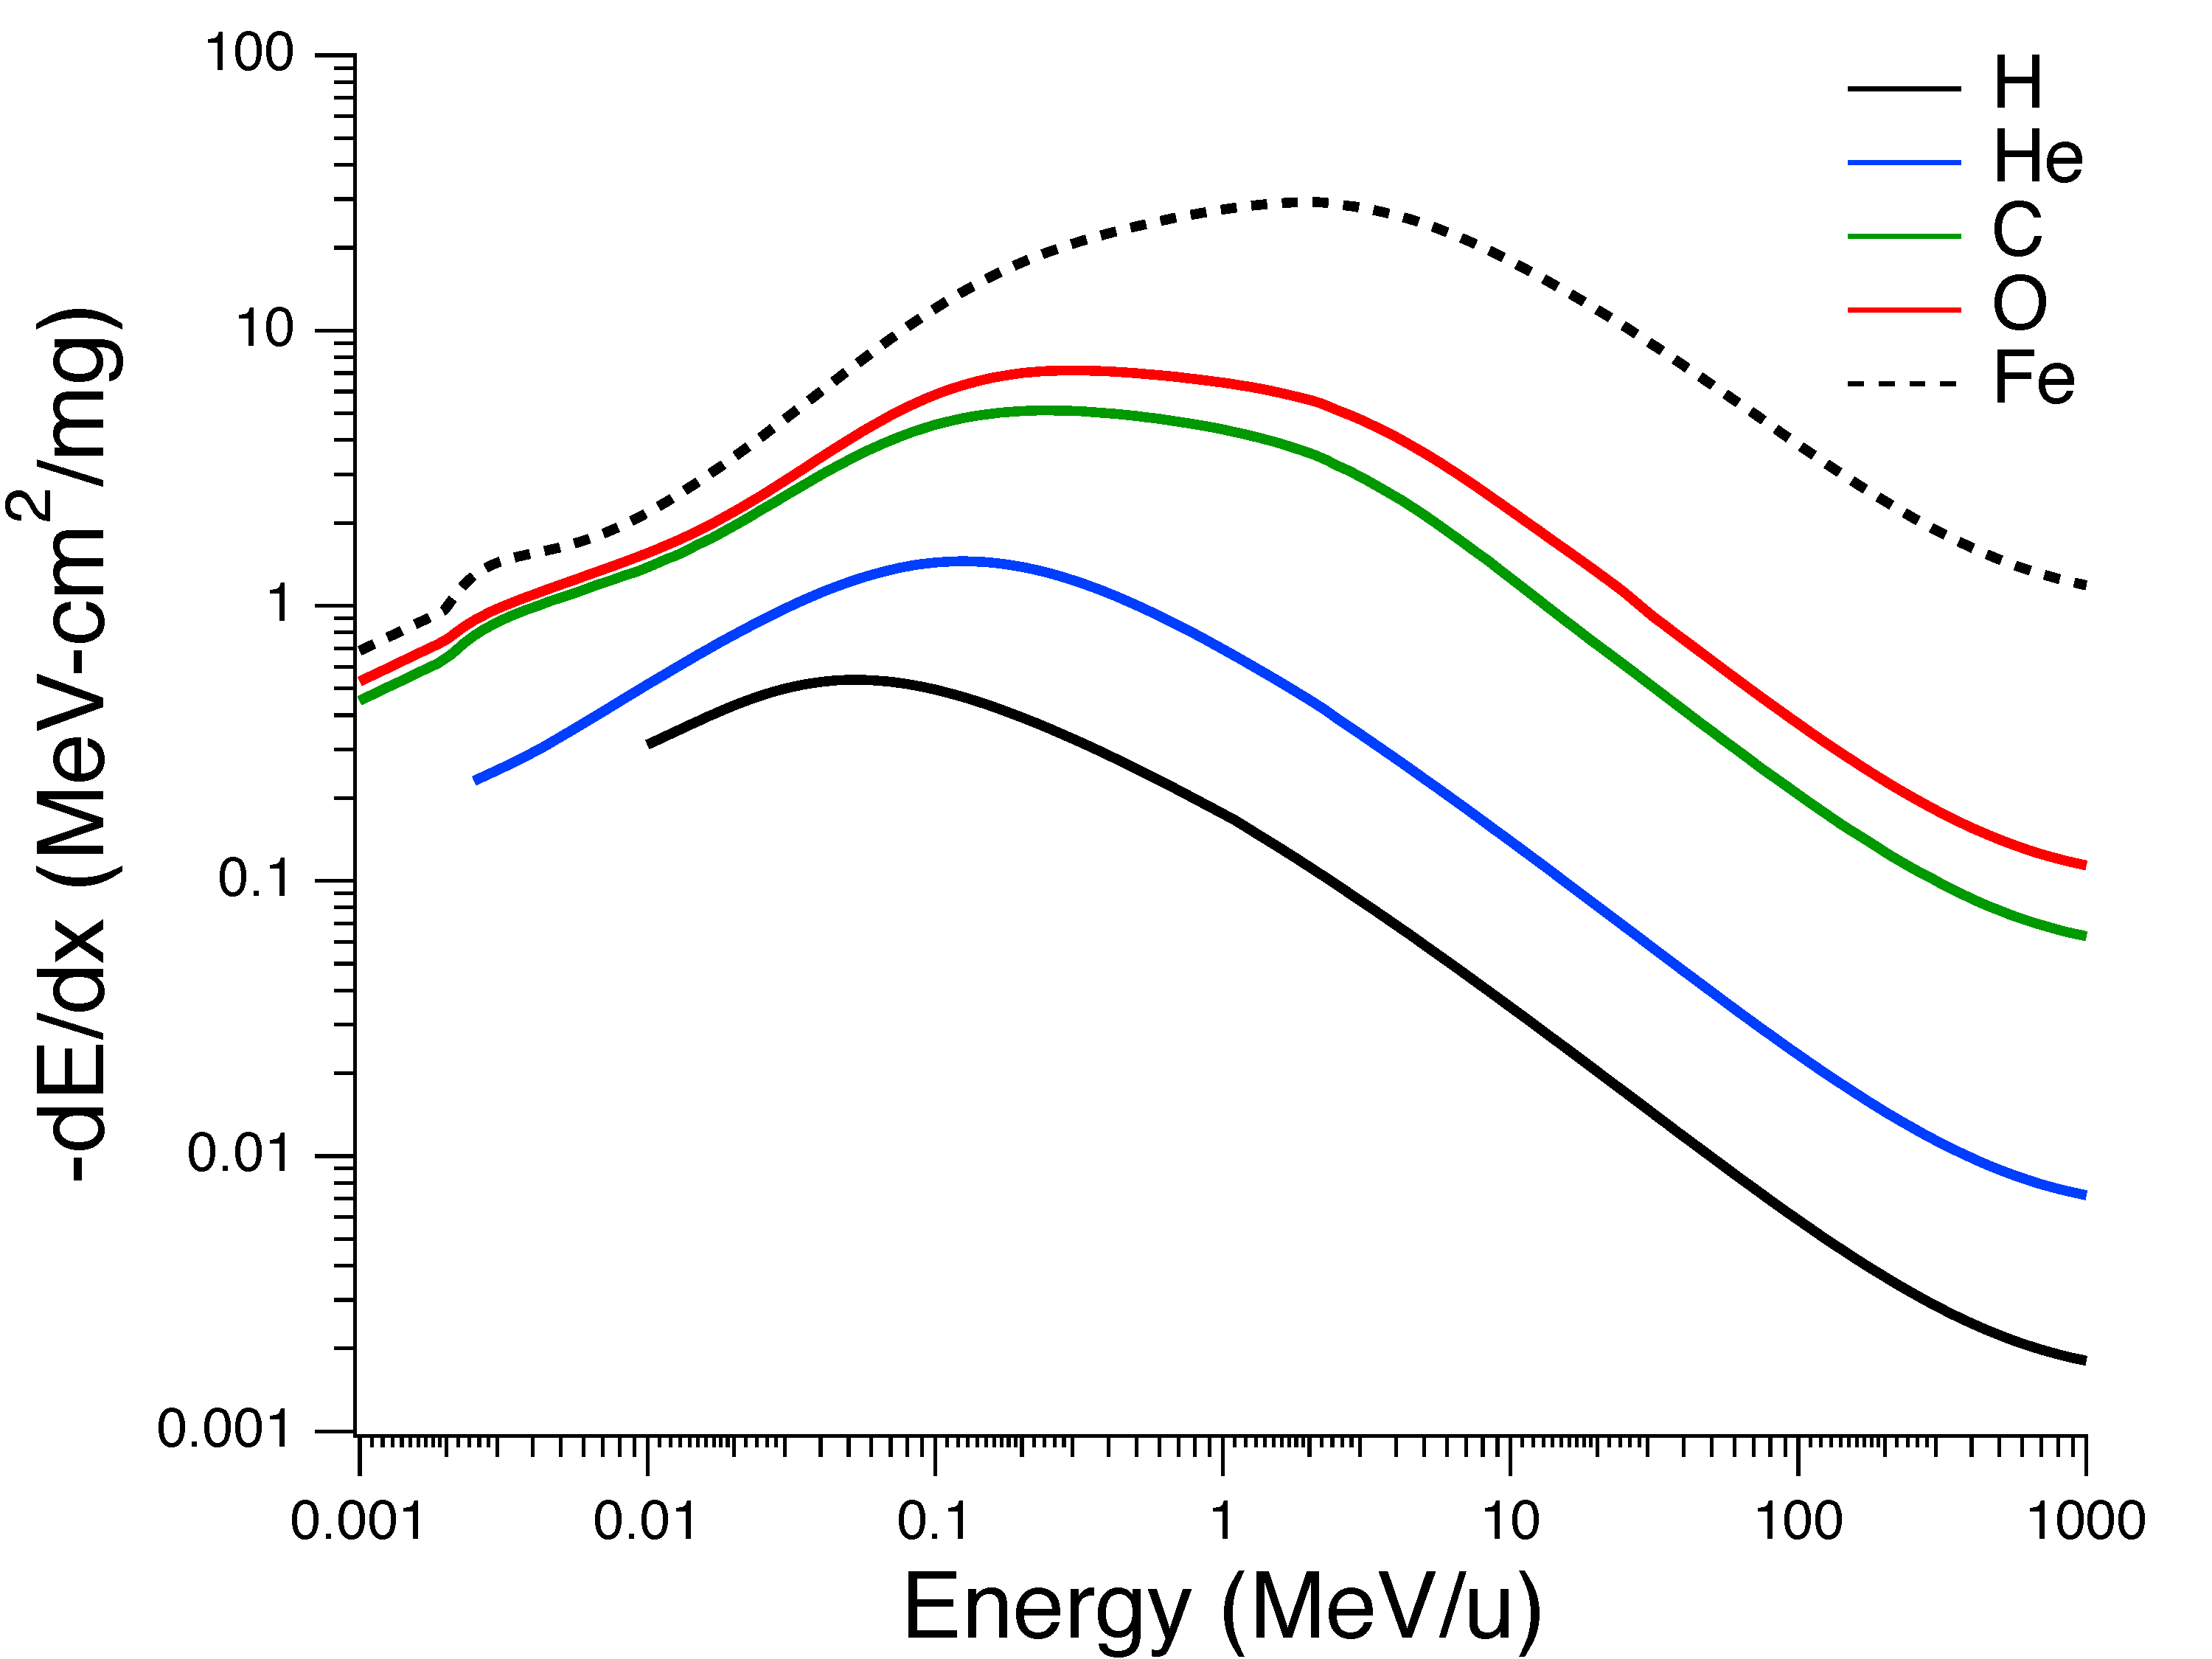
\includegraphics[width=5in]{stopping_vs_energy_mass.pdf}
    \end{center}
    \caption[Stopping power in silicon is plotted as a function of energy per unit mass (MeV/u) for protons, alpha particles, carbon, oxygen, and iron. Stopping power was calculated using the SRIM/TRIM codes.]
    {Stopping power in silicon is plotted as a function of energy per unit mass (MeV/u) for protons, alpha particles, carbon, oxygen, and iron. Stopping power was calculated using the SRIM/TRIM codes \cite{ziegler2010srim}.}
    \label{fig:stopping-power-vs-energy-per-mass}
\end{figure}

The energy lost to the target material through direct ionization generates electron-hole (\emph{e-h}) pairs in semiconductor materials. 
The average energy to create an \emph{e-h} pair in silicon is 3.6~eV \cite{pehl1968accurate,ryan1973precision,scholze2000determination}.
In this sense, one can equate the energy lost by ionizing particles with the generation of charge in semiconductor devices.

The average range of energetic particles in a target material as its trajectory terminates can be accurately described by the continuous slowing down approximation (CSDA). 
The CSDA range assumes that particles transport in a straight line trajectory and variations in energy loss are negligible compared to the total stopping power \cite{bichsel1988straggling}.
It is difficult to define a CSDA range for particles with erratic trajectories due to interactions where large energy loss and large angle deflections occur, this is an especially valid consideration for energetic electrons with energy less than 10~keV.
This CSDA range is obtained by integrating the reciprocal of the total stopping power from the Bethe-Bloch equation, Eq.~\ref{eq:let}, with respect to the incident ion energy.
\begin{equation}
    \label{eq:csda-range}
    R(E) = \int_{E_{abs}}^E \frac{dE'}{S(E')}
\end{equation}
Eq.~\ref{eq:csda-range} describes the CSDA range calculation, where $R(E)$ is the range of a particle with energy $E$ and $E_{abs}$ is the energy at which the particle is assumed to be absorbed (i.e. at rest) within the target material.
It should be noted that Eq.~\ref{eq:csda-range} is only valid for the energy range and conditions where the modified Bethe--Bloch equation is also valid.

The resulting CSDA range approximations in silicon as a function of incident ion energy per unit mass for protons, alpha particles, carbon, oxygen, and iron ions are shown in Fig~\ref{fig:range-vs-energy-per-mass}.
The CSDA range curves shown in Fig.~\ref{fig:stopping-power-vs-energy-per-mass} were calculated using the SRIM/TRIM radiation transport codes \cite{ziegler2010srim}.
\begin{figure}[tb]
    \begin{center}
        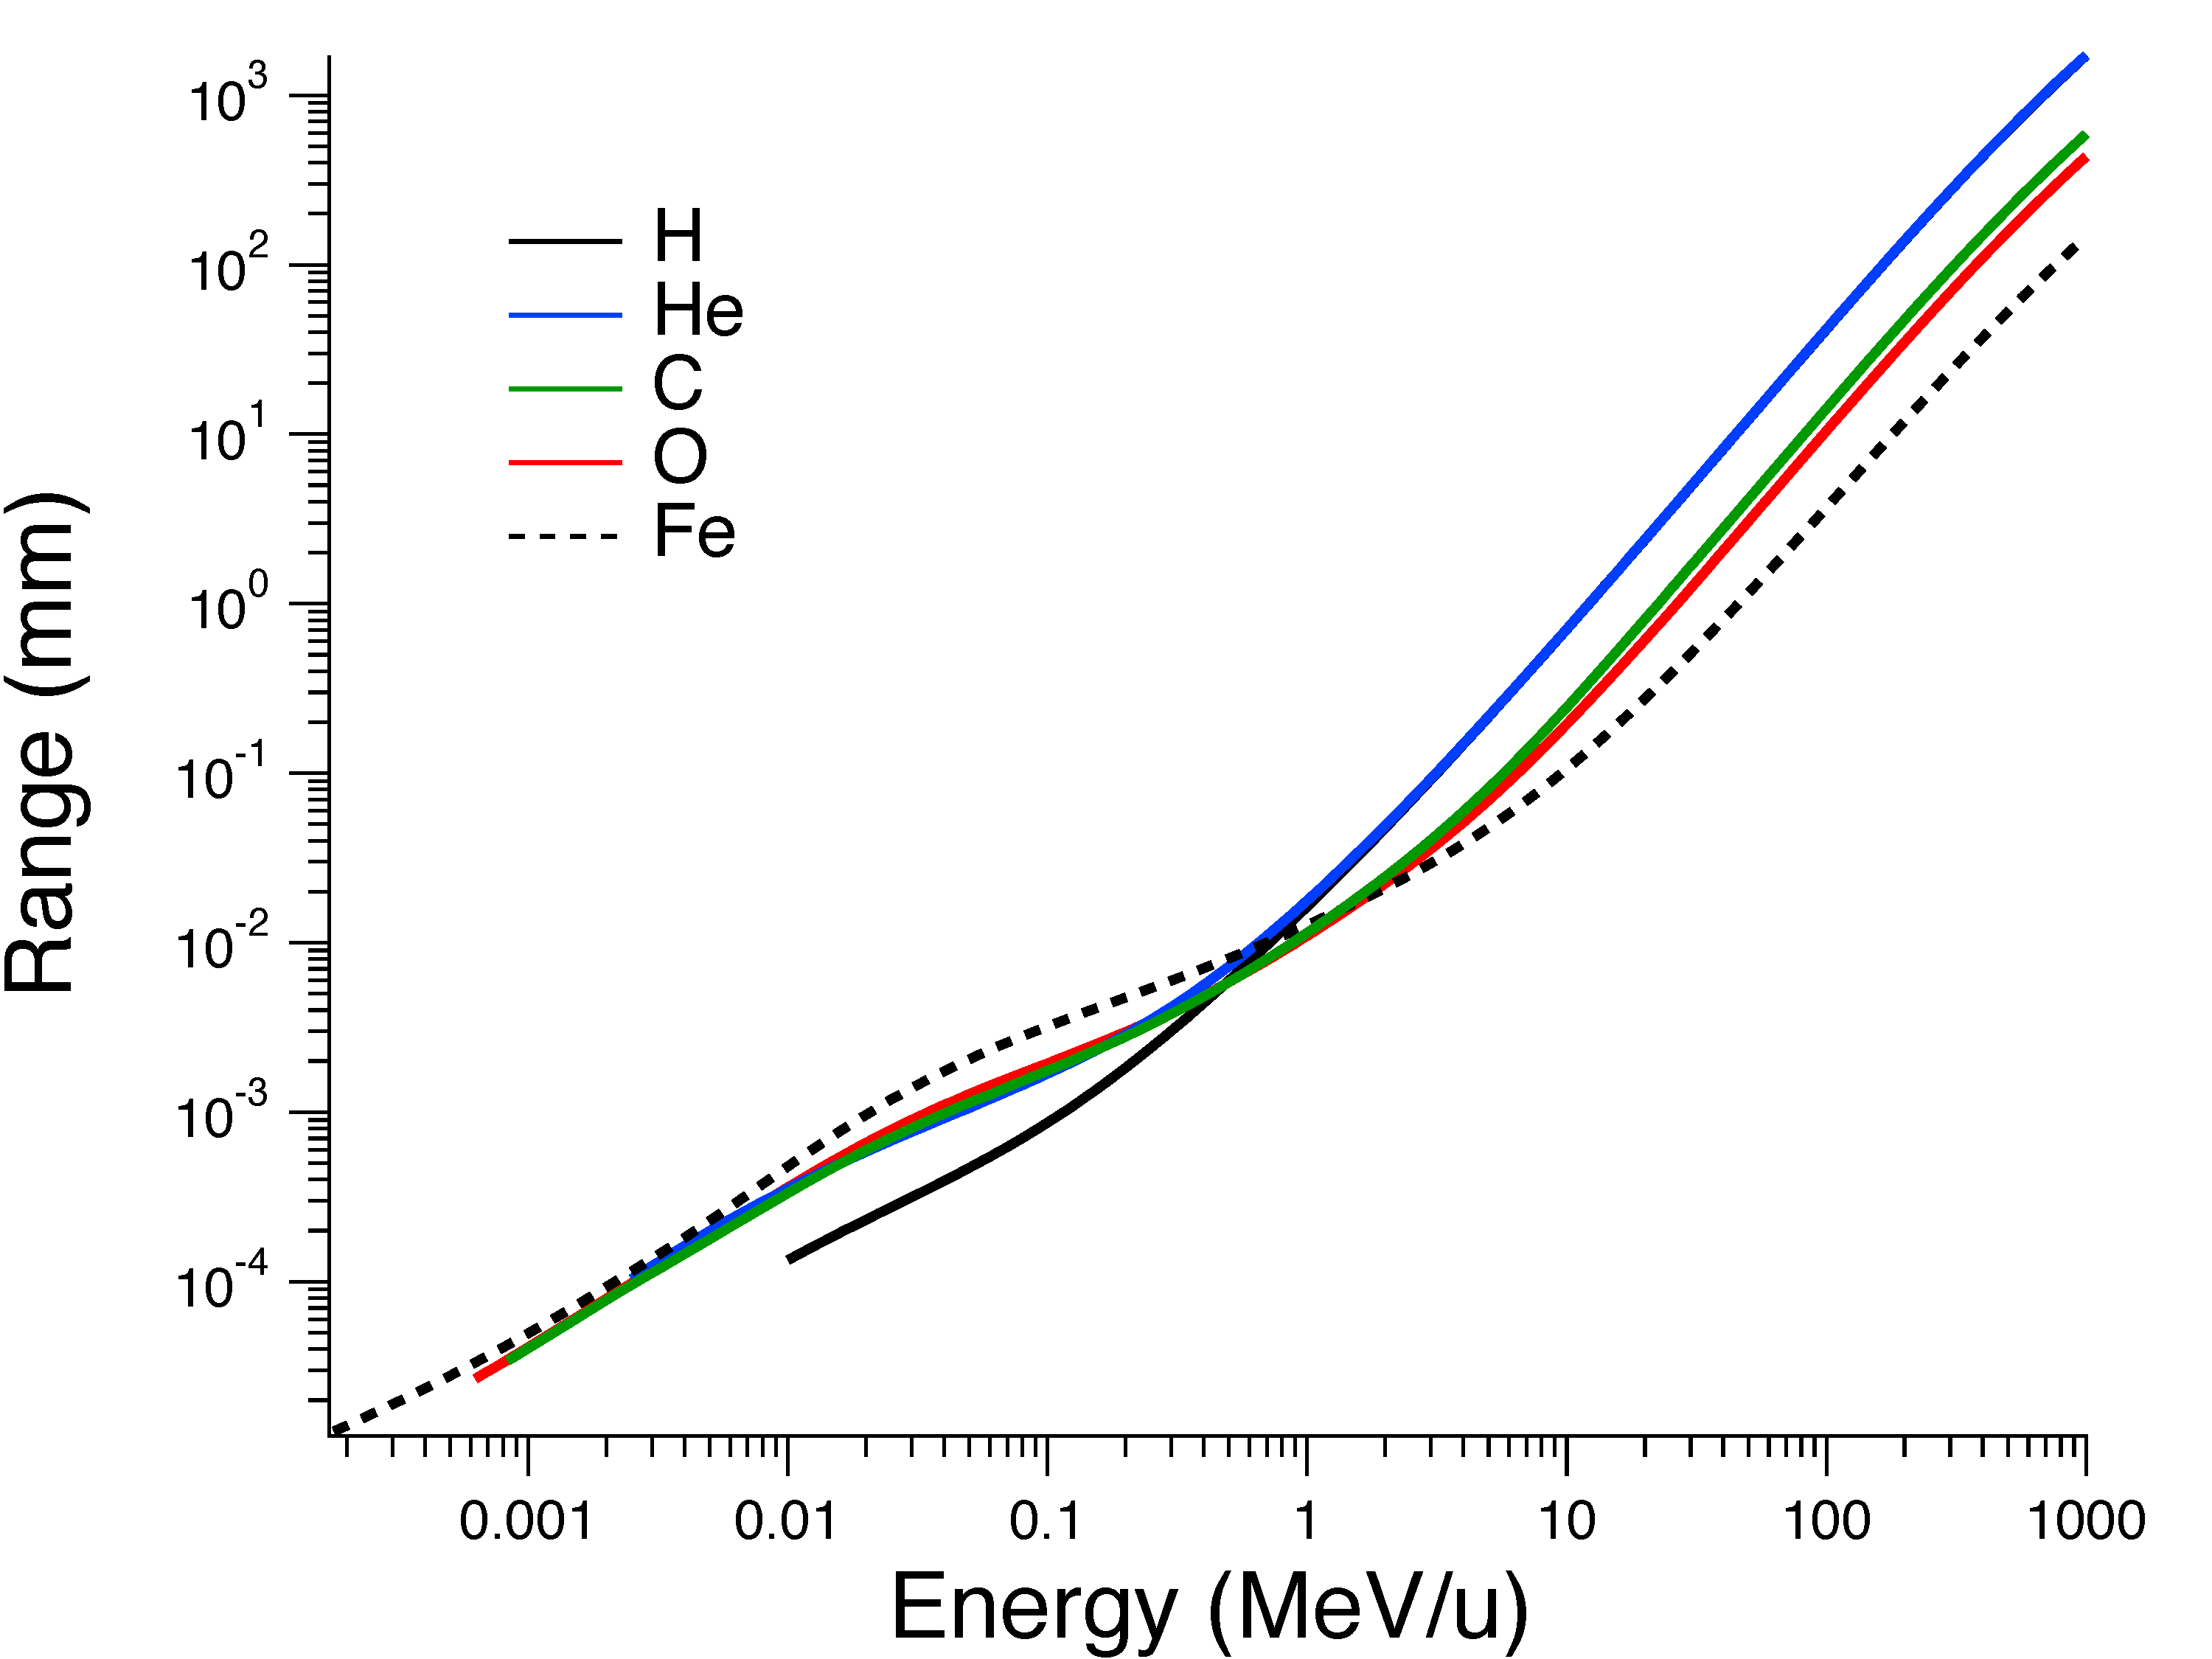
\includegraphics[width=5in]{range_vs_energy-mass.pdf}
    \end{center}
    \caption{CSDA range in silicon as a function of incident ion energy per unit mass for protons, alphas, carbon, oxygen, and iron ions.}
    \label{fig:range-vs-energy-per-mass}
\end{figure}

The range of many of these ion species at energies corresponding to the radiation belts around Earth and Jupiter, GCR, and solar wind environments is much greater than that of the spacing, pitch, and thicknesses of modern semiconductor device structures.
This indicates that single ionizing particle radiation events that occur at large angle of incidence can interact with and perturb multiple devices and circuits.

In 1988, Stapor \emph{et al.} illustrated the potential for differences in the response of microelectronics for two incident ions with similar LET due to differences in the resulting energy deposition profiles \cite{Stapor:1988ws}. 
These conclusions were supported by analyzing the transient response of devices to ions having the same LET but different energies in \cite{HowardJr:2002vg}.
Similar conclusions were reached by Weller and Kobayashi in works published in 2003 and 2004, respectively, which illustrated the importance of energy deposition profiles for proton and alphas in determining the device response to ionizing radiation \cite{Weller:2003je, Kobayashi:2004dg}.

The LET metric has been robust and effective for understanding and modeling the SEU response of SRAMs for many years and continues to serve as the basis for the majority of SEE analysis \cite{Dodd:1998tn,Dodd:1998ua,Dodd:2001tx}.
The application of LET to SEU/SEE analysis relies on the assumption that knowledge about the average energy deposition event is sufficient to predict the circuit response to an ionizing particle event. 
In recent years however, additional physical mechanisms have been required to explain SEU cross sections where LET alone has been insufficient \cite{Reed:2002wn,Kobayashi:2005jt,Reed:2006cx,Reed:2007vz,Warren:2007ca}. 
With the observation of low-energy proton- and muon-induced SEUs the trend towards increased device SEU sensitivity to ionizing radiation and does not appear to be slowing.
The sensitivity of SRAMs to lightly ionizing particles and the concept of critical charge will be discussed in Section~\ref{sec:radiation_effects_on_sram}.
% subsection ion_transport (end)

\subsection{Electron Transport} % (fold)
\label{sub:electron_transport}
Electrons are negatively charged elementary subatomic particles with a mass of 0.511 MeV/c$^2$.
By comparison, the proton mass is 938.23~MeV/c$^2$ and the muon mass is 105.7~MeV/c$^2$, making the electron 1836 and 206 times lighter than other common singly-charged particles.
Energetic electrons interact with a target material predominantly through electromagnetic processes. 
Two energy loss mechanisms are important for electrons interacting with a target medium, inelastic scattering with atomic electrons and elastic scattering with target nuclei.
\begin{figure}[tb]
    \begin{center}
        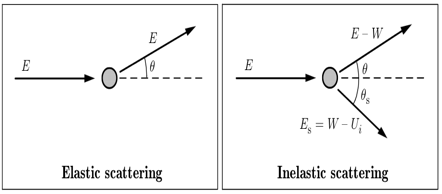
\includegraphics[width=5in]{delta-ray-scattering-salvat.png}
    \end{center}
    \caption[Elastic and inelastic scattering of an incident electron with initial energy $E$.]{Elastic and inelastic scattering of an incident electron with initial energy $E$ \cite{Salvat:ue}.}
    \label{fig:electron-scattering-elastic-inelastic}
\end{figure}

Inelastic collisions are the dominant energy loss mechanism for low and intermediate electron energies, where the incident electron interacts with atomic electrons of the target material.
These are interactions that produce \emph{e-h} pairs, ionization, or result in the ejection of additional energetic electrons from the band structure of the material.
The initial formalism of inelastic scattering with single atoms or molecules was made by Bethe in \cite{bethe1930theorie,bethe1932bremsformel} by considering a plane-wave using the Born approximation.
This theory was later extended by Fano for inelastic scattering of electrons in condensed matter \cite{fano1964penetration}.
The impact on the incident electron can be accurately described by the energy loss, $W$, and the polar and azimuthal scattering angles, $\phi$ and $\theta$.

A cartoon of an inelastic scattering event can be seen on the right hand side of Fig.~\ref{fig:electron-scattering-elastic-inelastic}. 
The energy transferred to the atomic system, $W$, is equivalent to the energy lost by the incident electron.
Most interactions with atomic electrons result in the generation of \emph{e-h} pairs in semiconductors.
However, if the energy loss by the incident electron is in excess of the shell binding energy the interaction results in the emission of an energetic electron that is free of the material band structure, also called a $\delta$-ray, with energy equal to $E_s$, where this is the difference between the total energy lost by the incident electron, $W$, and the $i$th shell binding energy, $U_i$.
The relaxation of the excited atomic state, the vacancy of the $i$th shell state, involves the emission of fluorescent radiation in the form of Auger electrons or soft X-rays with energy equal to the $i$th shell binding energy.
The relatively equal masses involved in inelastic scattering, which are essentially electron--electron interactions, result in angular deflections of the incident electron.
Angular deflections of energetic electrons transporting through material are important parameters that make determining the range of low energy electrons, lower than a few tens of keV, particularly difficult.

The second important interaction mechanism for electrons in this work is the elastic scattering of incident electrons with isolated atomic nuclei.
Here the elastic scattering event is defined to be an interaction between an energetic electron and a target nuclei where the initial and final quantum states of the target atom are the same, usually the ground state.
The elastic scattering with target nuclei result in large angle deflections of incident energetic electrons.
A cartoon of an elastic scattering event is shown on the left hand side of Fig.~\ref{fig:electron-scattering-elastic-inelastic}.
For elastic scattering events, there is a small transfer of energy from the incident electron to the target nuclei, potentially resulting in the emission of a recoil atom.
Because of the large mass of the target nuclei relative to the electron mass, the average energy lost by an incident electron in elastic scattering events is a \emph{small} fraction of its initial energy.
For electrons with energy of 30~keV, the energy lost in elastic scattering events is on the order of a few meV \cite{Salvat:ue}.
Scattering events, of the elastic and inelastic variety, both contribute to large angle deflections of energetic electrons.
These large angle deflections make approximating the range of electrons in matter through methods like the CSDA range particularly difficult at low energies (less than 10~keV).

Because of their small mass, electrons undergo Bremsstrahlung and Cerenkov radiative processes.
The total stopping power of electrons is represented as the superposition of the collision and radiative stopping power processes.
\begin{equation}
    \label{eq:elec-let-superpos}
    -\left(\frac{dE}{dx}\right)_{total} = S_{coll}(E) + S_{rad}(E)
\end{equation}
In Eq.~\ref{eq:elec-let-superpos}, $S_{coll}(E)$ and $S_{rad}(E)$ are the stopping power contributions from collisions and radiative processes respectively.
These additional energy loss processes do not occur for heavier particles (at least until \emph{extremely} high energies) and are important for understanding electron transport, but have few consequences for this work since they are prevalent at energies in excess of 10~MeV.
Consequently, this dissertation only considers the contribution of inelastic and elastic scattering interactions between the incident electron and the target material.
With appropriate modifications to the Bethe-Bloch formula of Eq.~\ref{eq:bethe-bloch-corr-ion} it can be shown that the maximum single electron--electron scattering event energy loss is one half of the initial electron energy, $E_i/2$ \cite{segre1964nuclei,1982spre.reptR....B,Salvat:ue}.
Electrons are therefore capable of depositing large amounts of energy within small spatial regions.

\begin{figure}[tb]
    \begin{center}
        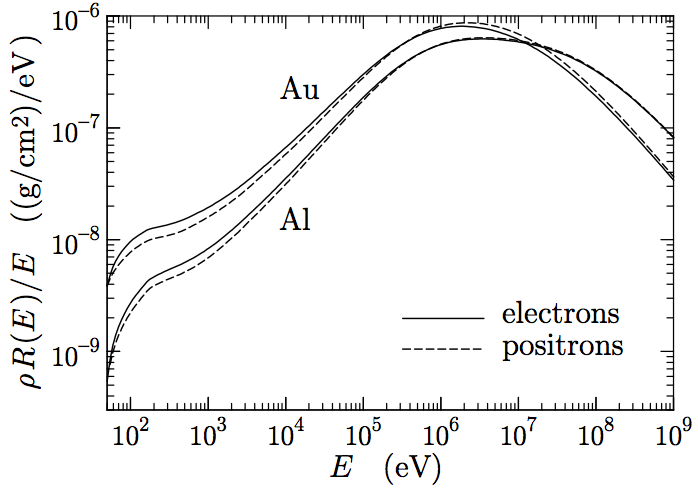
\includegraphics[width=5in]{electrons-csda-range.png}
    \end{center}
    \caption[CSDA ranges for electrons and positrons in aluminum and gold as functions of kinetic energy of the particle.]{CSDA ranges for electrons and positrons in aluminum and gold as functions of kinetic energy of the particle \cite{Salvat:ue}.}
    \label{fig:csda-range-electrons}
\end{figure}

The range of energetic electrons in a target material can be approximated using Eq.~\ref{eq:csda-range}.
The approximate CSDA range of electrons (and positrons) is shown in Fig.~\ref{fig:csda-range-electrons}.
Below energies of approximately 1~MeV, electrons follow a similar trend as the heavy ions shown in Fig.~\ref{fig:range-vs-energy-per-mass}, where the incident particle range increases with increasing energy.
Electrons and positrons exhibit a decrease in range with increasing energy above energies of 10~MeV due to the radiative energy loss processes (Bremsstrahlung and Cerenkov).
% subsection electron_transport (end)

\subsection{Photon Transport} % (fold)
\label{sub:photon_transport}
Photons are elementary particles that exhibit the properties of waves and particles (known as Wave--Particle duality) and interact through the electromagnetic force.
Three physical processes dominate energy loss by incident photons in matter, the photoelectric effect, Compton scattering, and pair production. 
While pair production is an important interaction mechanism, this discussion focuses on the photoelectric and Compton scattering effects, which are most relevant to the work presented in Chapters~\ref{cha:experimental_investigation_of_electron_induced_seus} and \ref{ch:simulation_of_electron_induced_seus}.
Fig.~\ref{fig:gamma_energy_vs_mat_z} shows the energy dependence of the three dominant physical processes for photons incident in material.
\begin{figure}[tb]
    \centering
        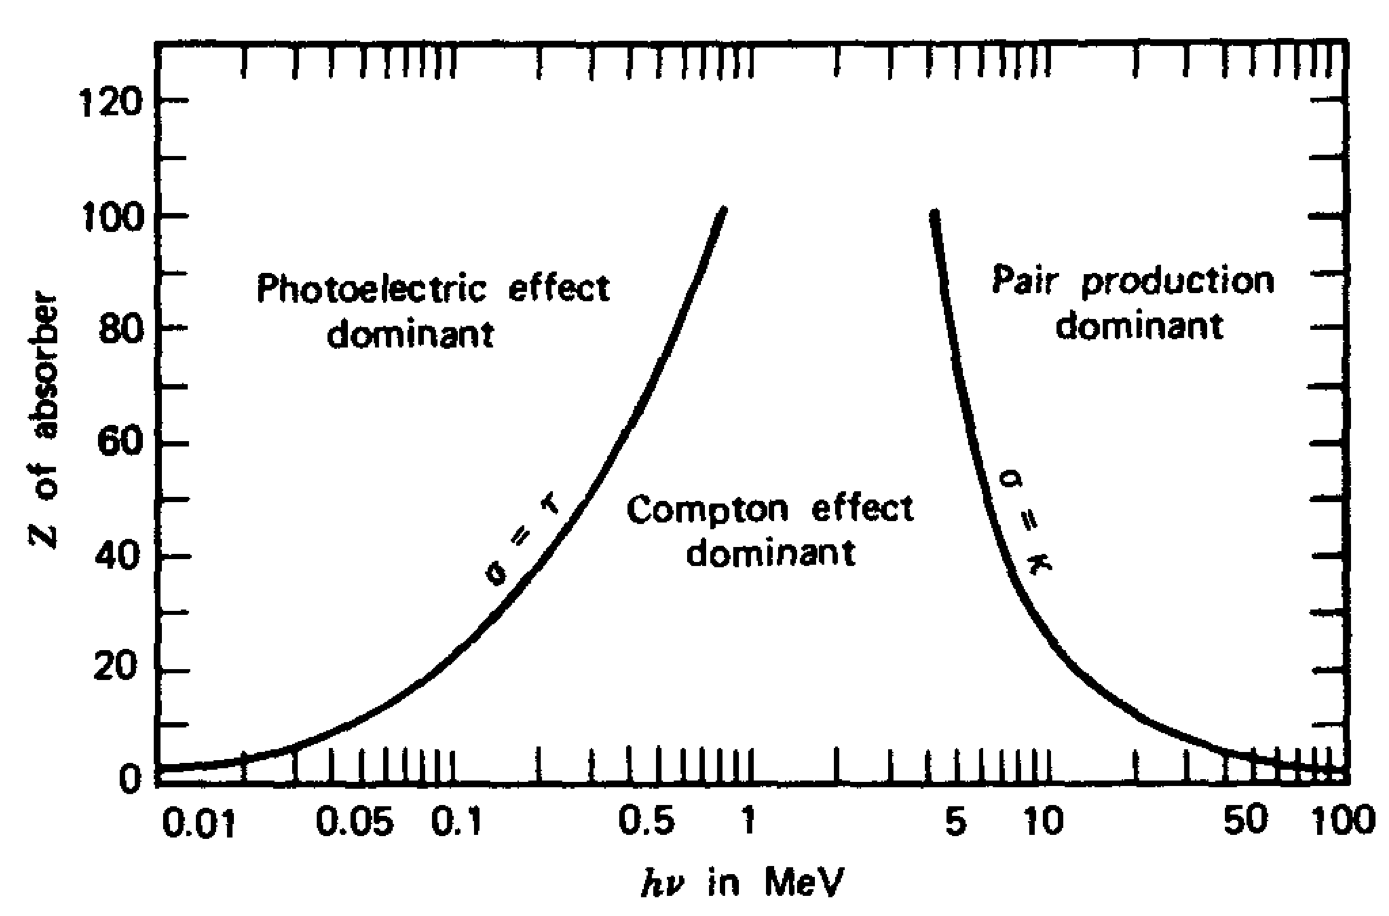
\includegraphics[width=5in]
        {gamma_energy_vs_matz.png}
    \caption[The energy dependence of the three major types of photon interactions are shown. The lines shows the values of material $Z$ and photon energy $\hbar \omega$ for which the two neighboring effects are approximately equal.]{The energy dependence of the three major types of photon interactions are shown. The lines shows the values of material $Z$ and photon energy $\hbar \omega$ for which the two neighboring effects are approximately equal \cite{Knoll:2010vq}.}
    \label{fig:gamma_energy_vs_mat_z}
\end{figure}

In silicon, the dominant interaction of photons with energy less than 70~keV is the photoelectric effect. 
The photoelectric effect is a point interaction where the incident photon is completely absorbed by a target atom, leaving the atom in an excited state.
Fig.~\ref{fig:photoabsorption} shows a cartoon description of a photoabsorption event from \cite{alpen1997radiation}.
An energetic photo-electron is ejected from the material band structure as a result of the excited atomic state.
Subsequently an X-ray is emitted with energy equal to the binding energy, $E_b$, of the generated photo-electron due to the relaxation of an electron from an \emph{L} or \emph{M}--shell into the lower energy state.
Generated photo-electrons are typically emitted omnidirectionally from a tightly bound state, such as the \emph{K}--shell, assuming the incident photon has energy greater than the binding energy of the \emph{K}--shell.
The energy transferred to the photo-electron can be described as
\begin{equation}
    \label{eq:photo_electron_energy}
    E_{e^-} = \hbar \omega - E_{b}
\end{equation}
where $\hbar \omega$ is the energy of the photon and $E_b$ is the binding energy of the photo-electron in its initial shell.
For highly energetic photons (where $\hbar 
\omega \gg E_b$) most of the absorbed photon energy is transferred to the photo-electron.

\begin{figure}[tb]
    \begin{center}
        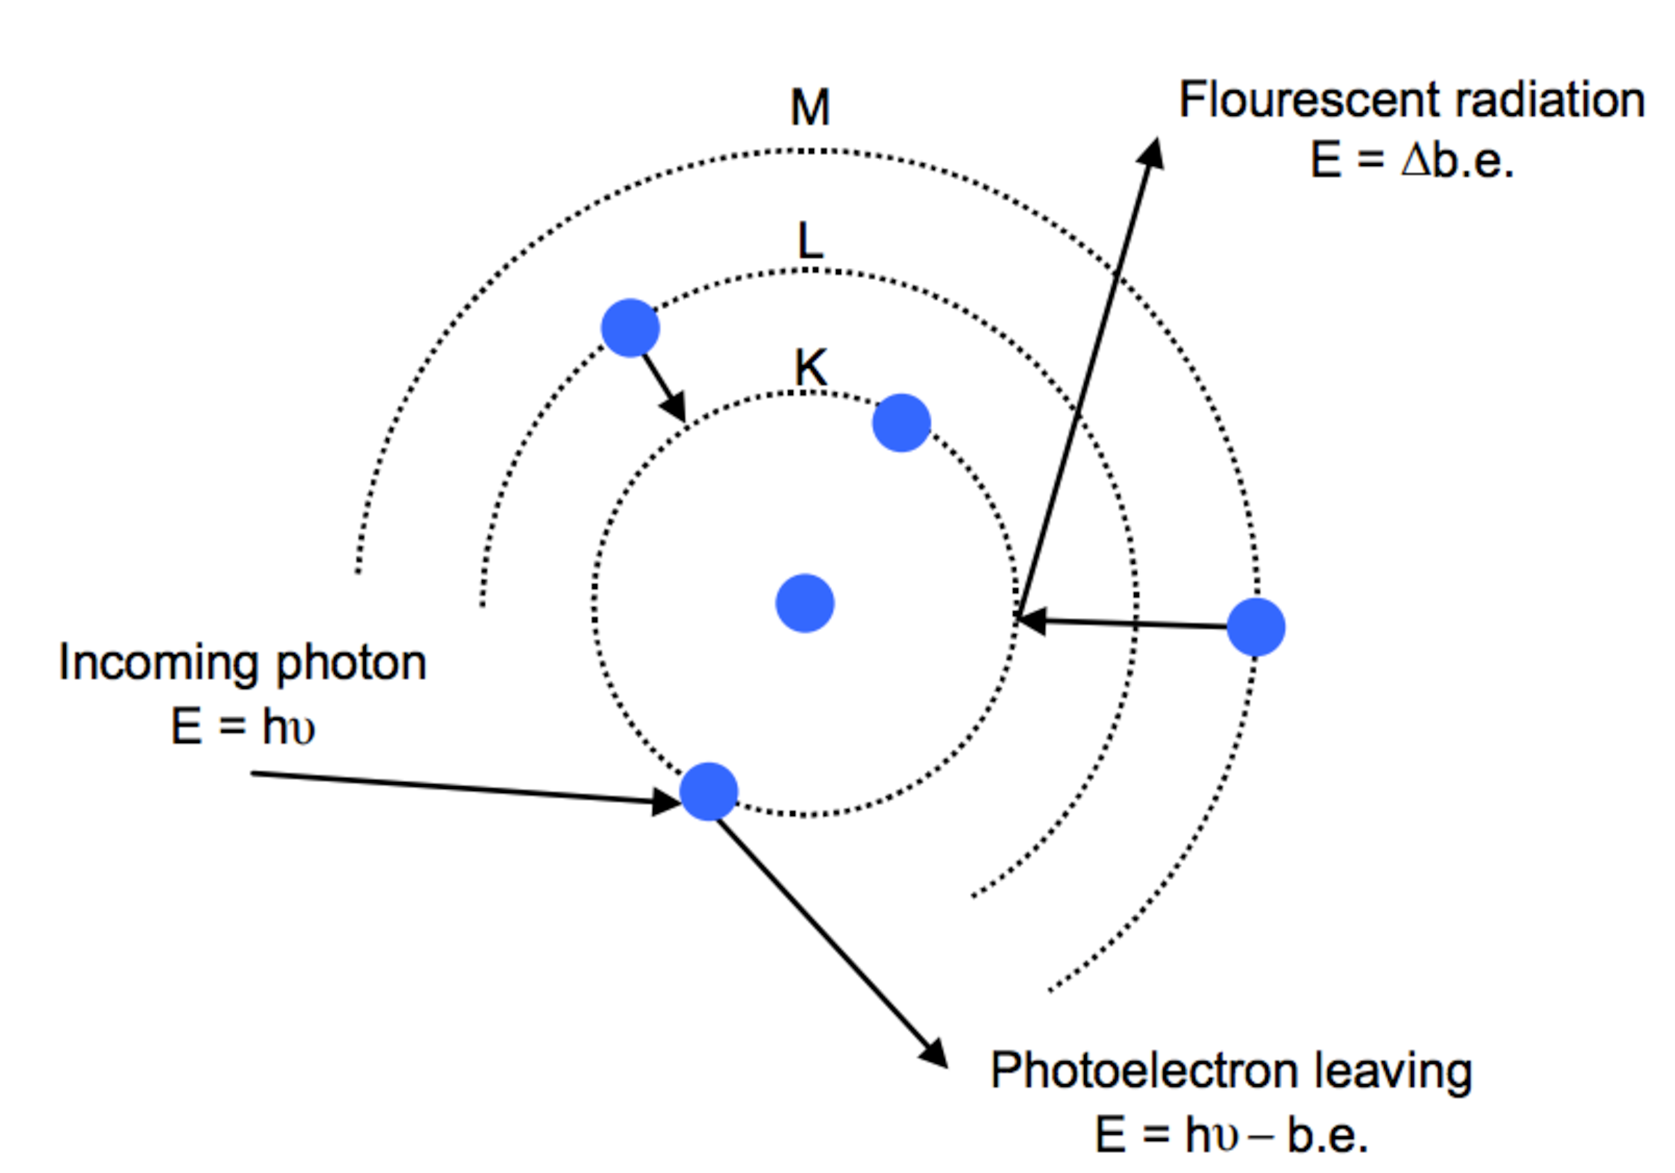
\includegraphics[width=4.5in]{photoabsorption.pdf}
    \end{center}
    \caption[Absorption of an incident photon with energy $\hbar \omega$ resulting in the generation of an energetic photo-electron and emission of fluorescent radiation.]{Absorption of an incident photon with energy $\hbar \omega$ resulting in the generation of an energetic photo-electron and emission of fluorescent radiation \cite{alpen1997radiation}.}
    \label{fig:photoabsorption}
\end{figure}
\begin{figure}[tb]
    \centering
        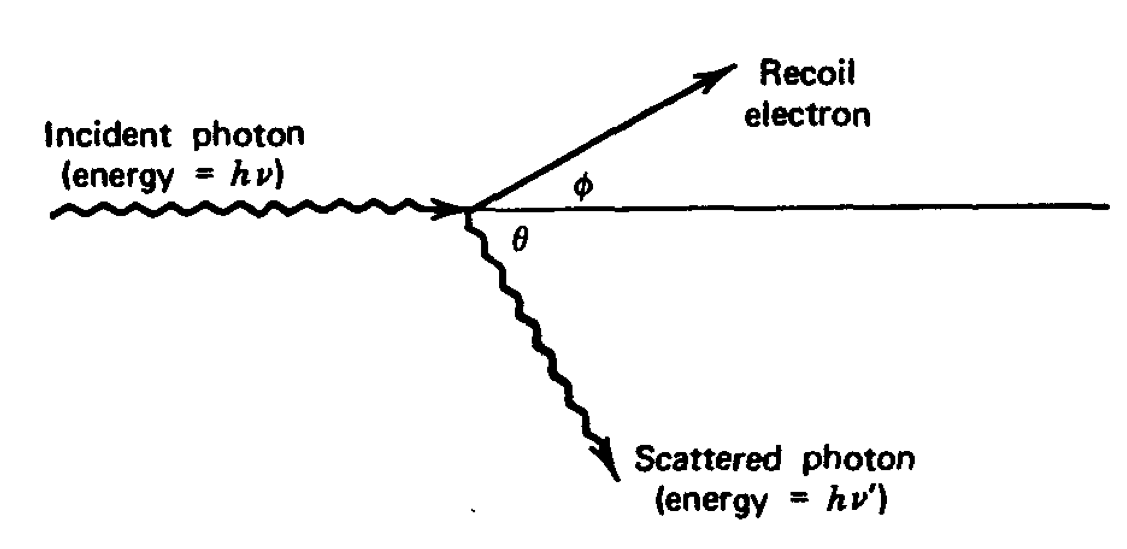
\includegraphics[width=5in]
        {compton_scattering_diagram2.png}
    \caption[Diagram of a Compton scattering event between an incident photon with energy $\hbar \omega$ and an electron.]{Diagram of a Compton scattering event between an incident photon with energy $\hbar \omega$ and an electron.}
    \label{fig:compton_scattering_diagram2}
\end{figure}

Photons with energy in the range of 70~keV to 12~MeV interact primarily through the Compton scattering process in silicon.
The Compton effect involves the incoherent scattering of a photon by a bound electron.
The scattering event results in energy loss by the incident photon, corresponding to a reduction in frequency, and the generation of a \emph{recoil} electron.
A diagram of a Compton scattering event is shown in Fig.~\ref{fig:compton_scattering_diagram2}.
Since the collision must obey both conservation of energy and momentum it can be shown that the transfer of energy from the photon can be described by
\begin{equation}
    \label{eq:compton_energy_transfer}
    E_{e} = \hbar \omega \frac{\frac{\hbar \omega}{m_{e} c^2}(1-\cos\theta)}{1 + \frac{\hbar \omega}{m_e c^2}(1-\cos\theta)}
\end{equation}
where $\hbar \omega$ is the energy of the incident photon, $m_{e}c^2$ is the electron rest energy, and $\theta$ is the scattering angle of the photon as seen in Fig.~\ref{fig:compton_scattering_diagram2}.

Eq.~\ref{eq:compton_energy_transfer} shows thats for small scattering angles (where $\theta \approx 0$) very little energy is transferred to the generated recoil electron.
The maximum energy transfer occurs when the incident photon is back-scattered (where $\theta \approx \pi$) and the recoil electron has initial momentum along the incident photons original trajectory.
The initial energy of all recoil electrons generated in Compton scattering events fall within the Compton continuum, an energy range bounded by the minimum and maximum energy transferred in a scattering event.

The total attenuation cross-section, $\mu$, can be expressed as the superposition of the attenuation cross-section for each physical process shown in Fig.~\ref{fig:gamma_energy_vs_mat_z}.
The expression for total attenuation cross-section can be expressed as 
\begin{equation}
    \label{eq:total_photon_cs}
    \mu = \tau + \sigma + \kappa
\end{equation}
where $\tau$, $\sigma$, and $\kappa$ are the photoelectric, Compton, and pair production cross-sections, respectively.
The total attenuation cross section, $\mu$, (in units of cm$^2$/g) versus incident photon energy in silicon is shown in Fig.~\ref{fig:atten_cs_in_si}.
The discontinuity seen at 1.839~keV corresponds to the silicon \emph{K}-shell edge, this corresponds to the minimum energy required to emit an electron from the \emph{K}-shell \cite{Henke:1993tq}.
For incident photons with energy less than 1.839~keV, interactions involve the emission of photo-electrons from the \emph{L}- or \emph{M}-shells.
The absorption edge corresponding to the $L_1$, $L_2$, and $L_3$-shells in silicon occur at 149.7~eV, 99.8~eV, and 99.2~eV, respectively.

\begin{figure}[tb]
    \begin{center}
        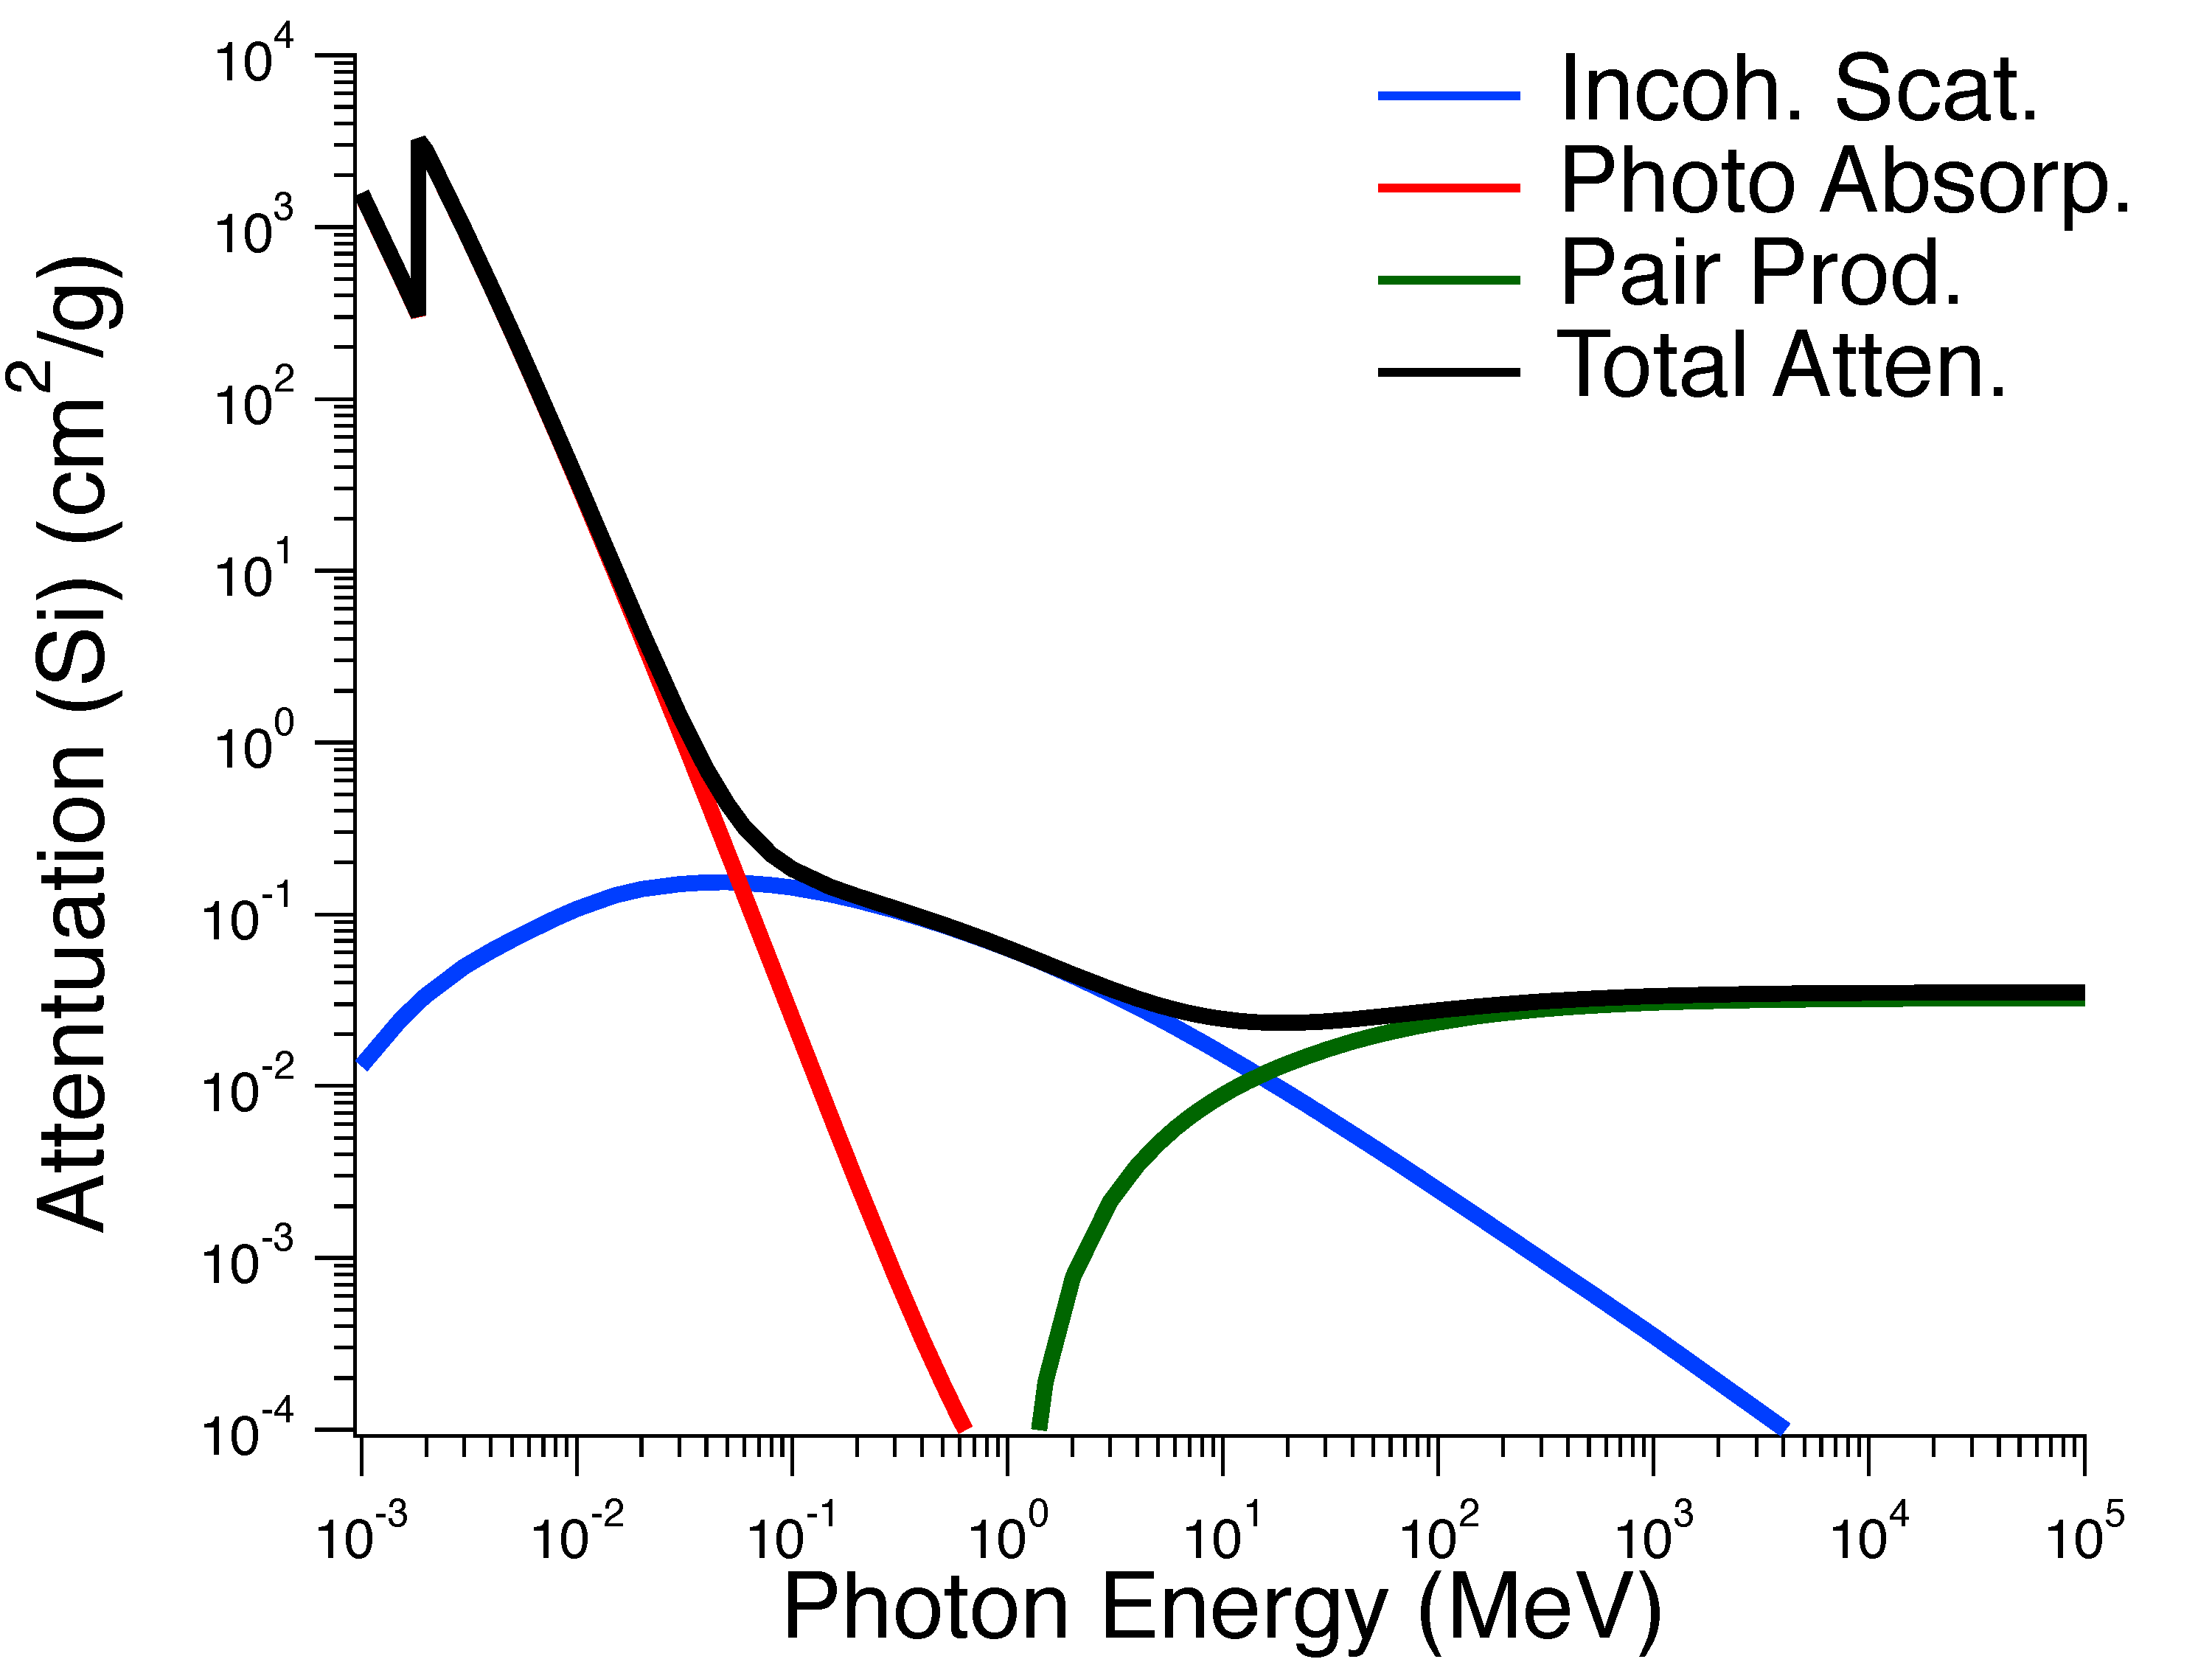
\includegraphics[width=5in]{photon_scat_cross_section.pdf}
    \end{center}
    \caption{The attenuation cross-section, $\mu$, versus incident photon energy in silicon.}
    \label{fig:atten_cs_in_si}
\end{figure}

The attenuation of energetic photons transporting through material can be calculated using the Beer--Lambert law \cite{ingle1988spectrochemical}, which is given as
\begin{equation}
    \label{eq:beer_lambert}
    N = N_0(E) e^{-(\mu(E)/\rho) (\rho x)}
\end{equation}
where $N_0(E)$ is the initial number of photons with energy $E$, $\mu(E)/\rho$ is the energy-dependent mass attenuation coefficient (obtained from Fig.~\ref{fig:atten_cs_in_si}), and $\rho x$ is the mass thickness of the target material.
Eq.~\ref{eq:beer_lambert} provides a straight forward method for calculating the attenuation of photons and can be used to determine the energy absorbed within a specific range of the target material.
% subsection photon_transport (end)
% section basic_interaction_mechanisms (end)

\section{Basic SRAM Topology and Operation} % (fold)
\label{sec:basic_sram_topology_and_operation}
As CMOS feature sizes have decreased, a corresponding reduction in areal density of individual memory cells has resulted in lowering of the cost per bit.
This has enabled access to low-cost, high-speed memory for many applications.
These attributes have made SRAMs ideal for use in microprocessor cache memory, general use registers, FPGAs, and other applications.

While SRAM implementations can be expensive, in terms of area, they are typically more desirable than conventional dynamic random access memory (DRAM) in terms of speed and power consumption.
Since an SRAM cell takes up more area than DRAM cells in the same technology node, these benefits come at the expense of increased area and cost.
Basic SRAM implementations offer significant advantages over DRAM in terms of power consumption because they do not require the refreshing of data while powered, putting SRAM in a class known as volatile memories.
SRAMs are ideal where bandwidth, power, or both are a primary design consideration.

\begin{figure}[tb]
    \centering
        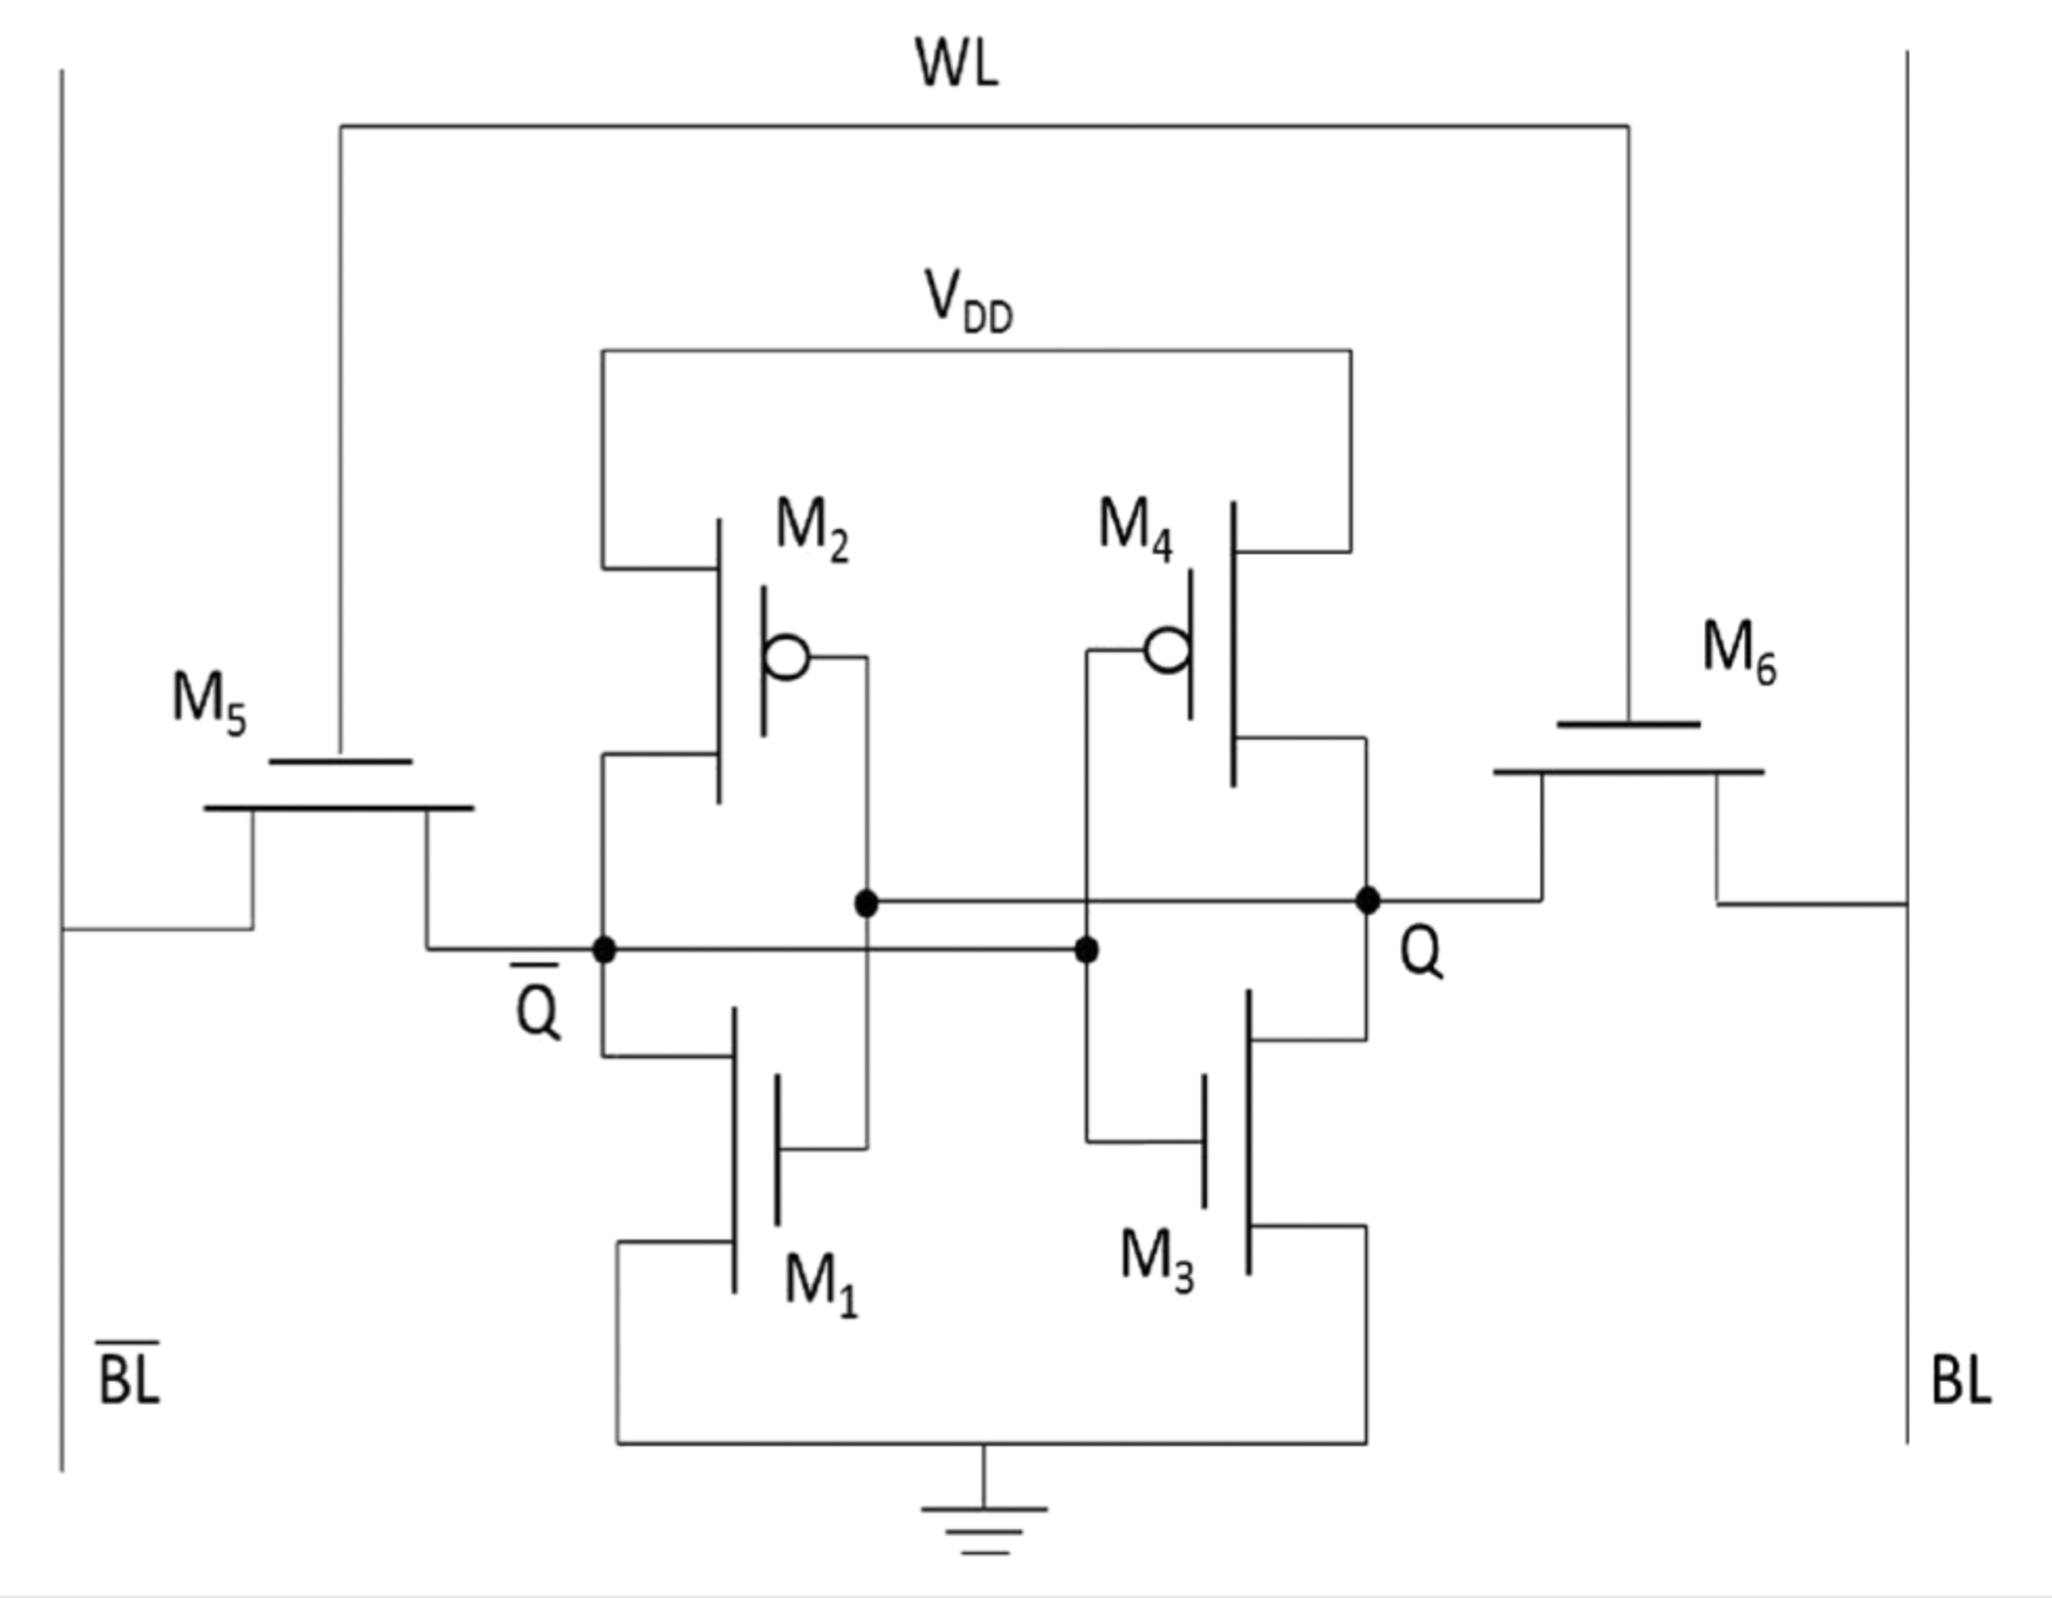
\includegraphics[width=4.5in]
        {SRAM_Cell_(6_Transistors).pdf}
    \caption{Basic SRAM circuit topology consists of two cross coupled inverters and two access transistors.}
    \label{fig:SRAM_Cell}
\end{figure}

The basic topology of a standard six transistor (6T) SRAM can be seen in Fig.~\ref{fig:SRAM_Cell}. 
While other SRAM implementations are possible, including non-volatile topologies, this dissertation only considers the standard 6T-SRAM cell.
The basic SRAM cell stores information on two cross-coupled inverters, consisting of four transistors (M1--M4), that form a basic latch, enabling the stable states of either \emph{0} or \emph{1}.
Two additional access transistors (M5 and M6) allow access operations to the SRAM cell.

An SRAM cell has three standard modes of operation, write, read, and standby.
A write operation occurs by applying a voltage to the bit line and its complement ($BL$ and $\overline{BL}$) and asserting the word line.
The voltage applied to the bit lines should have a large potential difference such that the state is quickly reinforced by the two inverters.
A potential difference close to the supply voltage ($V_{DD}$) is quite common in standard technology implementations.
A read operation occurs when the bit lines are left floating while the word line is asserted.
Using peripheral circuitry (not shown), a high-speed sense amplifier compares the voltage difference between the bit line and its complement, outputs the state of the cell to subsequent buffers, and is then passed to the output bus.
Standby mode occurs when the word line is left floating, during which time the access transistors are ``off'' and the inverters continually reinforce the present state of the SRAM cell.
Standby mode is the ``idle state'' of an SRAM cell and results in the lowest power consumption of all standard SRAM operating modes.

A common practice to reduce power consumption while operating in standby mode is to lower the supply voltage to the SRAM below the nominal supply voltage.
This is a method known as dynamic voltage, frequency scaling at the systems level and is used to reduce power consumption when operating frequency is a secondary priority \cite{semeraro:2002dvfs,david:2011dvfs}.
The trade-off is typically made in applications where low-power is a primary operating parameter such as medical implant devices, mobile communications, and mobile computing.
For these applciations SRAMs are designed to remain stable and completely functional at 70--80\% of the nominal supply voltage while maintaining valid information.
While both bit lines are not required for proper SRAM cell operation, utilizing both the bit line and its complement increases the circuits noise margin and results in increased read and write speed.

\begin{figure}[tb]
    \begin{center}
        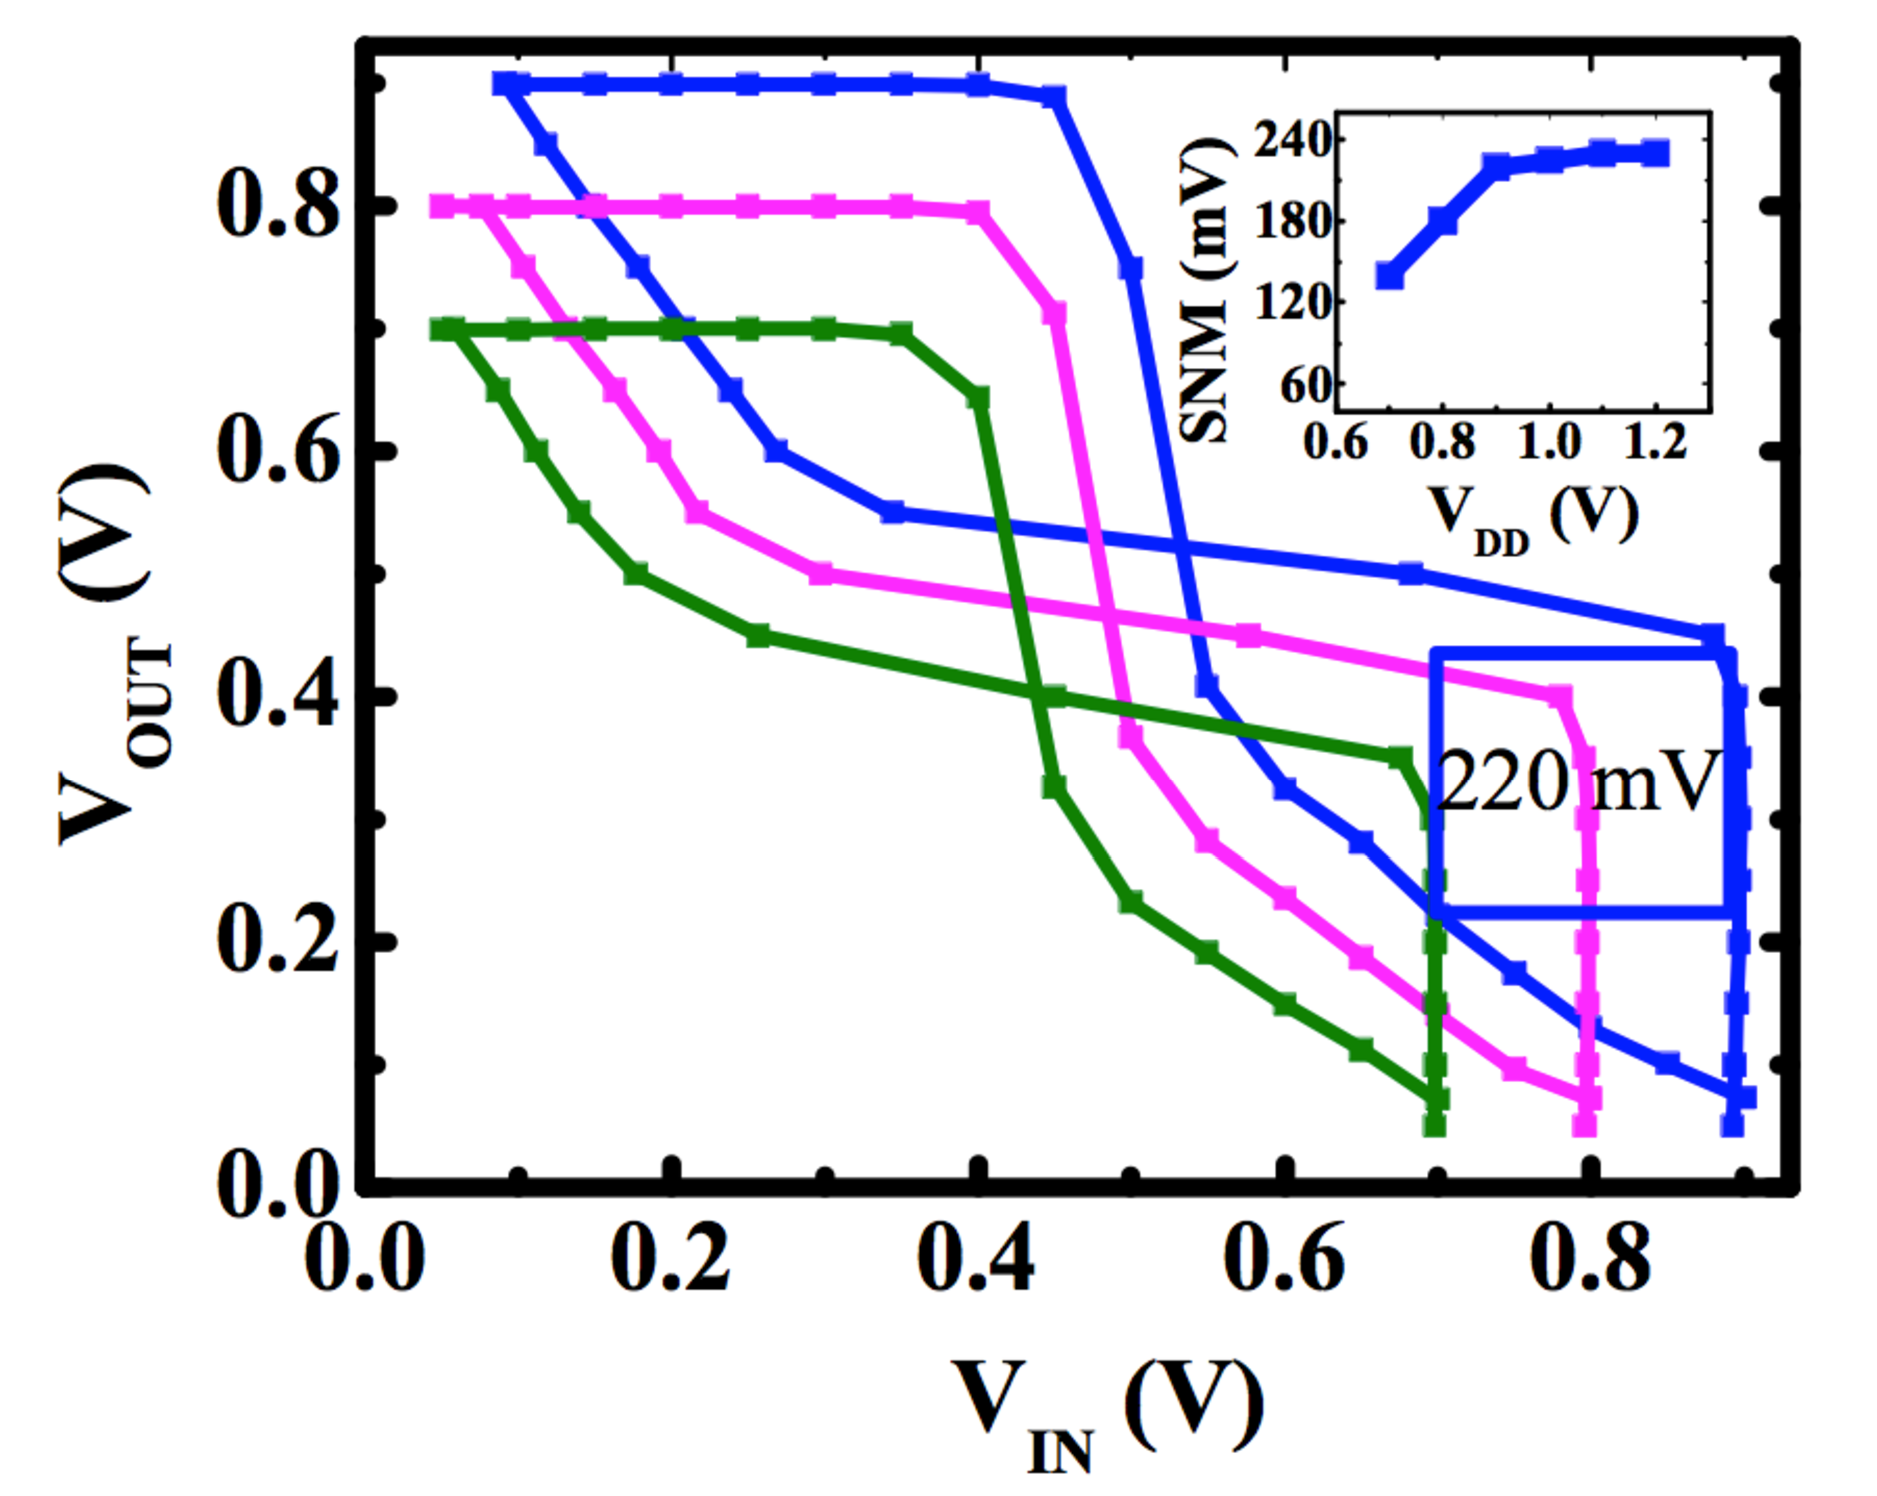
\includegraphics[width=5in]{haran_snm_butterfly_curves.pdf}
    \end{center}
    \caption[Butterfly curves for 0.1 $\mu$m$^2$ 6T-SRAM cell showing SNM of 220~mV, 180~mV and 148~mV at V$_{dd}$=0.9, 0.8 and 0.7~V respectively.]{Butterfly curves for 0.1 $\mu$m$^2$ 6T-SRAM cell showing SNM of 220~mV, 180~mV and 148~mV at V$_{dd}$=0.9, 0.8 and 0.7~V respectively \cite{Haran:2008ta}.}
    \label{fig:22nm_soi_sram_butterfly_curve_snm}
\end{figure}

Fig.~\ref{fig:22nm_soi_sram_butterfly_curve_snm} shows the transfer characteristics, also known as butterfly curves, for a functional 22~nm SOI SRAM from \cite{Haran:2008ta}.
The transfer characteristics represent the input/output states of the two cross coupled inverters that comprise an SRAM cell.
Here $V_{in}$ is arbitrarily chosen to be the data state of $Q$ in Fig.~\ref{fig:SRAM_Cell} and $V_{out}$ represents the output value $\overline{Q}$. 
When $V_{in}$ is high, the transistors $M_1$ and $M_2$ are in the off and on states, respectively, and the corresponding value of $V_{out}$ is low.
The value of $V_{out}$ is the input state of the inverter comprised of transistors $M_3$ and $M_4$. 
When $V_{out}$ is low, transistors $M_3$ and $M_4$ are in the on and off states, respectively, which reinforce a high state of $V_{in}$.
By sweeping $V_{in}$ from high to low the transistors $M_1$ and $M_2$ change to the on/off configuration, sending $V_{out}$ high which in turn forces the transistors $M_3$ and $M_4$ into the off/on configuration.

The stability of an SRAM cell is generally described in terms of the static noise margin (SNM), which is the \emph{DC} noise an SRAM cell can tolerate while maintaining its intended state.
The SNM of an SRAM cell is the side-length, given in millivolts, of the largest inscribed square that fits between the $V_{in}$/$V_{out}$transfer characteristics of Fig.~\ref{fig:22nm_soi_sram_butterfly_curve_snm}.
Exceeding the SNM for an SRAM cell results in a change of information state.
Three sets of transfer characteristics are shown in Fig.~\ref{fig:22nm_soi_sram_butterfly_curve_snm}, corresponding to supply voltages of 0.9~V (blue curves), 0.8~V (pink curves), and 0.7~V (green curves).
Fig.~\ref{fig:22nm_soi_sram_butterfly_curve_snm} shows the SNM of an SRAM cell depends on the supply voltage, with lower $V_{DD}$ corresponding to a smaller SNM.
Similarly, the switching voltage, the input voltage where the state of the SRAM cell changes from a \emph{1} to \emph{0}, or vice versa, also depends on the supply voltage.
The decrease in switching voltage and SNM under reduced supply voltage conditions effectively increases the sensitivity of SRAM cells to errors from dynamic disturbances caused by ionizing radiation, crosstalk, supply voltage ripple, and thermal noise.
% section basic_sram_topology_and_operation (end)

\section{Radiation Effects on SRAMs} % (fold)
\label{sec:radiation_effects_on_sram}
This section discusses the effects of radiation on SRAMs. 
Much of this section focuses on the concept of to SEUs with an emphasis on understanding the circuit-level response.
The concept of critical charge is defined for the purpose of understanding the methods and analysis in Chapters \ref{cha:experimental_investigation_of_electron_induced_seus} and \ref{ch:simulation_of_electron_induced_seus}.
Recent studies describing the observation of low-energy proton- and muon-induced upsets and the impact of those results for microelectronics will be discussed, emphasizing the trend towards increased sensitivity in modern devices. 
The effects of TID on SRAMs will be introduced with the primary example being the ``memory pattern imprinting'' effect. 
Relevant issues related to transient radiation environments, so-called dose-rate effects, will also be discussed.

\subsection{Single-Event Upset in SRAMs} % (fold)
\label{sub:single_event_upset_in_srams}
Energetic particles passing through material lose energy through electronic and nuclear processes as discussed in Sections~\ref{sub:ion_transport} and \ref{sub:electron_transport}. 
The electronic component consists of energy loss due to interaction with valance band electrons in the target material. 
Energy loss by the incident ion results in generation of mobile carriers in the conduction band and valance band, known as \emph{e-h} pairs.
Generated \emph{e-h} pairs are collected through the drift carrier transport process, resulting in a transient on affected semiconductor junctions.
Carriers generated in field free regions either recombine or diffuse to nearby regions where they are collected by electric fields, contributing to transients on adjacent terminals.

The physics of radiation-induced charge collection in semiconductor devices is a complicated topic and has been well-studied and reviewed in \cite{mclean1982charge,oldham1983charge,oldham1986revised,dodd1994three,edmonds1997charge,edmonds1998electric,hubert2000study,edmonds2010theoretical,edmonds2011proposed,edmonds2011theoretical,edmonds2011extension,hooten2012significance}.
Collection of \emph{e-h} pairs due to the presence of electric fields, known as drift current, diffusion of carriers in high-level injection regions into nearby junctions, and modulation of local potentials due to the resulting transients all play significant roles in the response of semicondcutor devices to single ionizing particle events.
By their nature, ionizing particle events generate dense regions of charge in the spatial locations where they interact making it difficult to represent the device response without the aid of computer tools, such as SPICE \cite{gadlage2004single,kauppila2009bias,massengill:1993sc} and TCAD \cite{dodd1994three,dasgupta2007effect,massengill:1993sc}.

The amount of charge generated by the passage of a incident ion through a sensitive region of a semiconductor memory is related to the average energy required to generate a single \emph{e-h} pair, in silicon this energy is 3.6~eV.
In this sense, the energy lost by an incident particle is correlated with the amount of charge generated within the semiconductor device material.
The \emph{effective} area defining the sensitive region of an SRAM cell is expressed in terms of a SEU cross-section.
The cross-section represents a region where ionizing particles that interact with the target material may perturb circuit-level operation and potentially  cause an error in memory.
Upset cross-sections are represented by the symbol $\sigma$ and typically given in units of cm$^2$/bit or cm$^2$/Mbit.
SEU cross-sections have typically been analyzed as a function of incident ion LET based on the assumption that knowledge of the average interaction is sufficient to predict the event response, and subsequently, the error rate in the environment of interest.

\begin{figure}[htbp]
    \begin{center}
        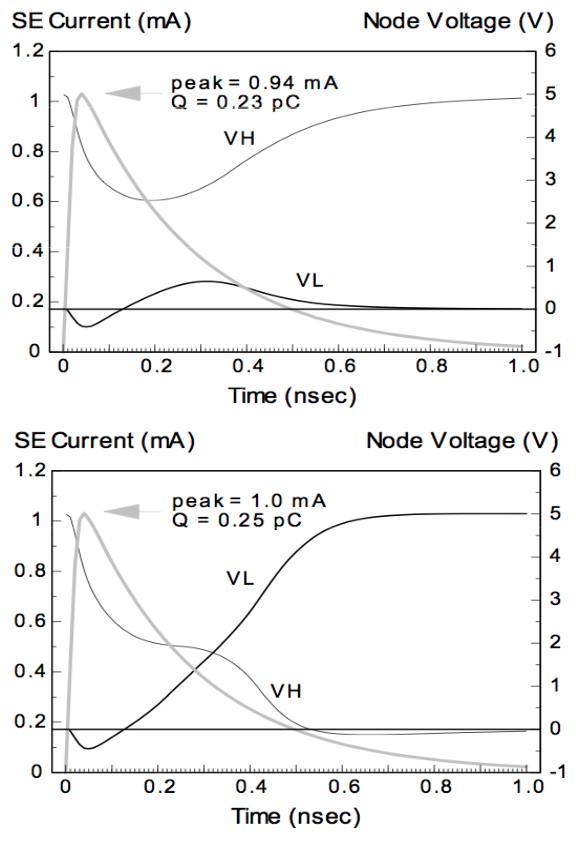
\includegraphics[width=4in]{qcrit_concept.pdf}
    \end{center}
    \caption[Current transients in an SRAM cell demonstrate the concept of critical charge. The transient corresponding to 0.23~pC of charge collection is insufficient to cause the SRAM cell to latch into an erroneous state. However, when the amount of collected charge is increased to 0.25~pC the resulting transient is latched into the SRAM cell, resulting in an error.]{Current transients in an SRAM cell demonstrate the concept of critical charge. The transient corresponding to 0.23~pC of charge collection is insufficient to cause the SRAM cell to latch into an erroneous state. However, when the amount of collected charge is increased to 0.25~pC the resulting transient is latched into the SRAM cell, resulting in an error \cite{massengill:1993sc}.}
    \label{fig:qcrit_concept}
\end{figure}

As an \emph{example}, Fig.~\ref{fig:qcrit_concept} demonstrates the concept of critical charge, which is defined as the charge required to induce an upset in an SRAM cell \cite{massengill:1993sc}.
Two transients are shown in Fig.~\ref{fig:qcrit_concept} with different amounts of total charge being collected and the resulting transient on the output of the off-state transistor in an SRAM cell.
The top image of Fig.~\ref{fig:qcrit_concept} shows a transient corresponding to 0.23~pC of charge collection within the SRAM cell.
The state of the cell is temporarily perturbed, however, the resulting transient is insufficient to cause the SRAM cell to latch into an erroneous information state.

In the bottom image of Fig.~\ref{fig:qcrit_concept}, the transient shown corresponds to 0.25~pC of charge collected in the SRAM cell. 
While the magnitude of charge collection differs by only 0.02~pC, the resulting circuit response is dramatically different. 
The resulting transient is of sufficient magnitude and duration to latch an erroneous state into the SRAM cell, resulting in an externally visible error.
The critical charge of this SRAM cell would therefore be defined to be 0.25~pC since a typical SRAM cell response for the corresponding technology node  would result in an error.

There are many nuances and specific details that may impact the error margins for determining critical charge such as corner to corner variations, magnitude and duration of the transient pulse, and charge collection efficiency \cite{Warren:2007vm,Warren:2007ca,kauppila2009bias,kauppila2011pvsram,kauppila2011pvcs}. 
However, Fig.~\ref{fig:qcrit_concept} is intended solely to convey the concept of critical charge, which is defined in this dissertation as a single valued metric for determining the energy deposition threshold for the onset of errors in an SRAM cell.
We will see that the magnitude of charge collection shown in Fig.~\ref{fig:qcrit_concept} is extremely large when compared to the critical charge for sub-65~nm technology nodes as discussed in Chapters~\ref{cha:experimental_investigation_of_electron_induced_seus} and \ref{ch:simulation_of_electron_induced_seus}.

The first attempts to quanitfy the critical charge of SRAMs developed circuit models from known topologies and process information to be used in SPICE simulations \cite{buehler1990alpha,roth1993monitoring}.
SPICE simulations were performed using double exponential current pulses to emulate the current transient response of an SRAM cell and evaluate whether cells were likely to upset, this methodology has proven very robust over the years and is still commonly used.
In a similar fashion, Buehler \emph{et al.} used this SPICE simulation technique and analysis to show the SRAM cell critical charge dependence on supply voltage, those results are shown in Fig.~\ref{fig:qcrit_vdd_dep} \cite{buehler1990alpha}.
Small decreases in supply voltage are shown to result in linear modulation of the SRAM cell critical charge.
This trend continues until a large discrepancy between applied and nominal supply voltage results in SRAM cell instability, causing spontaneous errors in the memory array as shown by the change in slope of Fig.~\ref{fig:qcrit_vdd_dep} around 1.9~V.
Understanding the lower limit of critical charge also informs regions of stable operation for an SRAM as the memory operates normally and maintains valid data for supply voltage conditions above this threshold.
While the magnitude of critical charge in Fig.~\ref{fig:qcrit_vdd_dep} is large compared to SRAMs fabricated in sub-65~nm technology nodes, the conceptual discussion above is still valid serves as an informative case study.
\begin{figure}[tb]
    \begin{center}
        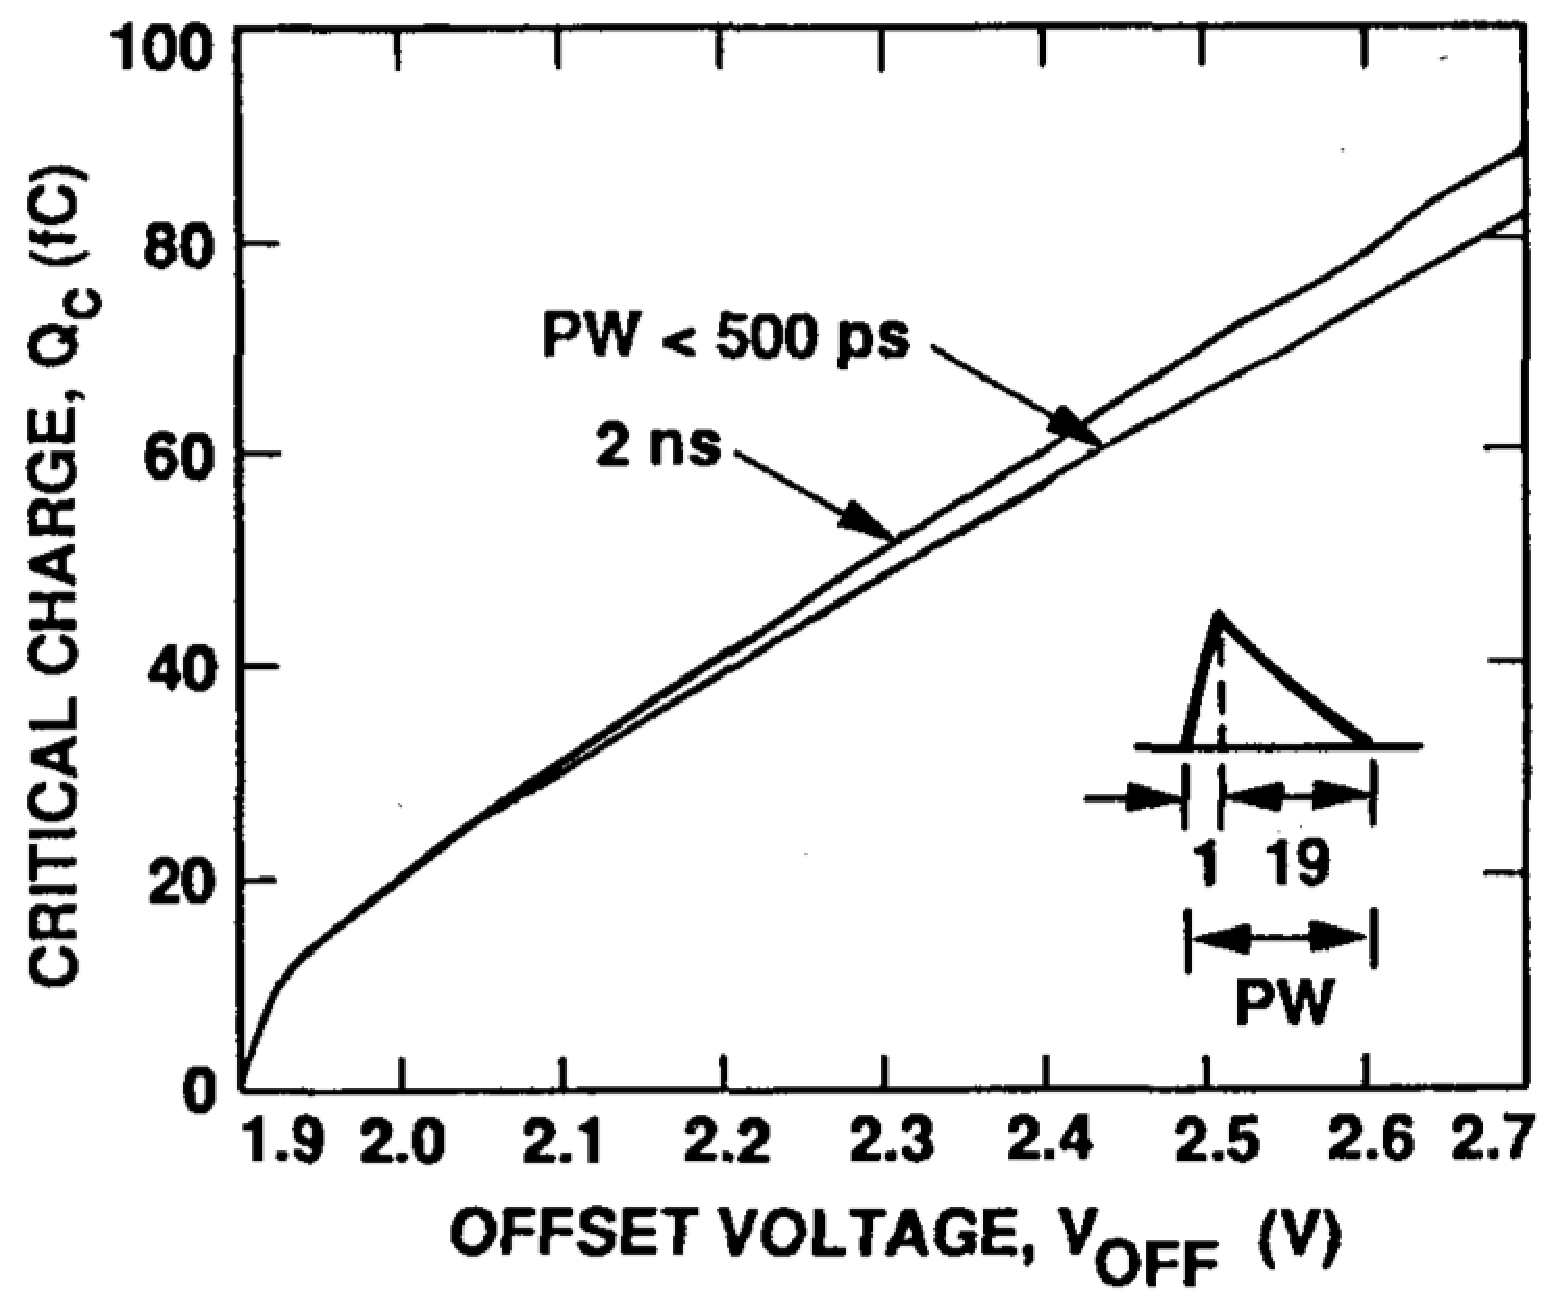
\includegraphics[width=5in]{buehler_qcrit_vdd_dep.pdf}
    \end{center}
    \caption[SPICE analysis of the critical charge dependence on supply voltage]
    {SPICE analysis an SRAM cell critical charge dependence on supply voltage from \cite{buehler1990alpha}.}
    \label{fig:qcrit_vdd_dep}
\end{figure}

The critical charge dependence of SRAMs on supply voltage is only one part of a complicated story.
In addition to the supply voltage, the SEU response also depends on the LET of the incident particle.
The SEU bias and LET dependence of SRAMs has been discussed previously in \cite{buehler1990alpha,barak1999scaling,barak2004use}.
In~\cite{barak2004use}, Barak \emph{et al.} used alpha particles to show the SEU cross-section bias dependence on supply voltage, those results can be seen in Fig.~\ref{fig:seu_vdd_dep}.
The SEU cross-sections shown in Fig.~\ref{fig:seu_vdd_dep} exhibit a clear exponential dependence on applied bias.
Additionally, Fig.~\ref{fig:seu_vdd_dep} shows a dependence on the incident ion LET.
Higher LET alpha particles are observed to have a higher cross-section under large applied bias conditions as compared to lower LET alpha particles.
Higher LET alpha particles also exhibit a non-uniform slope in corresponding SEU cross-sections.
This is because continued reduction in supply voltage modulates the critical charge below the average charge generated within the sensitive volume by the incident alpha particles, which in turn results in only a moderate increase in the measured cross-section.
Due to the low onset voltage for more lightly ionizing particles, this feature may be reduced or entirely absent from the SEU cross-section versus supply voltage figures as shown by the lower LET alphas (5.49~MeV) in Fig.~\ref{fig:seu_vdd_dep}.
These trends have also been shown in other works for heavy-ions, alphas, and low-energy protons in \cite{buehler1990alpha,barak1999scaling,barak2004use,Rodbell:2007vl,Heidel:2008vf}.
\begin{figure}[tb]
    \begin{center}
        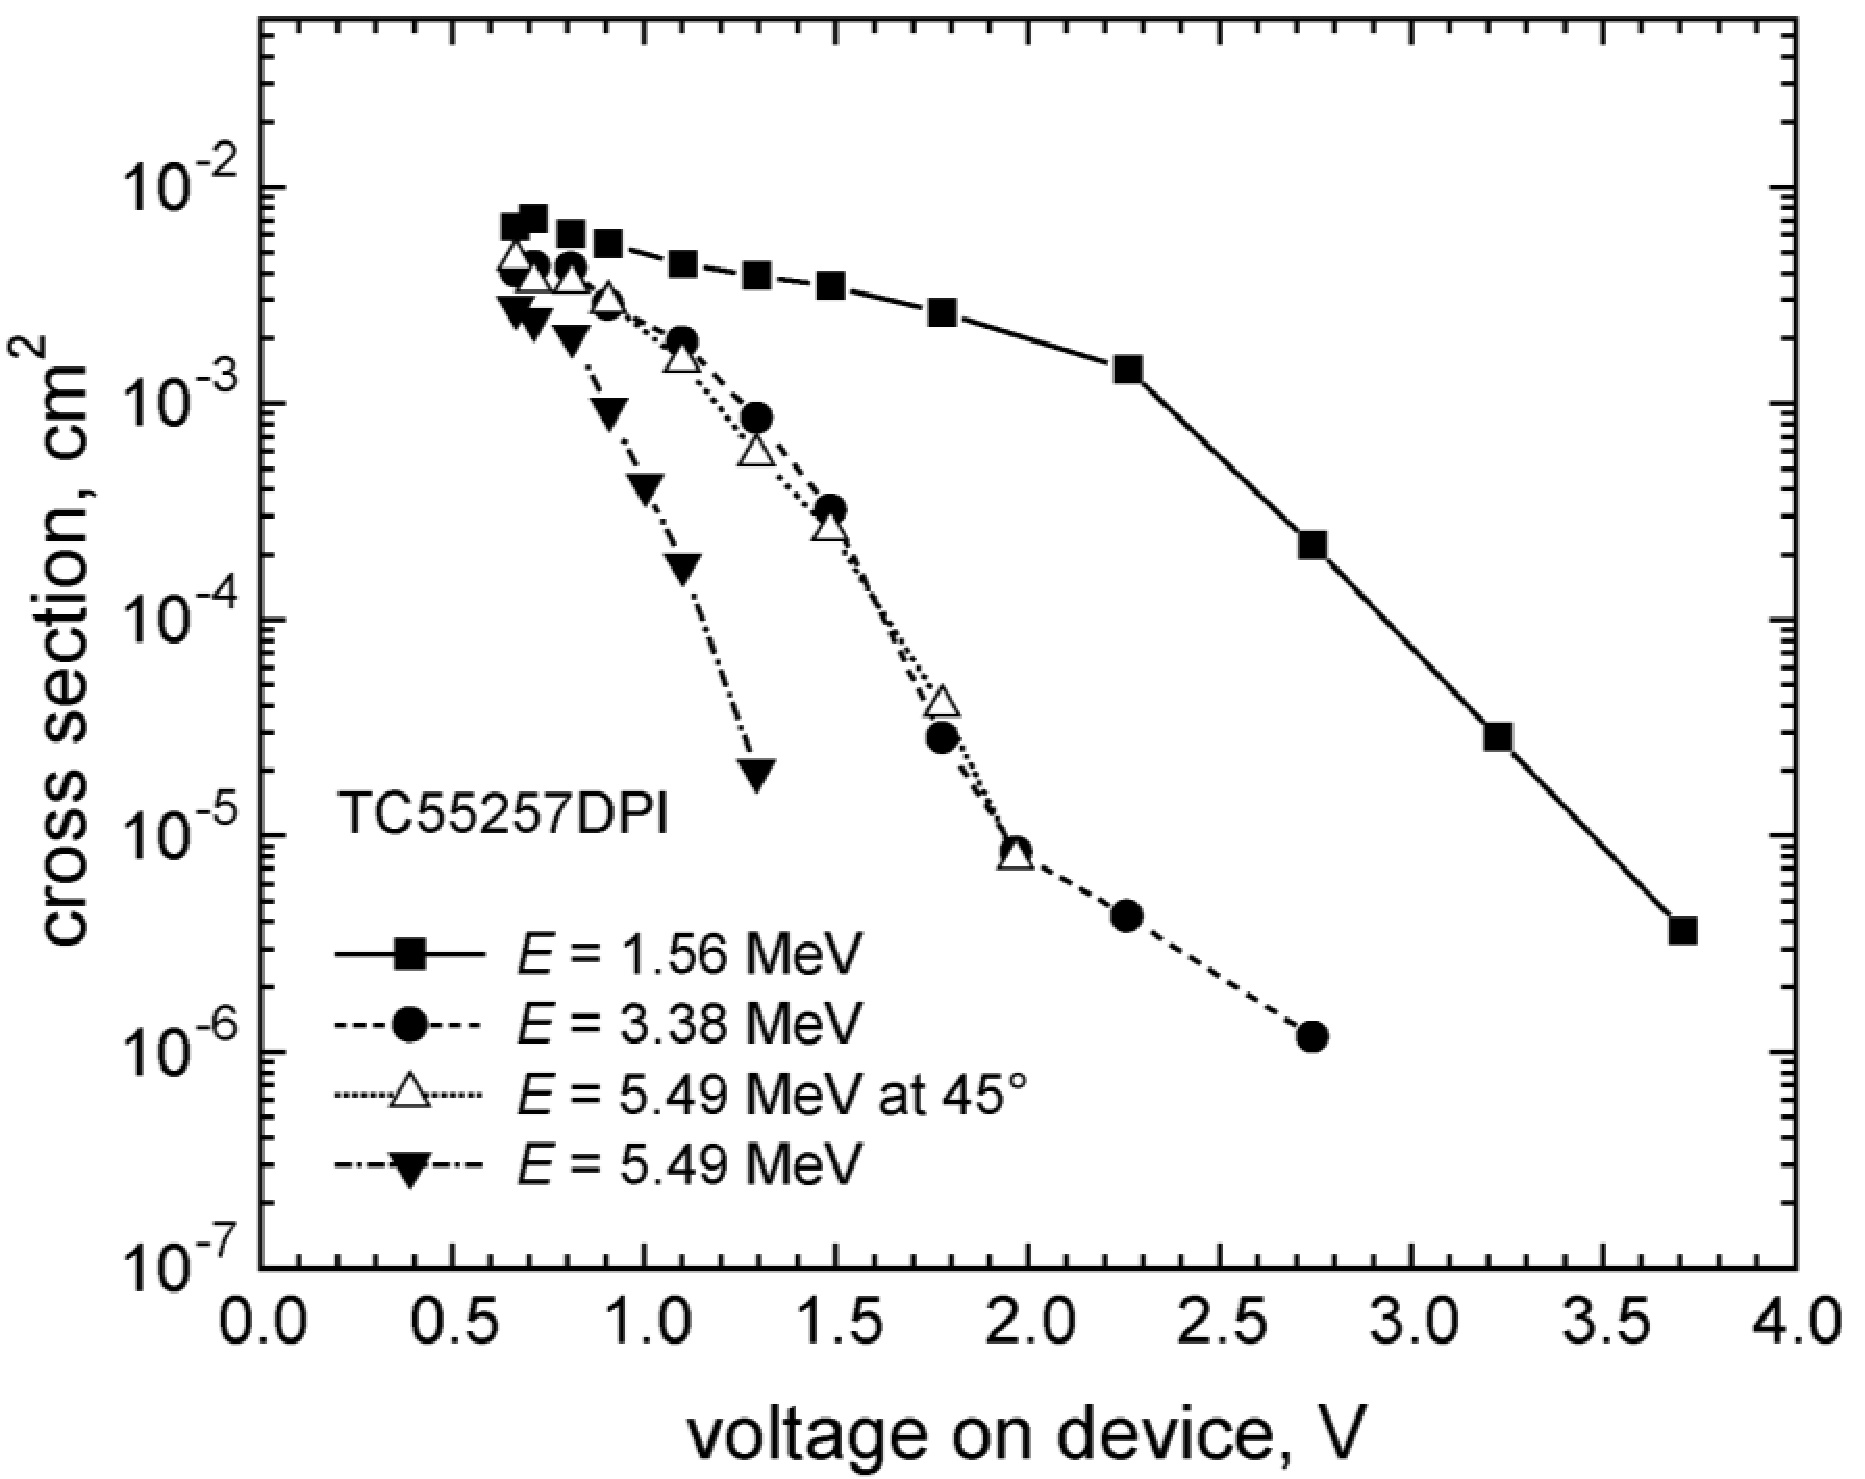
\includegraphics[width=5in]{barak_seu_bias_dep_2.pdf}
    \end{center}
    \caption[SEU cross-section bias dependence of an SRAM for alphas with energies 1.56, 3.38, and 5.49~MeV, with LETs (in the sensitive volume) of 1.52, 0.87, and 0.64~MeV-cm$^2$/mg, respectively.]
    {SEU cross-section bias dependence of an SRAM for alphas with energies 1.56, 3.38, and 5.49~MeV, with LETs (in the sensitive volume) of 1.52, 0.87, and 0.64~MeV-cm$^2$/mg, respectively. After \cite{barak2004use}.}
    \label{fig:seu_vdd_dep}
\end{figure}

\begin{figure}[tb]
    \begin{center}
        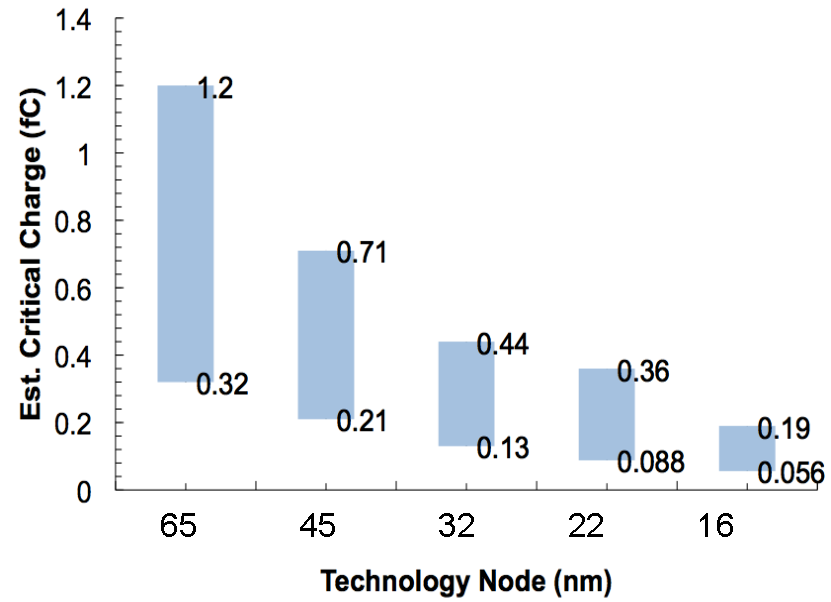
\includegraphics[width=5in]{qcrit_trends.pdf}
    \end{center}
    \caption[Estimation of critical charge as a function of technology node feature size.]
    {Estimation of critical charge as a function of technology node feature size \cite{Sierawski:2011tc}.}
    \label{fig:qcrit_trends}
\end{figure}
In \cite{Sierawski:2011tc}, Sierawski attempted to estimate the critical charge for several current- and next-generation technology nodes, the resulting calculations can be seen in Fig.~\ref{fig:qcrit_trends}.
Using SPICE simulations and injecting current pulses of varying magnitude and duration Sierawski was able to obtain an upper bound for critical charge.
The lower bounds were obtained by extracting process details from the ITRS road map \cite{itrs:2012} and applying the following relation,
\begin{equation}
    \label{eq:qcrit}
    Q_{crit} = \frac{V_{DD}}{2}\frac{\epsilon_{SiO_2} \epsilon_0 A_{cell}}{t_{ox}}
\end{equation}
where $V_{DD}$ is the supply voltage for the technology node, $\epsilon_{0}$ is the permittivity of free space, $\epsilon_{SiO_2}$ is the relative permittivity of SiO$_2$, $A_{cell}$ is the cell area, and $t_{ox}$ is the equivalent SiO$_2$ oxide thickness for the technology node.
Fig.~\ref{fig:qcrit_trends} shows an overall decrease in critical charge with decreasing technology node feature size.
These conclusions are consistent with publications that indicate the critical charge of 65~nm silicon-on-insulator SRAMs is between 0.21 and 0.27~fC \cite{Rodbell:2007vl}.

%   Some of this seems to need to go into a different section
While much of the energy lost by the incident ion results in the generation of \emph{e-h} pairs by direct ionization, secondary particles also deposit energy in regions surrounding the incident ion path and have been reported to contribute to the SEU response.
The secondary particles of concern are generated by incident particles through nuclear elastic, inelastic or spallation reactions, or Coulomb scatters, known as ``knock-ons,'' which are atoms displaced from the crystal lattice.
Several studies have investigated the fidelity of electron, or $\delta$-ray, induced SEUs with mixed conclusions.
Some reports indicate that $\delta$-rays may contribute to the overall single- and multiple-bit upset cross-section in a heavy-ion environment \cite{King:2010cu,King:2012cb}.
Others have found that any contribution from $\delta$-rays in such an environment does not contribute significantly to a measureable upset cross-section \cite{Raine:gk,Raine:2012gi,Barak:2012im}.
The generation and interactions of $\delta$-rays in a heavy-ion environment will be discussed thoroughly in Section~\ref{sec:evaluating_track_structure}.
This dissertation will demonstrate SEUs for SRAMs exposed to a source of electrons and investigate the significance and contribution of electron induced SEUs to error-rates in the space radiation environment.
% subsection single_event_upset_in_srams (end)

\subsection{Low-Energy Proton-Induced SEUs} % (fold)
\label{sub:low_energy_proton_induced_seus}
The primary effects due to incident protons on microelectronics in the space radiation environment have historically been displacement damage, TID, and SEUs caused by nuclear spallation reactions \cite{reed1994implications,reed1997heavy,reed2002evidence,Reed:2007vz}.
The contribution of protons to upset cross-sections due to direct ionization has traditionally been ignored since the electronic stopping power of protons is quite small.
However, a series of papers demonstrated protons near their end of range were capable of generating sufficient charge to upset SRAMs and latches fabricated in a 65~nm node \cite{Heidel:2006tp,Heidel:2008vf,Heidel:2009vx,Rodbell:2007vl,Sierawski:2009ka}.

\begin{figure}[htbp]
    \begin{center}
        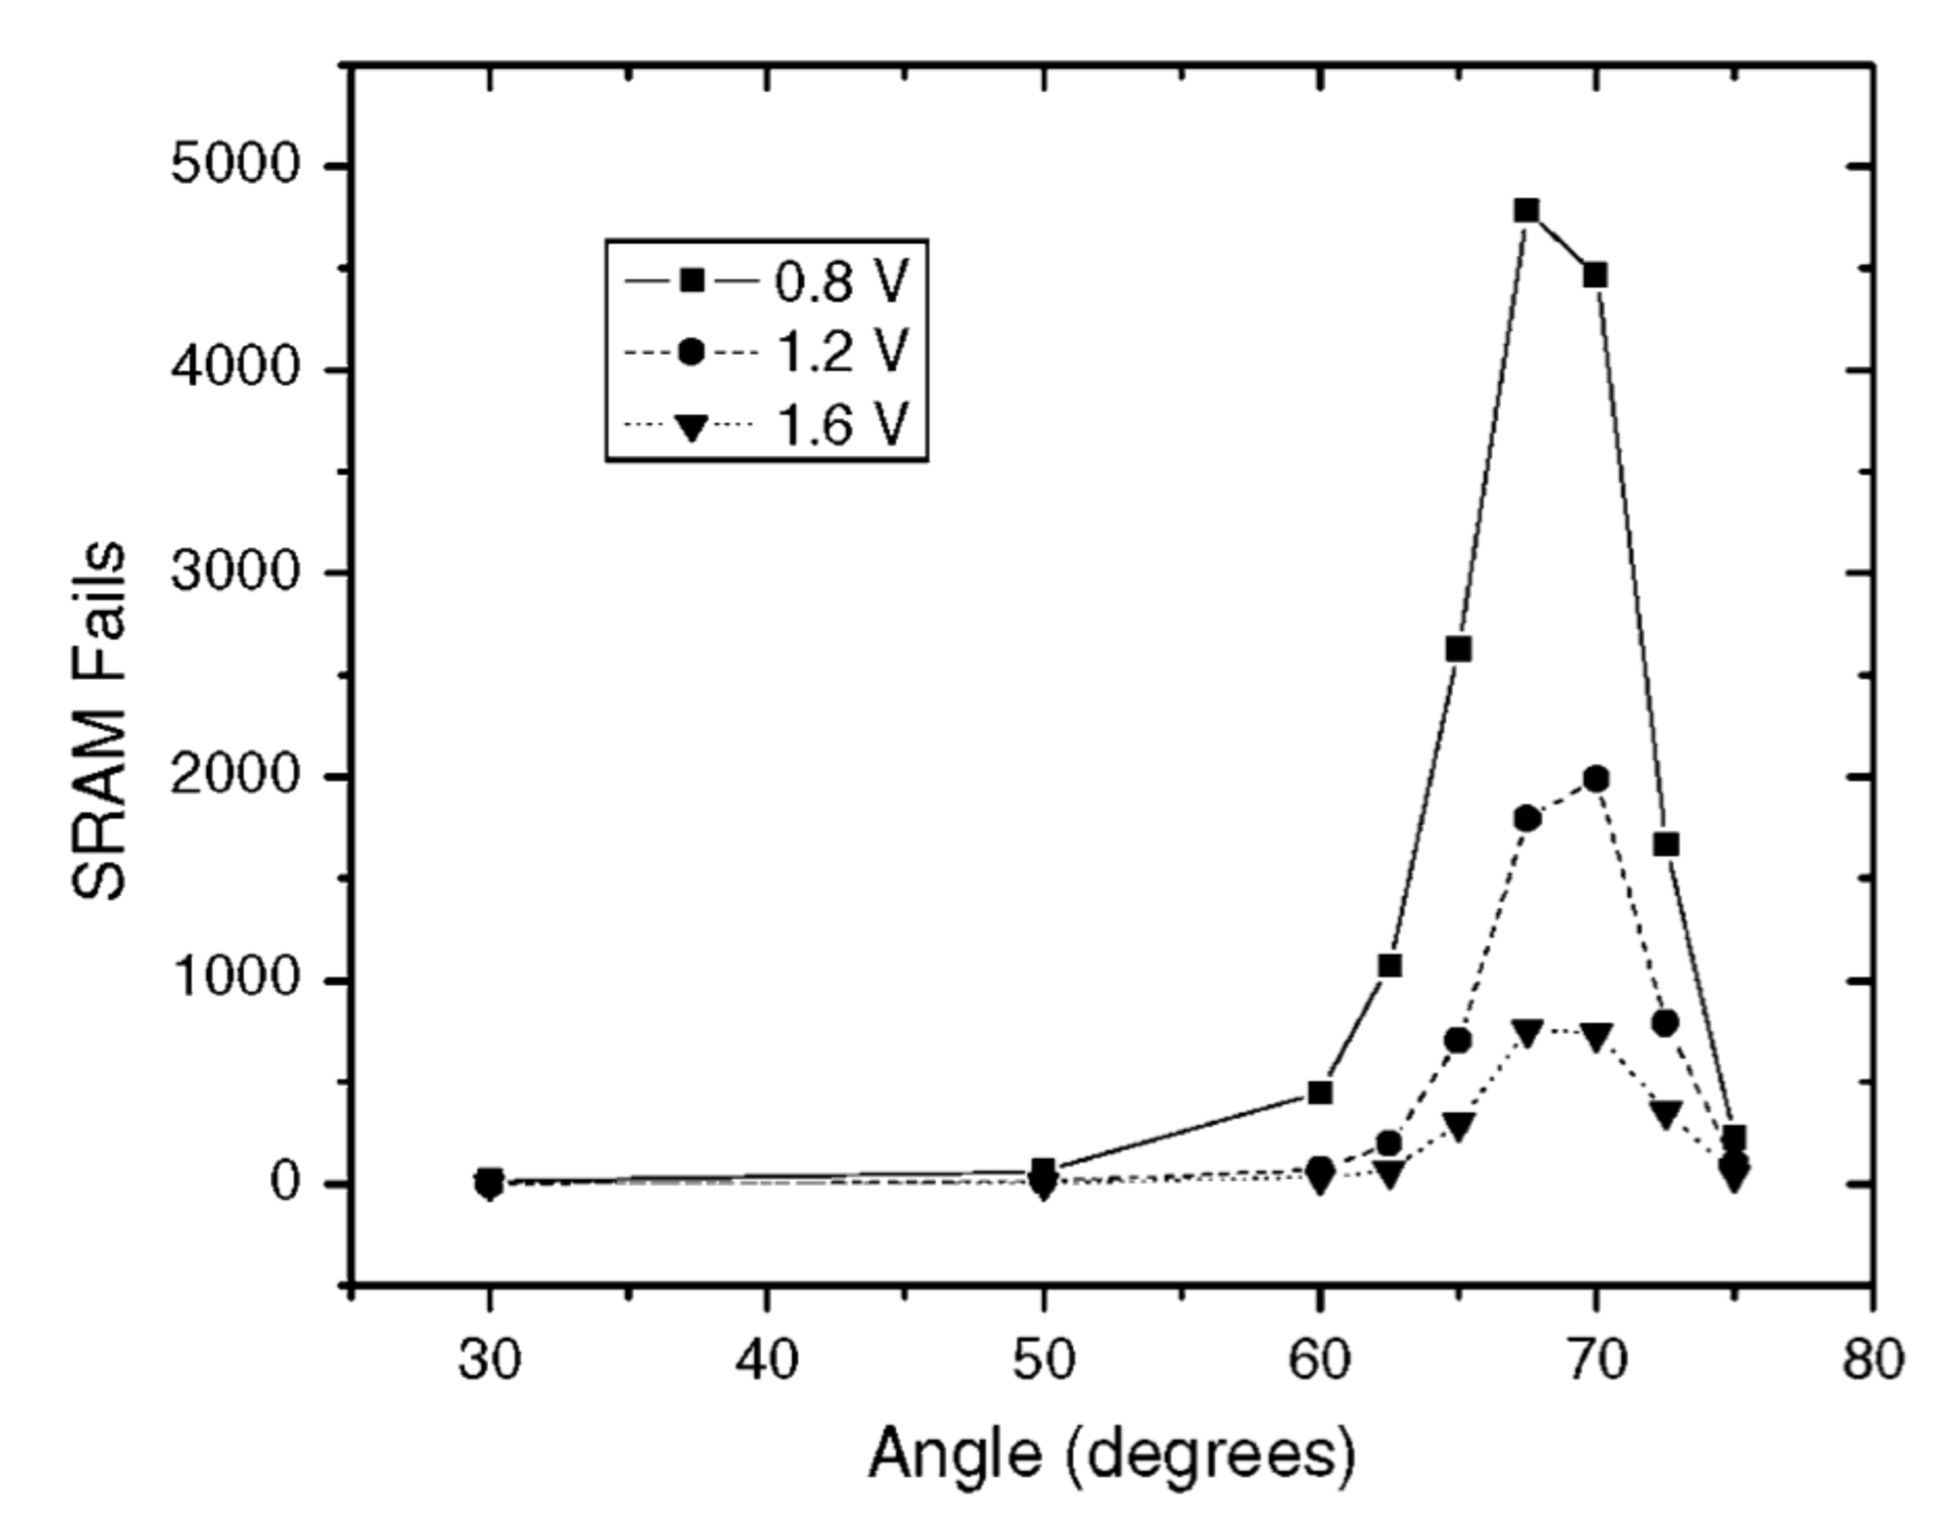
\includegraphics[width=5in]{sram_cell_failures_proton_angle.pdf}
    \end{center}
    \caption[SRAM fails (an average of write \emph{1} and write \emph{0}) as a function of the incident angle for an SRAM array at 0.8~V, 1.2~V and 1.6~V using 1.5~MeV protons.]{SRAM fails (an average of write \emph{1} and write \emph{0}) as a function of the incident angle for an SRAM array at 0.8~V, 1.2~V and 1.6~V using 1.5~MeV protons \cite{Rodbell:2007vl}.}
    \label{fig:sram_proton_angle_dep}
\end{figure}

The Bragg peak for protons occurs near their end of range, implying that protons near stopping have a maximum LET.
By exposing SRAM and latches to a source of low-energy protons, in the energy range of 1-2~MeV, Heidel and Rodbell were able to show that proton-induced direct ionization can cause upsets in SRAMs fabricated in 45~nm and 65~nm technology nodes \cite{Heidel:2006tp,Rodbell:2007vl,Heidel:2009vx}.
Because SOI technology has a large angular dependence \cite{Reed:2002wn}, proton direct ionization effects were confirmed by performing experiments at large angle of incidence.
Rotating parts using a goniometer in order to test parts at large angle of incidence, where a beam normally incident on the device under test is considered to be 0$^\circ$, resulted in an increased upset rate.
This is due to an increased path length for incident protons through the active region of the test chip, corresponding to more energy deposited within the sensitive region of the the SRAM \cite{Heidel:2006tp}.

\begin{figure}[htbp]
    \begin{center}
        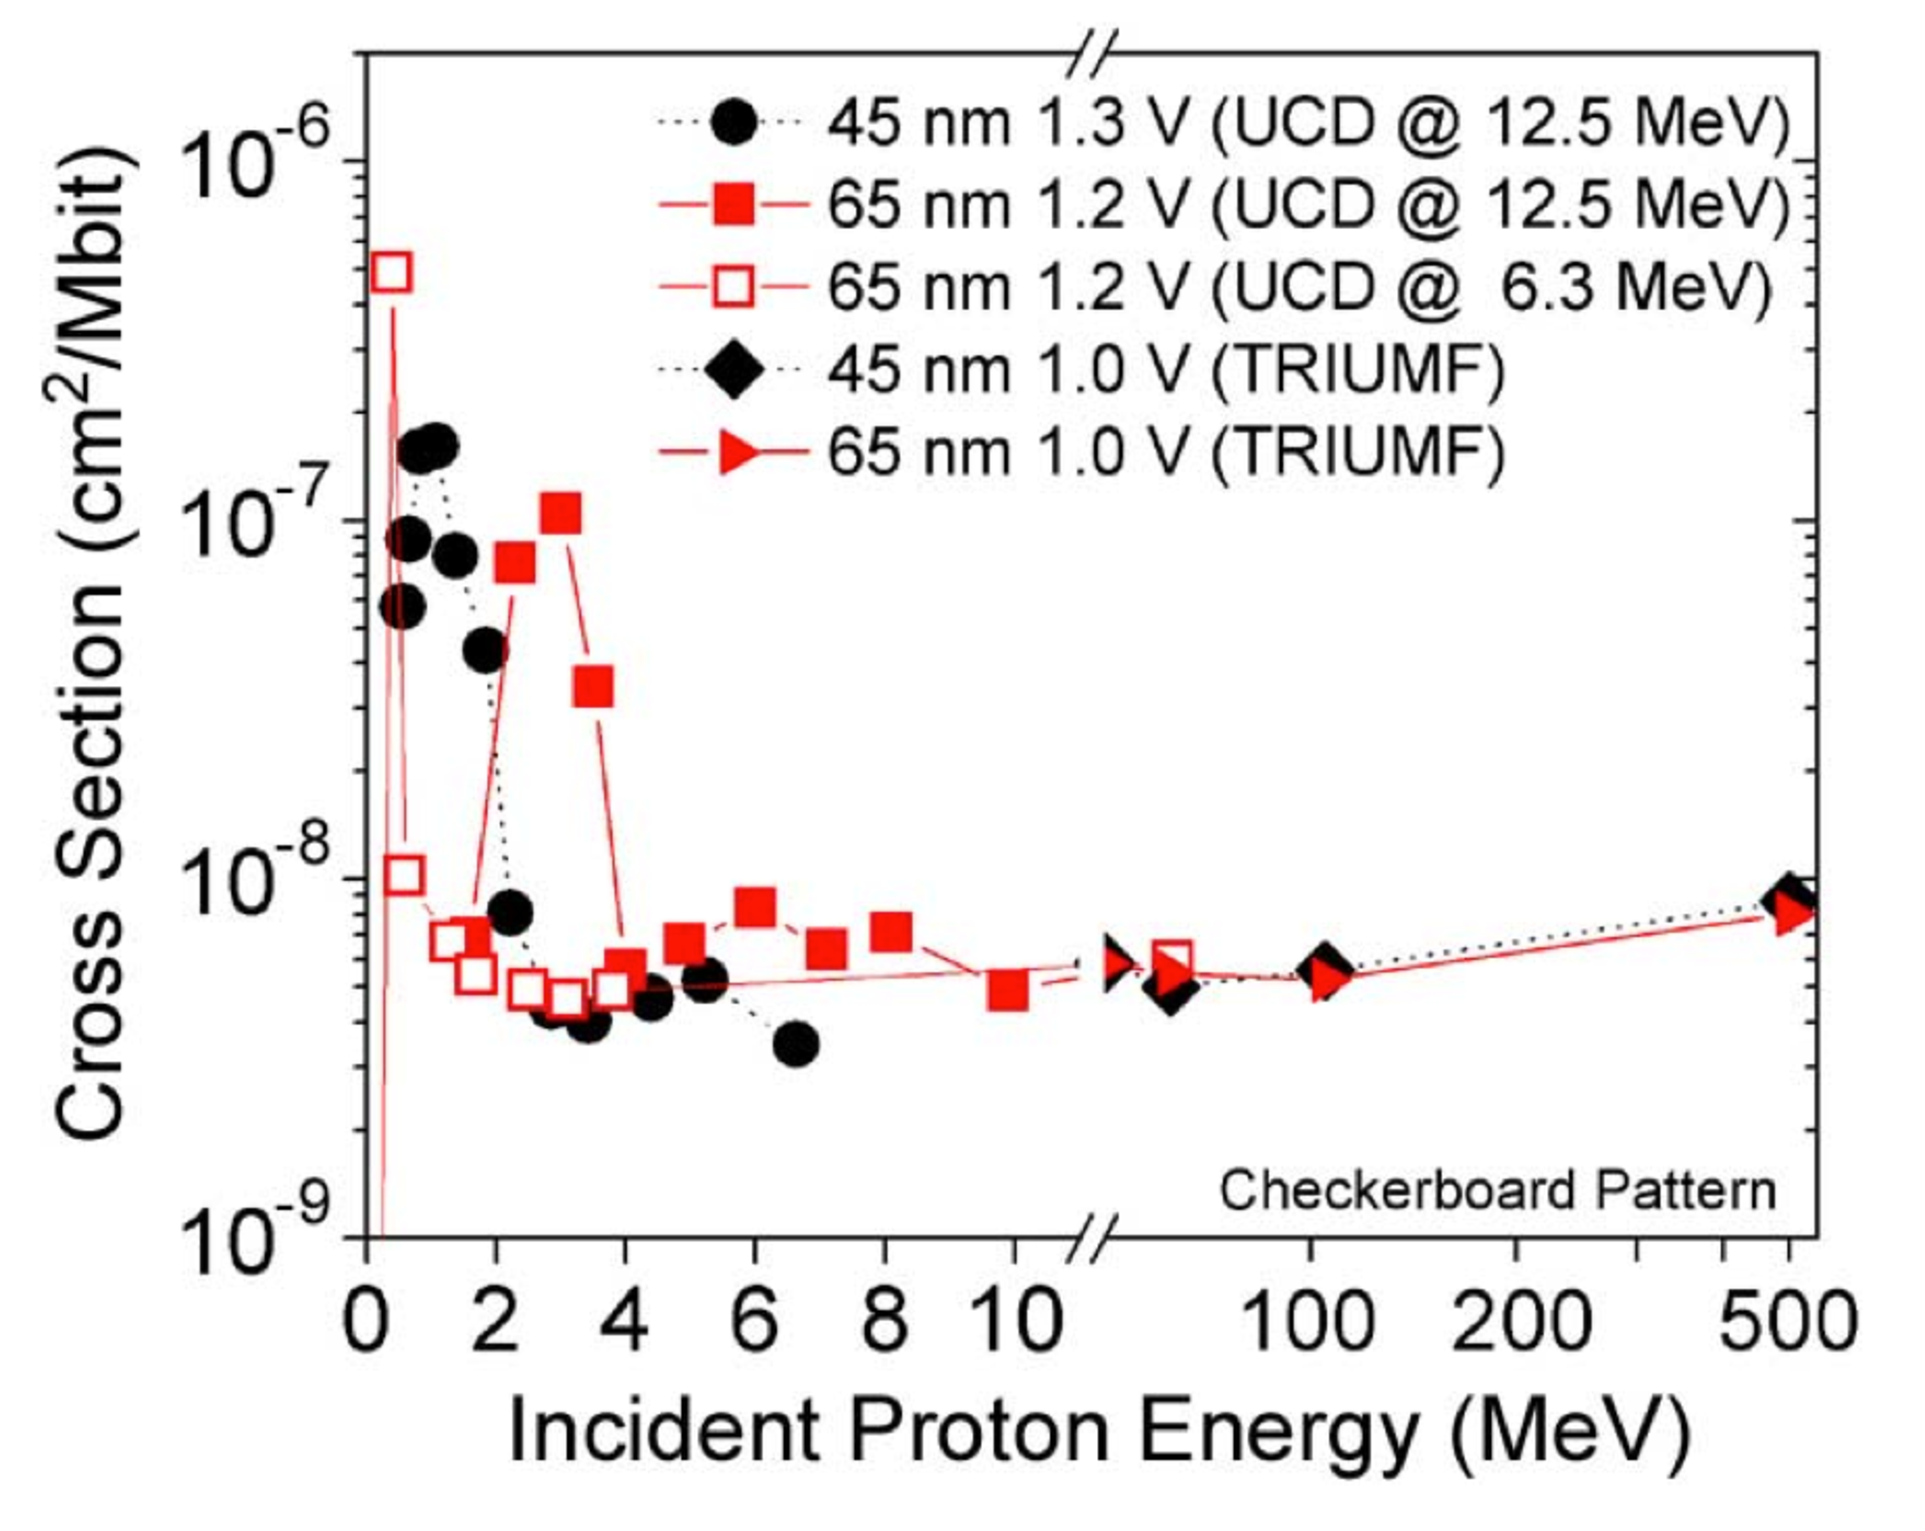
\includegraphics[width=5in]{proton_upset_cs_vs_energy.pdf}
    \end{center}
    \caption[The SBU cross section versus proton energy for both 45 nm and 65 nm SOI SRAMs.]{The SBU cross section versus proton energy for both 45 nm and 65 nm SOI SRAMs \cite{Heidel:2009vx}.}
    \label{fig:seu_cs_vs_p_energy}
\end{figure}

Fig.~\ref{fig:seu_cs_vs_p_energy} shows the proton SEU cross-section as a function of incident proton energy for 45~nm and 65~nm SRAMs.
For very energetic incident protons ($>$10~MeV) upsets can be attributed to nuclear reaction events.
In this energy range, the SEU cross-section remains fairly constant.
As the incident proton energy is reduced ($<$5~MeV) the measured upset cross-section begins to increase, corresponding to the protons with sufficient LET to upset the device under test.
Incident proton energies between 1-4~MeV correspond to a ``plateau'' in the measured upset cross-section.
In this region, the upset cross-section is two orders of magnitude higher than the high-energy proton cross-section and corresponds to a region where most of the incident protons are near their end of range.
Decreasing the incident proton energy further results in a reduced SEU cross section.
This is due to a corresponding reduction in the range of incident protons and prevents protons from transporting into the sensitive region of the device with sufficient energy to impact the SRAM cells nominal operation.

\begin{figure}[htbp]
    \begin{center}
        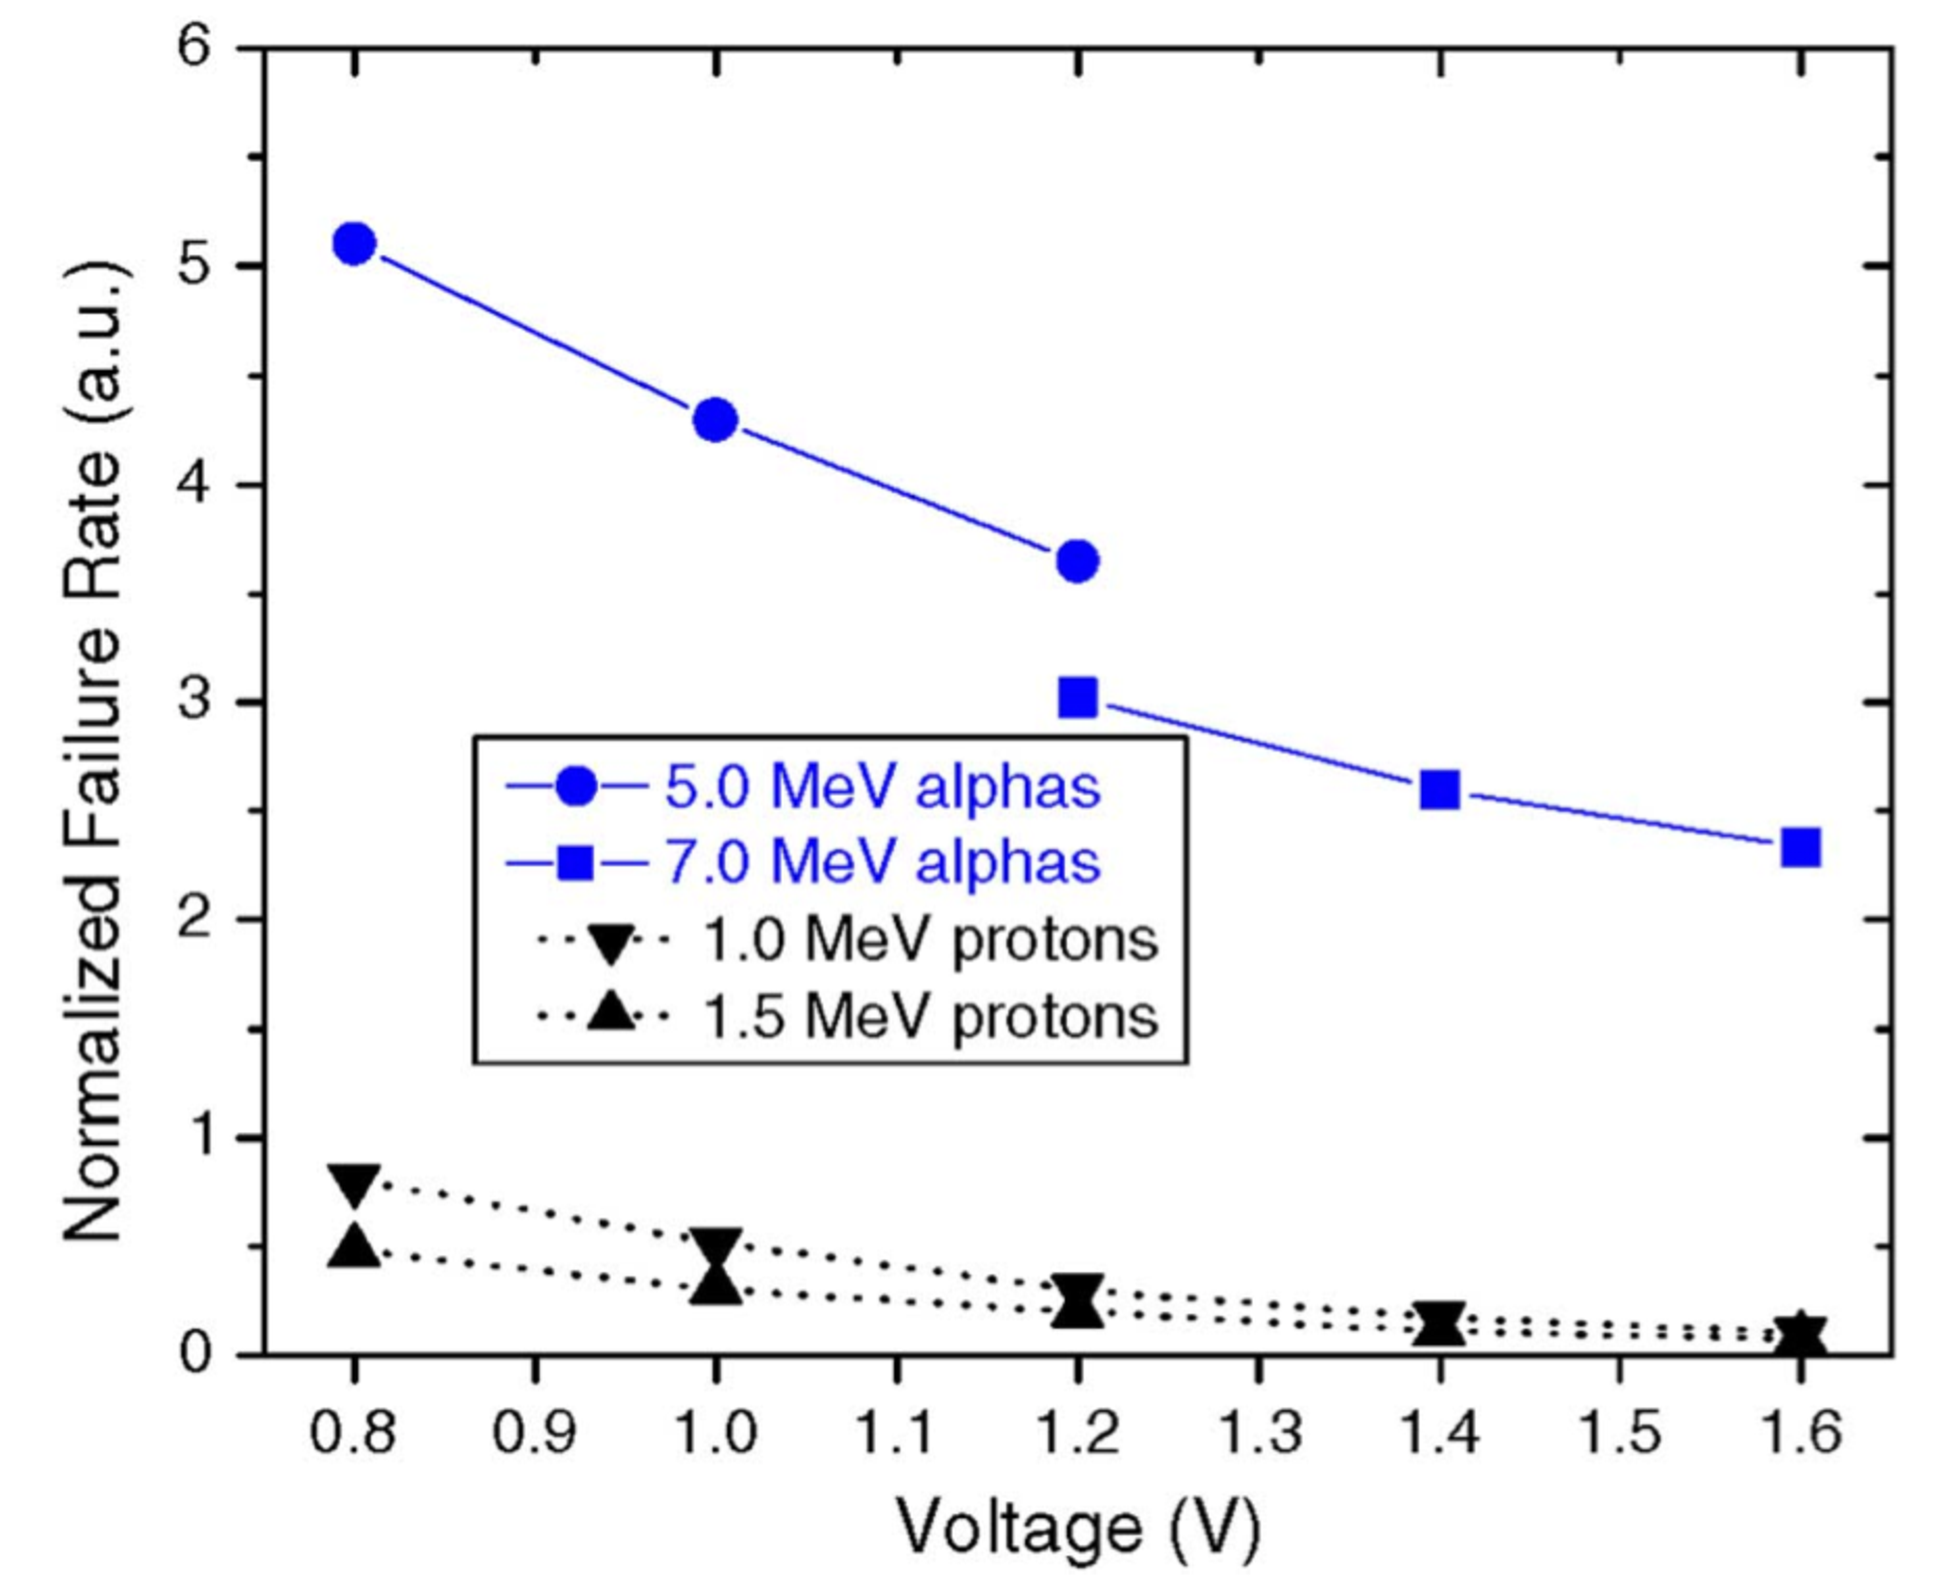
\includegraphics[width=5in]{65nm_sram_vdd_dep.pdf}
    \end{center}
    \caption[Plot of the SRAM SEU cross-section (in arbitrary units) as a function of voltage for 5.0~MeV and 7.0~MeV alpha particles and for 1.0~MeV and 1.5~MeV protons.]{Plot of the SRAM SEU cross-section (in arbitrary units) as a function of voltage for 5.0~MeV and 7.0~MeV alpha particles and for 1.0~MeV and 1.5~MeV protons \cite{Rodbell:2007vl}.}
    \label{fig:seu_cs_vs_appl_bias_protons}
\end{figure}

Closer study of Fig.~\ref{fig:seu_cs_vs_p_energy} shows that multiple supply voltage conditions were used while performing the initial low-energy proton experiments.
The sensitivity of SRAMs to low-energy protons was initially observed under reduced bias conditions at high angle of incidence \cite{Heidel:2006tp}.
Further study showed sensitivity of 45~nm SRAMs at normal incidence and under nominal bias conditions \cite{Rodbell:2007vl,Heidel:2009vx}.
A plot showing the SEU cross-section dependence on applied bias, in arbitrary units, can be seen in Fig.~\ref{fig:seu_cs_vs_appl_bias_protons} for 1~MeV and 1.5~MeV protons (also more energetic alpha particles are shown).
A gentle gradient can be observed in the SEU cross-section for low-energy protons (the curve corresponding to 1~MeV protons) as a function of applied bias.
Recalling the discussion regarding Eq.~\ref{eq:qcrit}, the critical charge of elementary 6T-SRAM cell should depend on the supply voltage \cite{buehler1990alpha,roth1993monitoring,barak1999scaling}.
In Fig.~\ref{fig:seu_cs_vs_appl_bias_protons}, the bias dependence manifests as a exponential slope in the measured SEU cross-section.
The SEU cross-section bias dependence is consistent with previous studies by Buehler \cite{buehler1990alpha} and Barak \cite{barak1999scaling,barak2004use} that show a dependence on both incident ion LET and supply voltage for SRAMs in several different technology generations.
Heidel and Rodbell both reported the critical charge for SRAMs fabricated in the 65~nm SOI technology node to have a critical charge between 0.21~fC and 0.27~fC \cite{Heidel:2006tp,Rodbell:2007vl}.
The values of critical charge from \cite{Heidel:2006tp,Rodbell:2007vl} are consistent with the estimations for SRAMs in the 65~nm technology node made by Sierawski and shown in Fig.~\ref{fig:qcrit_trends}.
Interestingly, the reported values of critical charge correspond to 1300-1700 collected electrons.
The observation of effects from low-energy protons signifies a noteworthy shift in the sensitivity of modern (here modern is taken to be sub-65~nm technology nodes) SRAMs.

These results primarily impact the device response to the space radiation environment, where energy loss through spacecraft shielding can shift the differential flux spectrum of protons towards lower energies, where direct ionization effects begin to contribute to the SEU cross-section and error rates \cite{Sierawski:2009ka}.
Nuclear reactions involving more energetic protons and/or the heavy ions from the galactic cosmic ray environment also result in the generation of large numbers of protons \cite{Rodbell:2007vl}.
The contribution of low-energy protons also extends to the terrestrial environment where neutron-induced spallation reactions produce a substantial number of low energy protons \cite{Rodbell:2007vl}.
% subsection low_energy_proton_induced_seus (end)

\subsection{Muon-Induced SEUs} % (fold)
\label{sub:muon_induced_seus}
Wallmark and Marcus performed a preliminary analysis of the fundamental limitations of microelectronics and highlighted ionizing radiation particles, chiefly amongst these were terrestrial muons and electrons, as the principal factors that would impact the continued reliable scaling of semiconductor devices and technology \cite{Wallmark:1962vn}.
Additional analysis regarding error rates and the sensitivity of SRAMs was performed by Ziegler \emph{et al.}
The results of that work suggested that the continued scaling of CMOS memory would result in a substantial increase in the sensitivity of SRAMs to ionizing radiation with continued device scaling and result in a large soft-error rate for the space and terrestrial radiation environments \cite{Ziegler:1979vh}.

As described in the previous section, research has shown commercial SRAMs are vulnerable to low-energy proton induced SEUs due to the relatively small critical charge required to cause an error in modern SRAMs.
This revelation has changed the way the radiation effects and reliability community view lightly ionizing radiation.
Contributions of low-energy protons to upset cross-sections, as discussed previously, were traditionally ignored, they are now being considered as a real and significant reliability concern.
For many years, the presence of atmospheric neutrons and alpha particles (largely the result of packaging impurities) presented the only feasible source of soft errors at the terrestrial level.
Muons, the most abundant species at the terrestrial level, have recently been shown to induce SEU in sub-65~nm SRAMs \cite{Sierawski:2010cj,Sierawski:2011tc,Sierawski:2011bn}.

\begin{figure}[tb]
    \begin{center}
        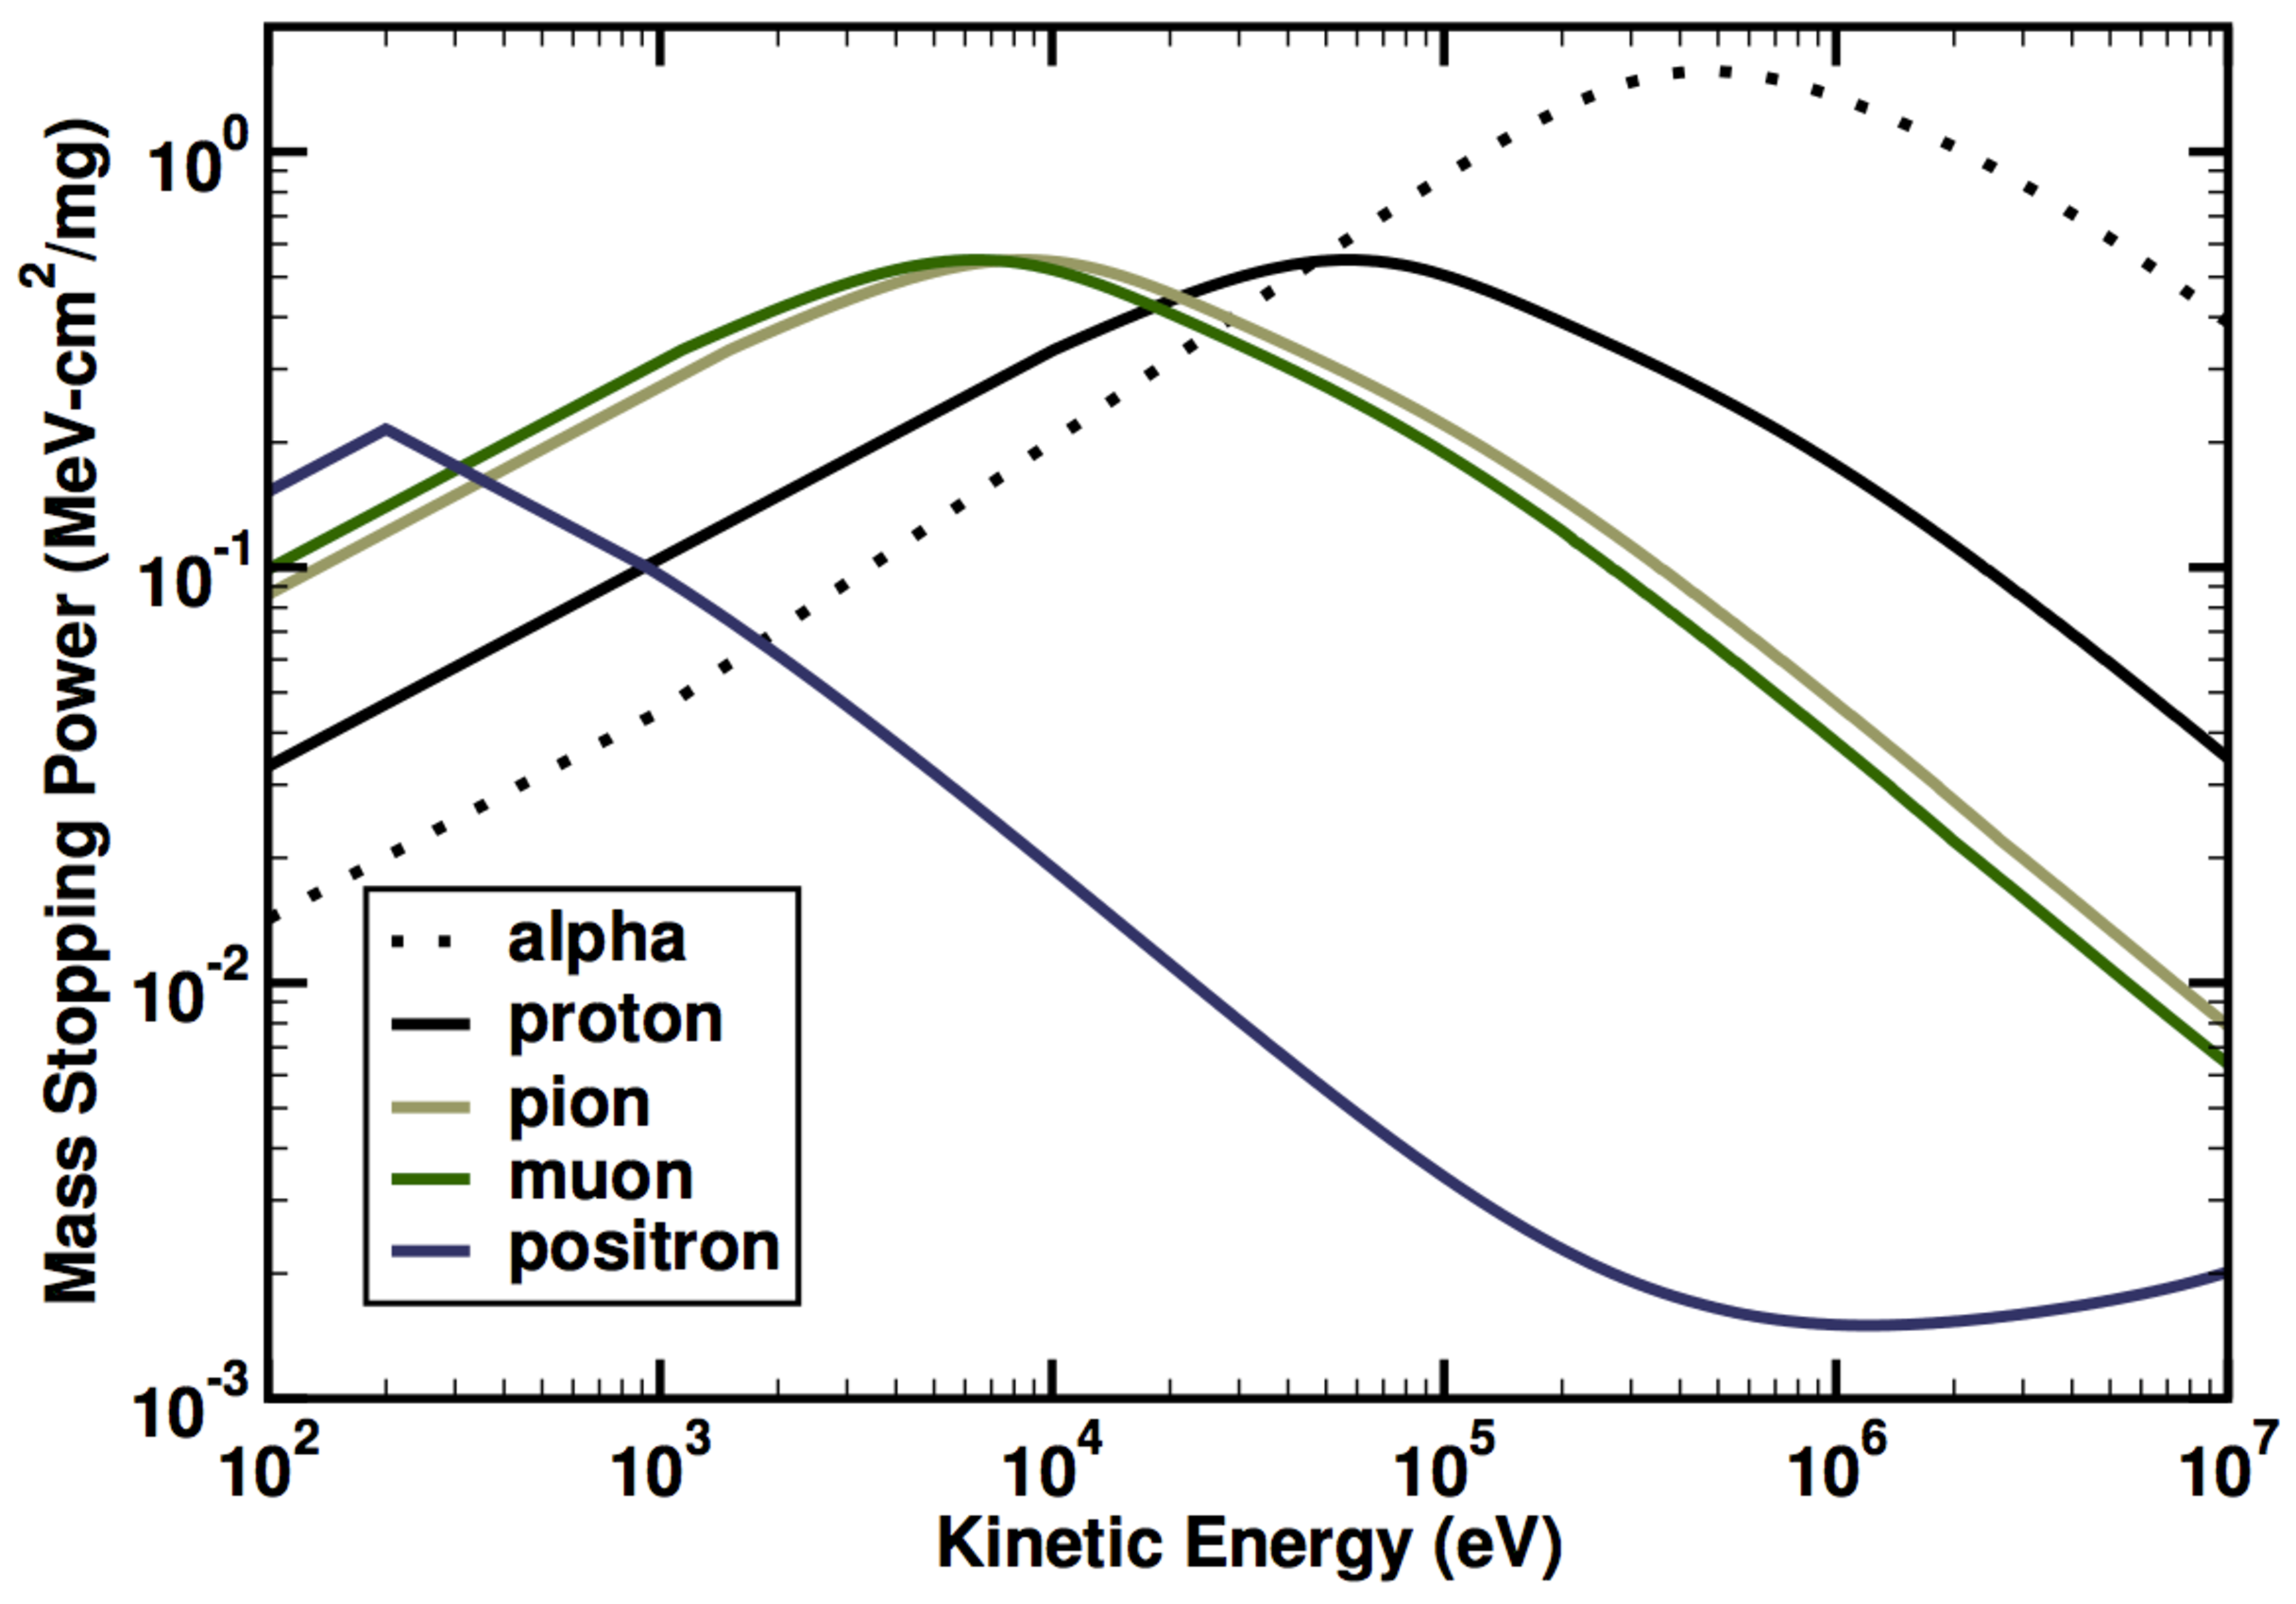
\includegraphics[width=4.5in]{stopping_power_proton_muon_sier_diss.pdf}
    \end{center}
    \caption[Mass stopping power extracted from Geant4 for protons, pions, muons, and positrons in silicon. Alpha particle stopping power shown for reference.]{Mass stopping power extracted from Geant4 for protons, pions, muons, and positrons in silicon. Alpha particle stopping power shown for reference \cite{Sierawski:2011bn}.}
    \label{fig:stopping_power_protons_muons}
\end{figure}

Like protons, muons are singly charged particles with a mass roughly 200 times that of the electron mass.
Fig.~\ref{fig:stopping_power_protons_muons} shows the stopping power, or mass stopping power, the rate of energy loss per unit path length, for a variety of particle species.
The curves for protons and muons are similar having a comparable magnitude.
The difference in the stopping power curves is due to the lower mass of the muon when compared to that of protons.
This parallel indicates that the energy deposition from stopping muons would be comparable to that of low-energy protons.
By induction, muons could therefore contribute to the soft error rate, particularly in the terrestrial environment, of SRAMs that exhibit sensitivity to low-energy protons.

Sierawski \emph{et al.} demonstrated that stopping muons were indeed capable of upsetting SRAMs fabricated in the 65~nm technology under reduced bias conditions \cite{Sierawski:2010cj}.
\begin{figure}[htbp]
    \begin{center}
        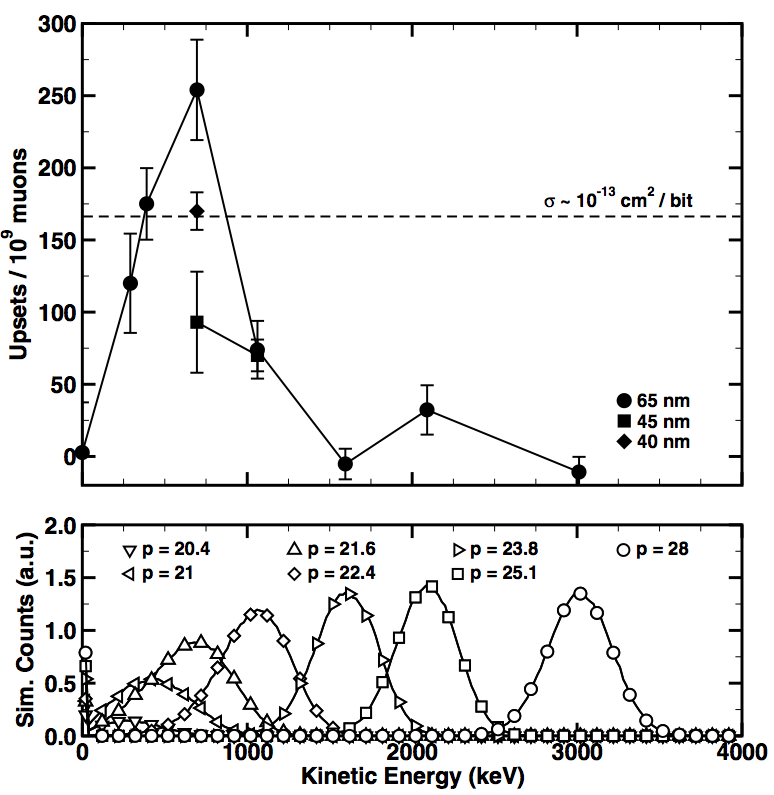
\includegraphics[width=4.5in]{muon_upsets_tech_generation.png}
    \end{center}
    \caption[Simulated muon kinetic energy distributions, as seen at the front of the part, corresponding to experimental momenta including upstream energy losses and straggling (bottom). Error counts for 65 nm, 45 nm, and 40 nm SRAMs versus estimated muon kinetic energy at 1.0 V bias (top). Dashed horizontal line represents an approximate muon-induced SEU cross section for reference.]{Simulated muon kinetic energy distributions, as seen at the front of the part, corresponding to experimental momenta including upstream energy losses and straggling (bottom). Error counts for 65 nm, 45 nm, and 40 nm SRAMs versus estimated muon kinetic energy at 1.0 V bias (top). Dashed horizontal line represents an approximate muon-induced SEU cross section for reference \cite{Sierawski:2010cj}.}
    \label{fig:muon_upsets_energy_dep}
\end{figure}
Fig.~\ref{fig:muon_upsets_energy_dep} plots the muon-induced upset cross-section as a function of incident muon energy.
The characteristics of Fig.~\ref{fig:muon_upsets_energy_dep} are quite similar to low-energy proton SEU cross-sections.
There is a flat region corresponding to the most energetic muons and as the incident muon energy is reduced there is an abrupt increase in the SEU cross-section.
Further reductions in incident muon energy result in particles with insufficient range to reach the sensitive region of the SRAM.
Consequently, the lowest energy muons do not contribute to the upset cross-section.

Fig.~\ref{fig:muon_upsets_bias_dep} shows the SEU response of a 65~nm SRAM as a function of supply voltage for incident muons with average energy of approximately 400~keV. 
For a nominal supply voltage of 1.2~V, few errors are observed. 
As the applied bias is reduced, there is a corresponding increase in the number of muon-induced upsets. 
As discussed regarding Eq.~\ref{eq:qcrit} and the bias dependence of low-energy protons in Section~\ref{sub:low_energy_proton_induced_seus}, reduction in supply voltage results in a corresponding reduction in critical charge.
Consequently, reduction in critical charge with decreasing supply voltage makes the SRAM test chip vulnerable to a wider range of incident muon energies, which explains the bias dependence shown in Fig.~\ref{fig:muon_upsets_bias_dep}.
\begin{figure}[htbp]
    \begin{center}
        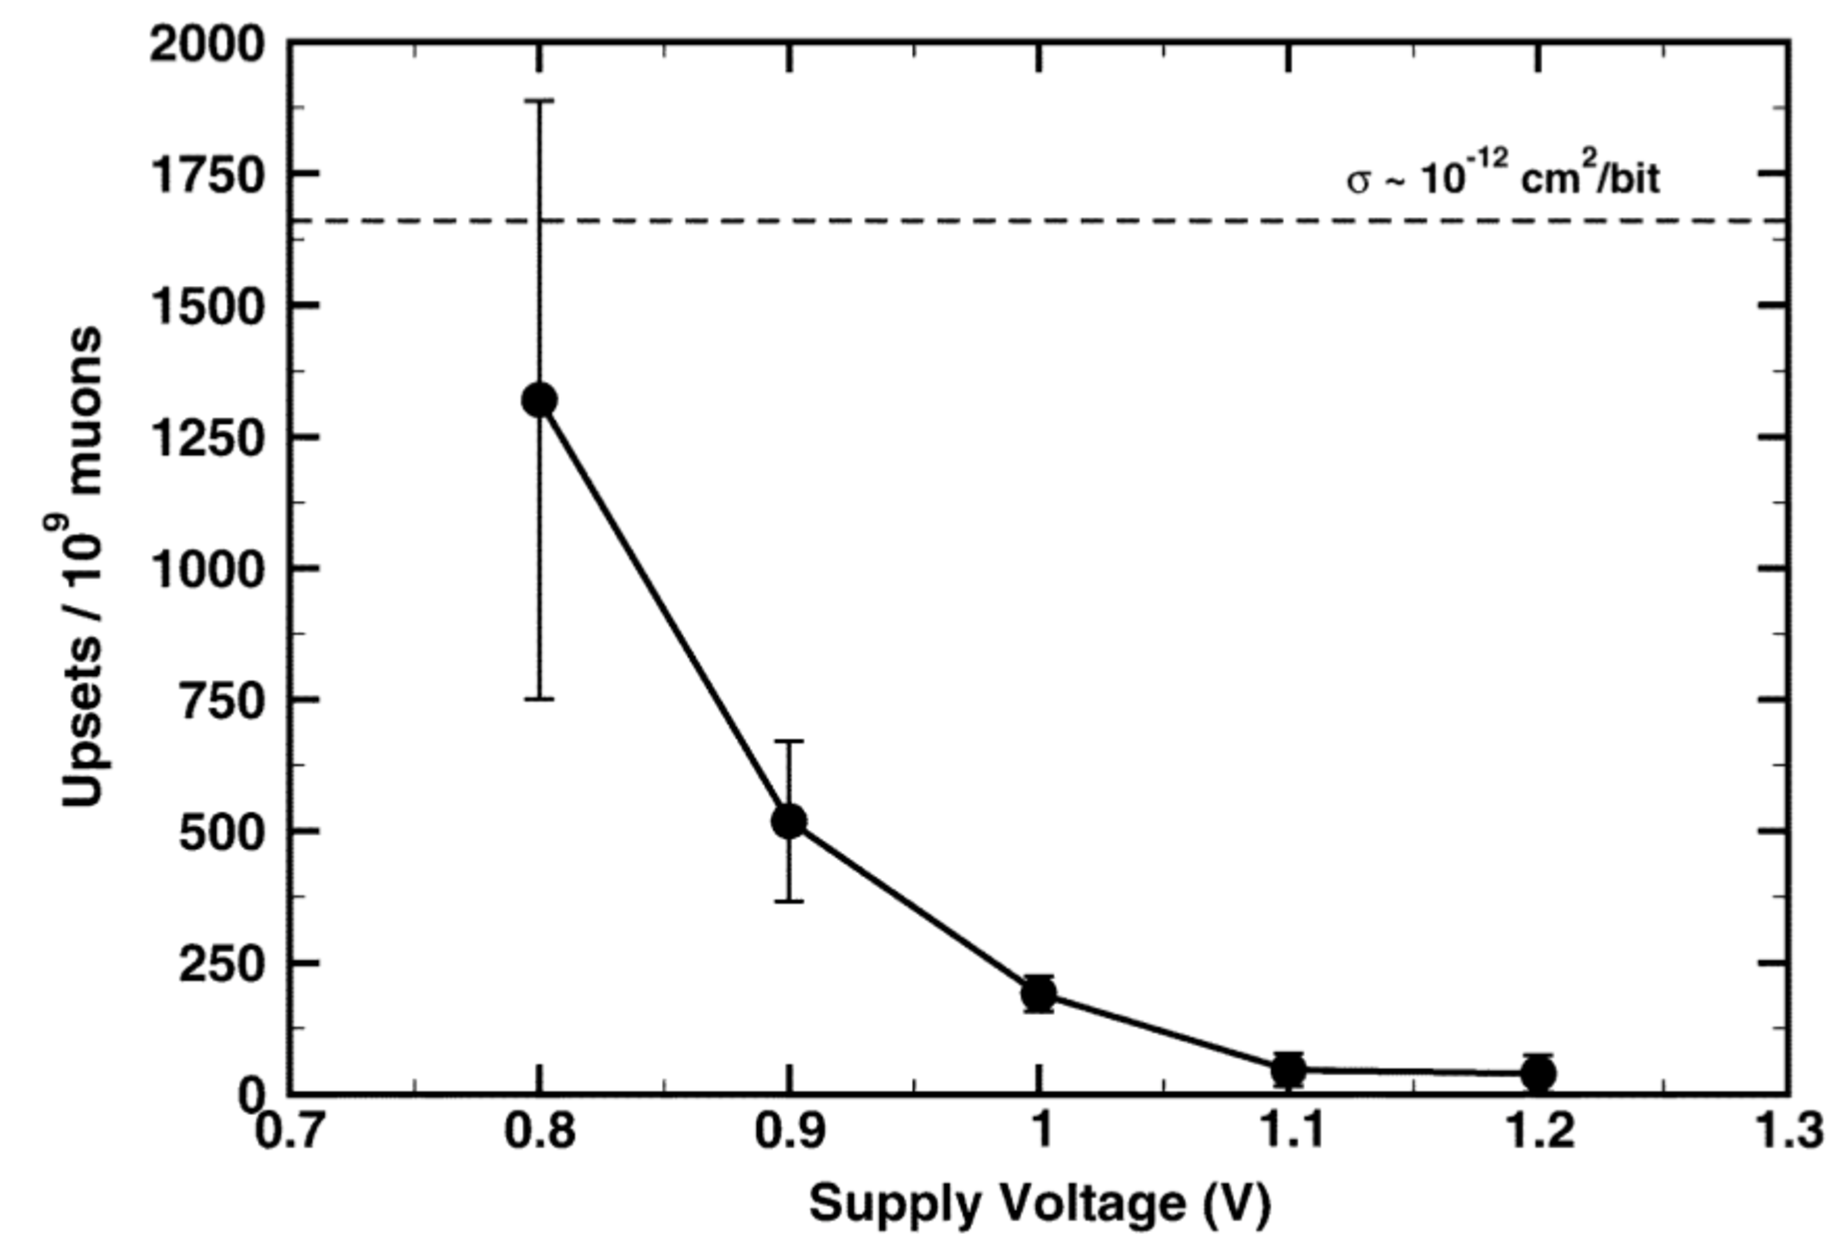
\includegraphics[width=4.5in]{muon_upsets_vdd_dep.pdf}
    \end{center}
    \caption[Error counts for 65~nm SRAM versus supply voltage for approximately 400~keV muons produced by 21~MeV/c momentum selection. Dashed horizontal line represents an approximate muon-induced SEU cross section for reference.]{Error counts for 65~nm SRAM versus supply voltage for approximately 400~keV muons produced by 21~MeV/c momentum selection. Dashed horizontal line represents an approximate muon-induced SEU cross section for reference \cite{Sierawski:2010cj}.}
    \label{fig:muon_upsets_bias_dep}
\end{figure}

The impact of muon-induced SEUs parallels that of effects due to low-energy protons.
The contribution of each has traditionally been considered negligible to the overall SEU cross-section and/or SER of modern SRAMs and has only recently been observed to contribute to error rates.
Ultimately, the observation of upsets due to low-energy protons and muons signal that commercial SRAM components are becoming increasingly sensitive to effects from a wider range of ionizing particle species.
The main goal of this dissertation is to expand on the observation of upsets due to lightly ionizing, singly-charged particles (low-energy protons and muons) and investigate whether SRAMs fabricated in modern, sub-65~nm technology nodes exhibit SEU sensitive to ionization from energetic electrons.
% subsection muon_induced_seus (end)


\subsection{SRAM Cell Imprinting} % (fold)
\label{sub:sram_cell_imprinting}
CMOS devices exposed to ionizing radiation can experience threshold voltage shifts and decreased carrier mobility as a result of accumulated dose in oxides and the formation of interface traps \cite{Dressendorfer:1981kg, Galloway:1990kh, Fleetwood:1993vs, Fleetwood:1995tk}. 
The severity of radiation induced degradation in devices is a complicated interaction dependent on the bias conditions during and after exposure. 
Because the drive strength of \emph{n}-channel MOSFETs is much higher than \emph{p}-channel devices, the total-ionizing dose (TID) response of CMOS SRAMs depends strongly on parametric shifts in the \emph{n}MOSFET device elements \cite{Schott:1987cx,Fleetwood:1987cfa}. 
While process hardening efforts may improve the circuits tolerance to TID, designs may still experience functional failure due to speed and timing degradation \cite{Fleetwood:1987cfa,Felix:2006jl}.

Radiation induced threshold voltage shifts in the \emph{n}MOSFET elements of CMOS SRAMs were initially reported to cause an imbalance in device turn-on voltages \cite{Arimura:1985wl}.
The data state of an SRAM establishes bias conditions for the transistor elements of the cross-coupled inverter when exposed to a source of ionizing radiation. 
The resulting cell imbalance of \emph{n}MOSFET threshold voltages causes in an asymmetry in switching voltage and SNM that is dependent on the stored data state of the cell. 
Fleetwood \emph{et al.} published a study seeking to quantify the ``worst-case'' SRAM radiation response by evaluating each possible bias condition. 
In \cite{Fleetwood:1987cfa}, the bias conditions are evaluated to a total dose of 1~Mrad(Si) and the results can be seen in Fig.~\ref{fig:sram_cell_imb_nmos_vth}.
During irradiation the initial threshold voltage shift, for both the ``on'' and ``off'' conditions, is negative, consistent with the build-up of charge in the gate oxide region \cite{Dressendorfer:1981kg,Galloway:1990kh}. 
For consistency, the \emph{1} state of the SRAM cell is defined to be when Q is low, that is when the transistor M3 of Fig.~\ref{fig:SRAM_Cell} is ``on''.
Fig.~\ref{fig:sram_cell_imb_nmos_vth} indicates that the devices irradiated in the ``off'' state experience a larger threshold voltage shift than those irradiated in the ``on'' state.
Additional exposure of the \emph{n}-channel devices shows a rebound effect, which is attributed to the accumulation of interface traps that very quickly begin to dominate the device response \cite{Fleetwood:1993vs,Galloway:1990kh}. 
Fig.~\ref{fig:sram_cell_imb_nmos_vth} shows that the accumulation of interface traps continues even after irradiation, resulting in large, positive threshold voltage shifts for each bias condition.

\begin{figure}[tb]
    \begin{center}
        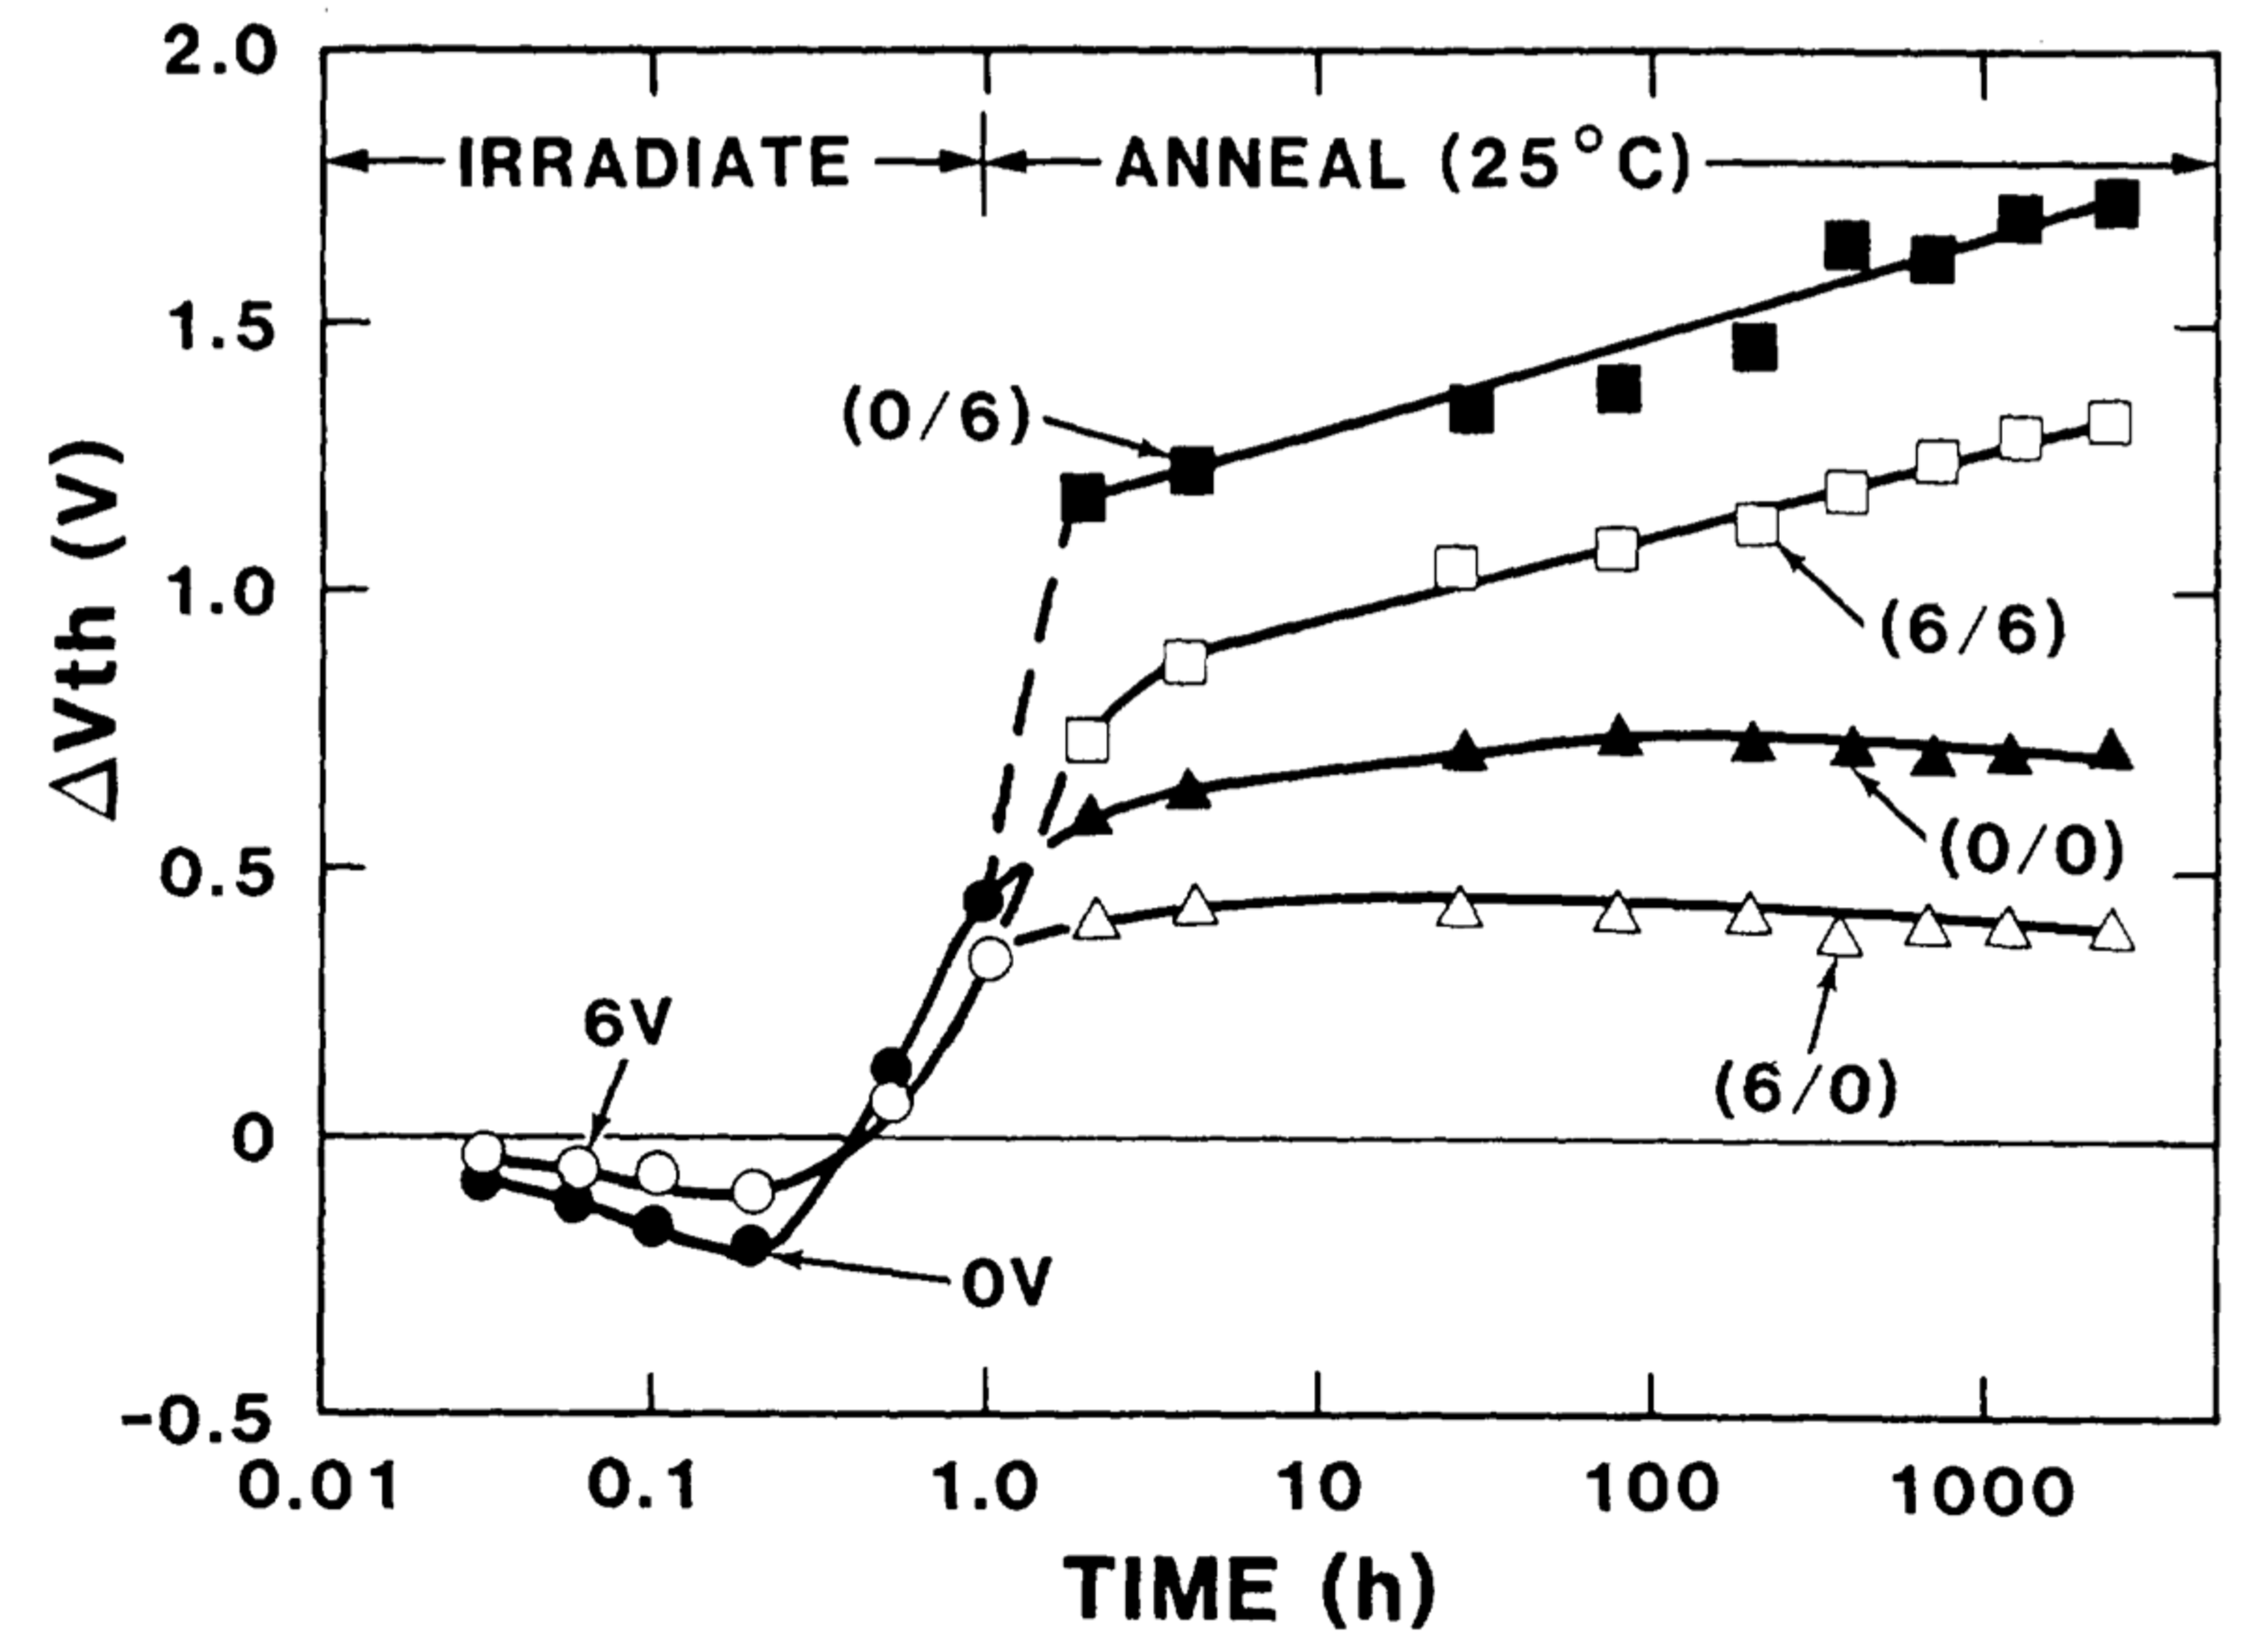
\includegraphics[width=5in]{fleetwood_nmos_irrad_imbalance.pdf}
    \end{center}
    \caption[$\Delta V_{th}$ versus time, for \emph{n}-channel transistors irradiated to 1.0 Mrad and annealed at 25$^\circ$C.]{$\Delta V_{th}$ versus time, for \emph{n}-channel transistors irradiated to 1.0 Mrad and annealed at 25$^\circ$C \cite{Fleetwood:1987cfa}.}
    \label{fig:sram_cell_imb_nmos_vth}
\end{figure}

The threshold voltage imbalance, $V_{imb}$, induced by bias conditions during irradiation can be quantified as
\begin{equation}
    \label{eq:vth_imb}
    V_{imb} = V_{TM1} - V_{TM3}
\end{equation}
where $V_{TM1}$ is the \emph{n}MOSFET transistor with the largest threshold voltage after irradiation and $V_{TM3}$ has the less positive threshold voltage.
As defined in Eq.~\ref{eq:vth_imb}, a positive value of $V_{imb}$ implies a preferred \emph{1} state for the SRAM cell.
Conversely, a negative value of $V_{imb}$ implies a preferred \emph{0} state for the cell.

\begin{figure}[tb]
    \begin{center}
        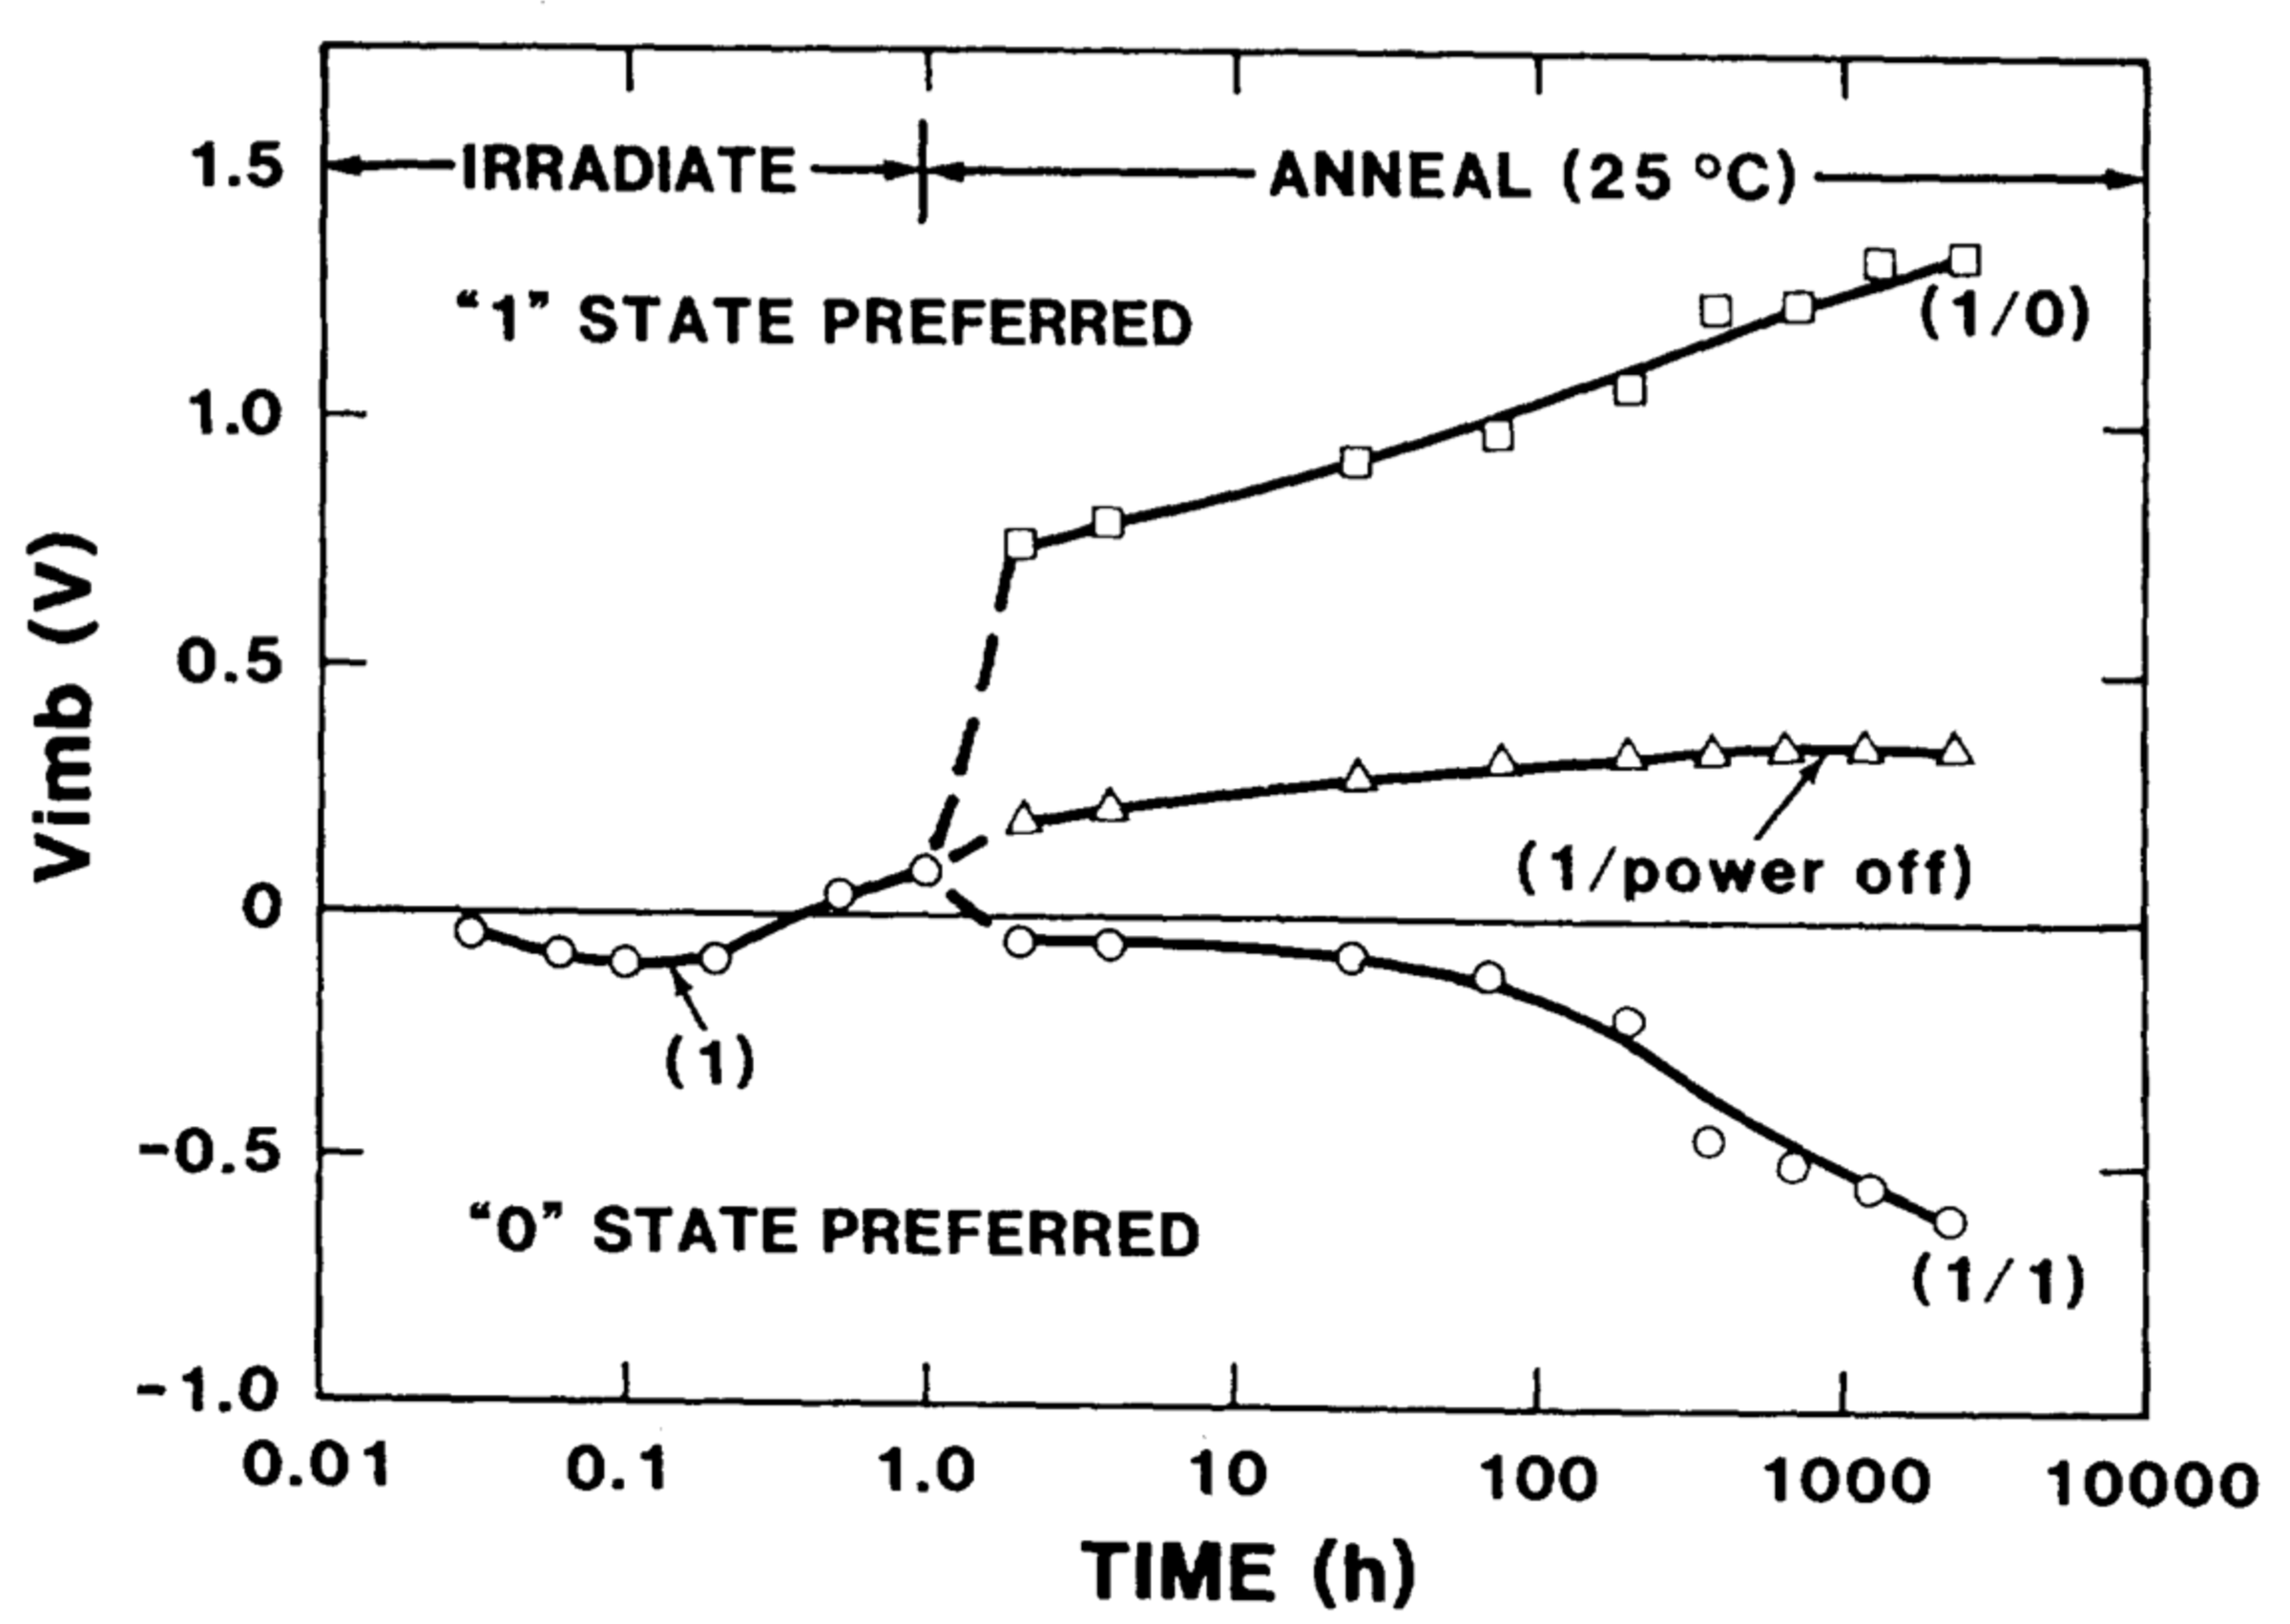
\includegraphics[width=5in]{fleetwood_nmos_irrad_imbalance_cases.pdf}
    \end{center}
    \caption{SRAM cell imbalance versus radiation and anneal time, based on the data of Fig.~\ref{fig:sram_cell_imb_nmos_vth}.}
    \label{fig:sram_cell_imb}
\end{figure}

A plot of threshold voltage imbalance versus irradiation and annealing time from \cite{Fleetwood:1987cfa} can be seen in Fig.~\ref{fig:sram_cell_imb} for conditions where the cell is initially in a \emph{1} state during irradiation and the cell state is either retained, rewritten, or power is removed from the cell during annealing.
Initial reports indicated that the SRAM cell was ``imprinted'' and the preferred state exclusively became that which it was irradiated under, however, Fig.~\ref{fig:sram_cell_imb} shows an initial preference for the \emph{0} state when the programmed pattern was the \emph{1} state. 
The preferred state of the SRAM therefore depends on bias conditions during irradiation and total dose accumulated \cite{Fleetwood:1987cfa}.
Cells irradiated in the \emph{1} state and annealed in the \emph{0} state show the strongest preference for the \emph{1} device state.
These bias conditions correspond to the largest positive threshold voltage shift in M1 and the least positive threshold voltage shift in M3, as shown in Fig.~\ref{fig:sram_cell_imb_nmos_vth}.
These conditions result in the largest speed and timing penalty, as well as the largest SRAM cell imbalance and are considered the ``worst-case'' conditions for TID in SRAMs.

\begin{figure}[tb]
    \begin{center}
        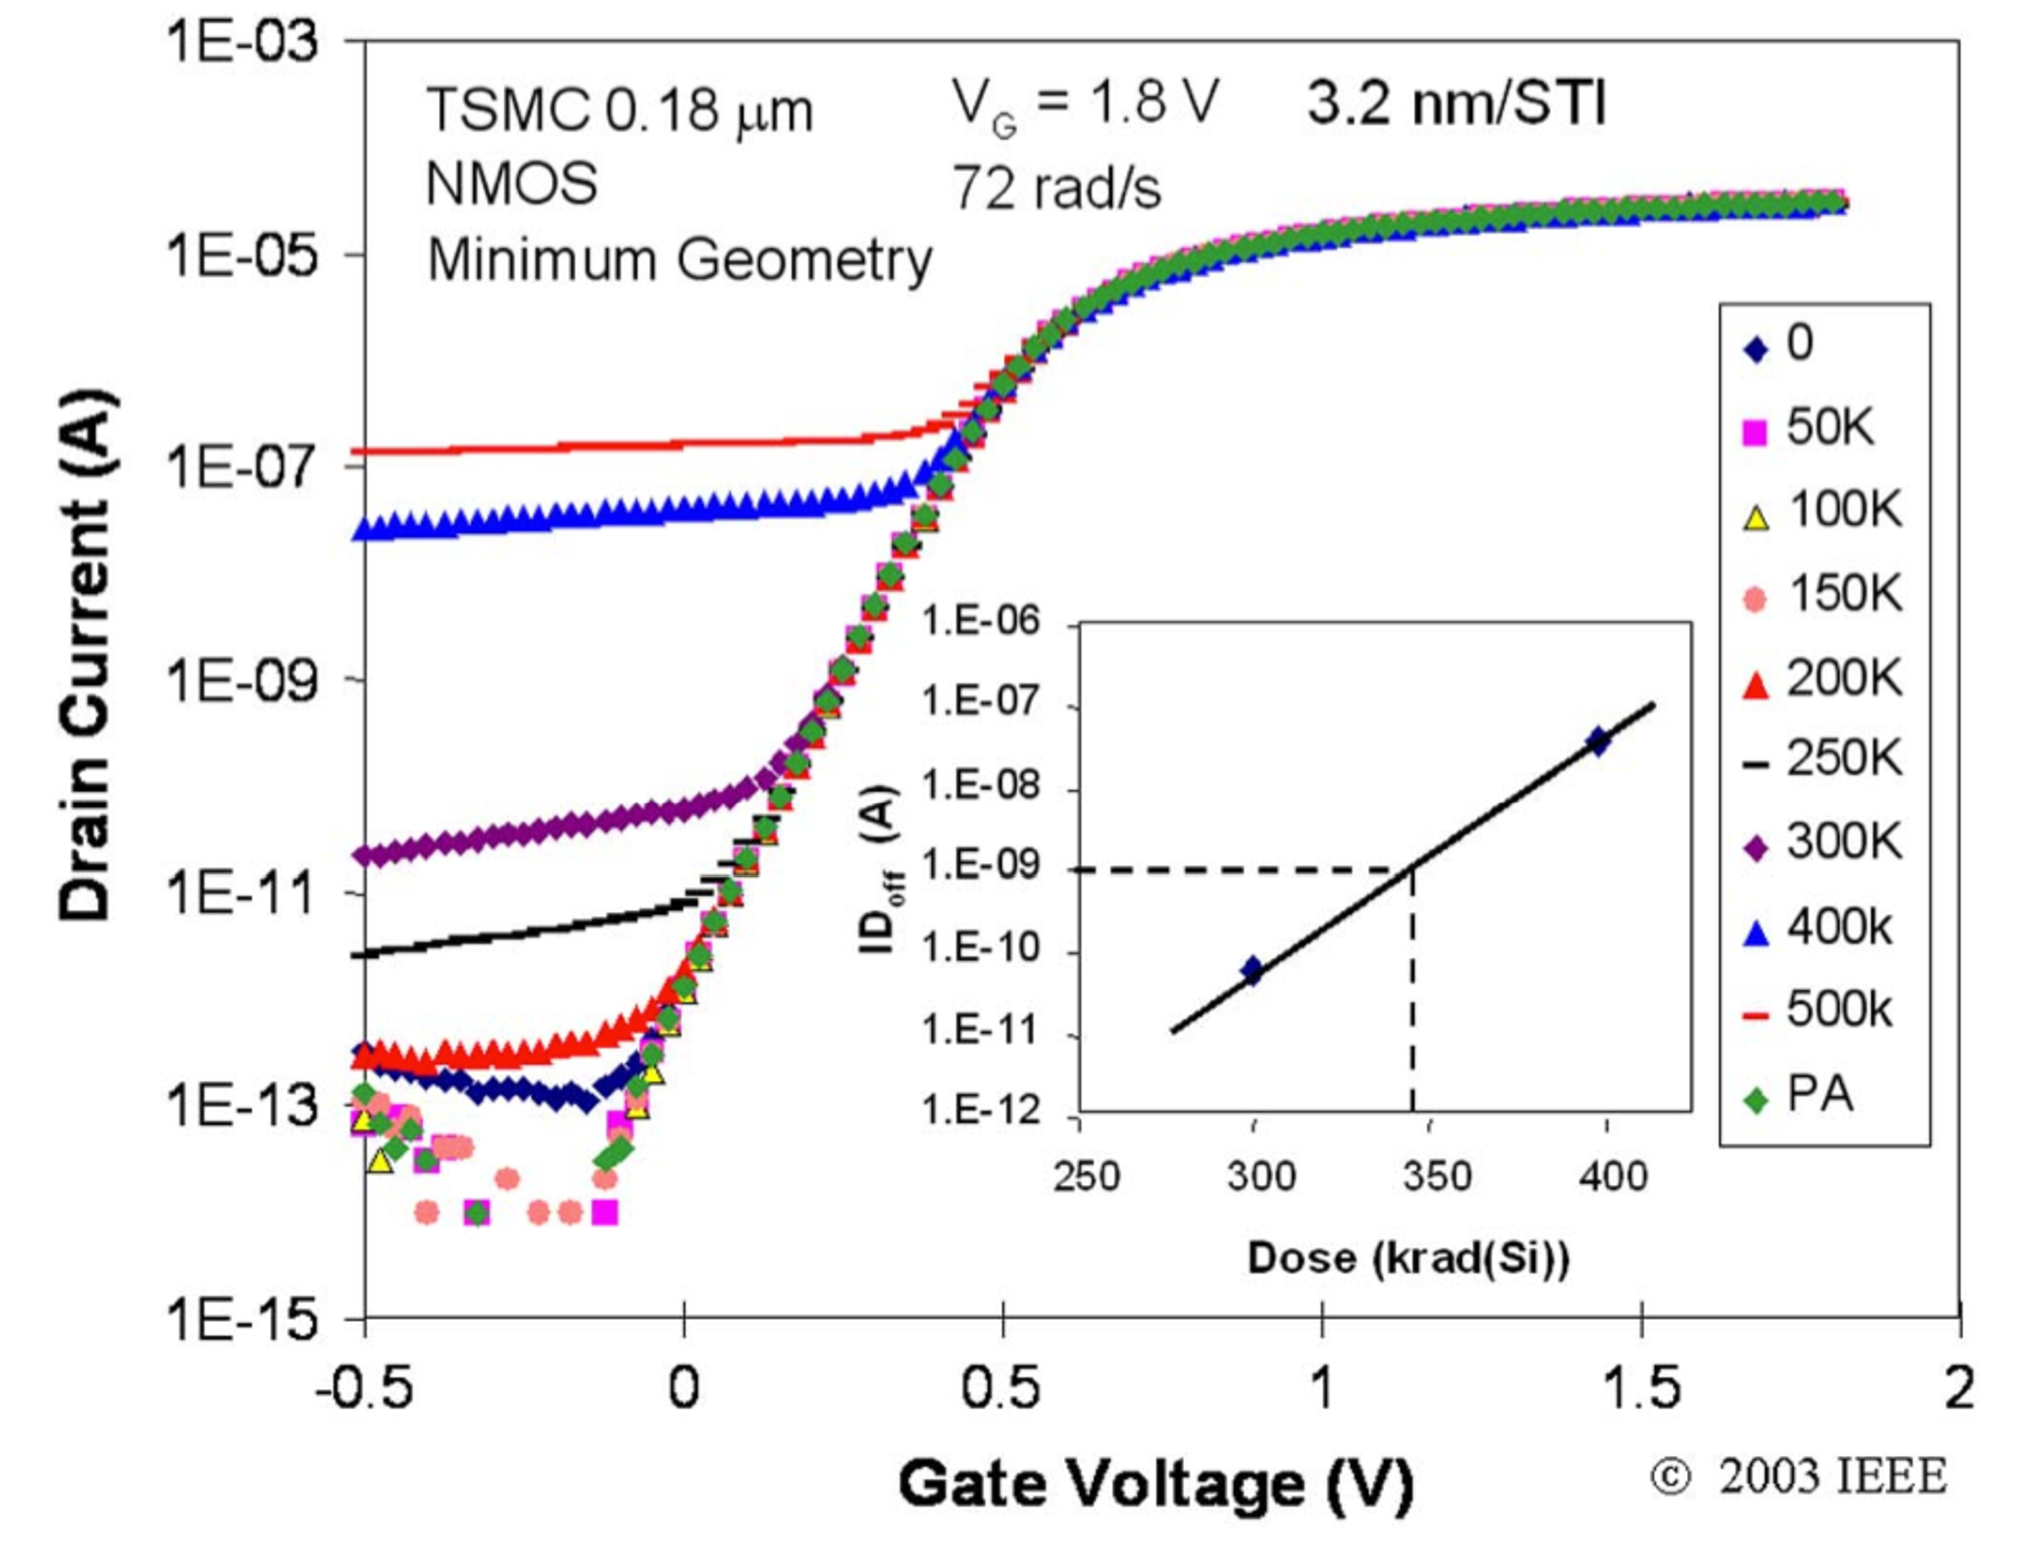
\includegraphics[width=4.5in]{barnaby_sti_leakage_tid.pdf}
    \end{center}
    \caption[Impact of STI radiation damage on the current-voltage characteristics of \emph{n}MOSFET fabricated in TSMC 0.18~$\mu$m CMOS.]{Impact of STI radiation damage on the current-voltage characteristics of \emph{n}MOSFET fabricated in TSMC 0.18~$\mu$m CMOS \cite{Barnaby:2006cp}}
    \label{fig:tid_sti_leak}
\end{figure}

The speed, timing degradation, and SRAM cell imbalances described above contribute to increased leakage current and functional failure of the SRAM cell.
Aggressive scaling of CMOS features size has resulted in a decrease in gate oxide thickness.
The magnitude of threshold voltage shifts observed in more modern technology nodes has reduced relative to nominal supply voltage. 
For a highly optimized process, even small changes in operating points can be a significant issue, in this case however, scaling has improved commercial CMOS tolerance to TID \cite{Barnaby:2006cp,Felix:2006jl}. 
Investigations by Felix and Yao have studied TID effects on more recent commercial CMOS SRAMs and conclude that below 90~nm SRAMs are highly resistant to ``pattern imprinting'' effects \cite{Felix:2006jl,Yao:2008ce,Nair:2013to}.
Along those lines, functional device failure at the 130~nm node did not typically occur until 200-400~krad(SiO$_2$) of dose accumulated within the device.
The failure mechanism was no longer reported to be threshold voltage shifts and mobility degradation, but increased sidewall leakage at the shallow trench isolation (STI)--silicon interface, an issue that has become increasingly problematic for current-generation technology nodes \cite{Felix:2006jl,Barnaby:2006cp}. 
Accumulation of charge in the STI activates a parasitic sidewall transistor along the edge of the device acting as a constant bias condition that may deplete or, given sufficient dose, invert nearby active silicon resulting in a static increase in leakage current.
The impact of charge build up in STI on transistor \emph{I-V} characteristics is shown in Fig.~\ref{fig:tid_sti_leak}.
It is important to note the lack of threshold voltage shift in Fig.~\ref{fig:tid_sti_leak}, instead a semi-static leakage increase is seen in the ``off'' region of the \emph{n}-channel device, effectively swamping the device response at sufficiently high dose and reducing the on/off current ratio by many orders of magnitude.
This is problematic for present-generation technology nodes because increased leakage currents can interfere with proper pre-charging and small signal development on bit-lines \cite{Yao:2008ce}.

\begin{figure}[tb]
    \begin{center}
        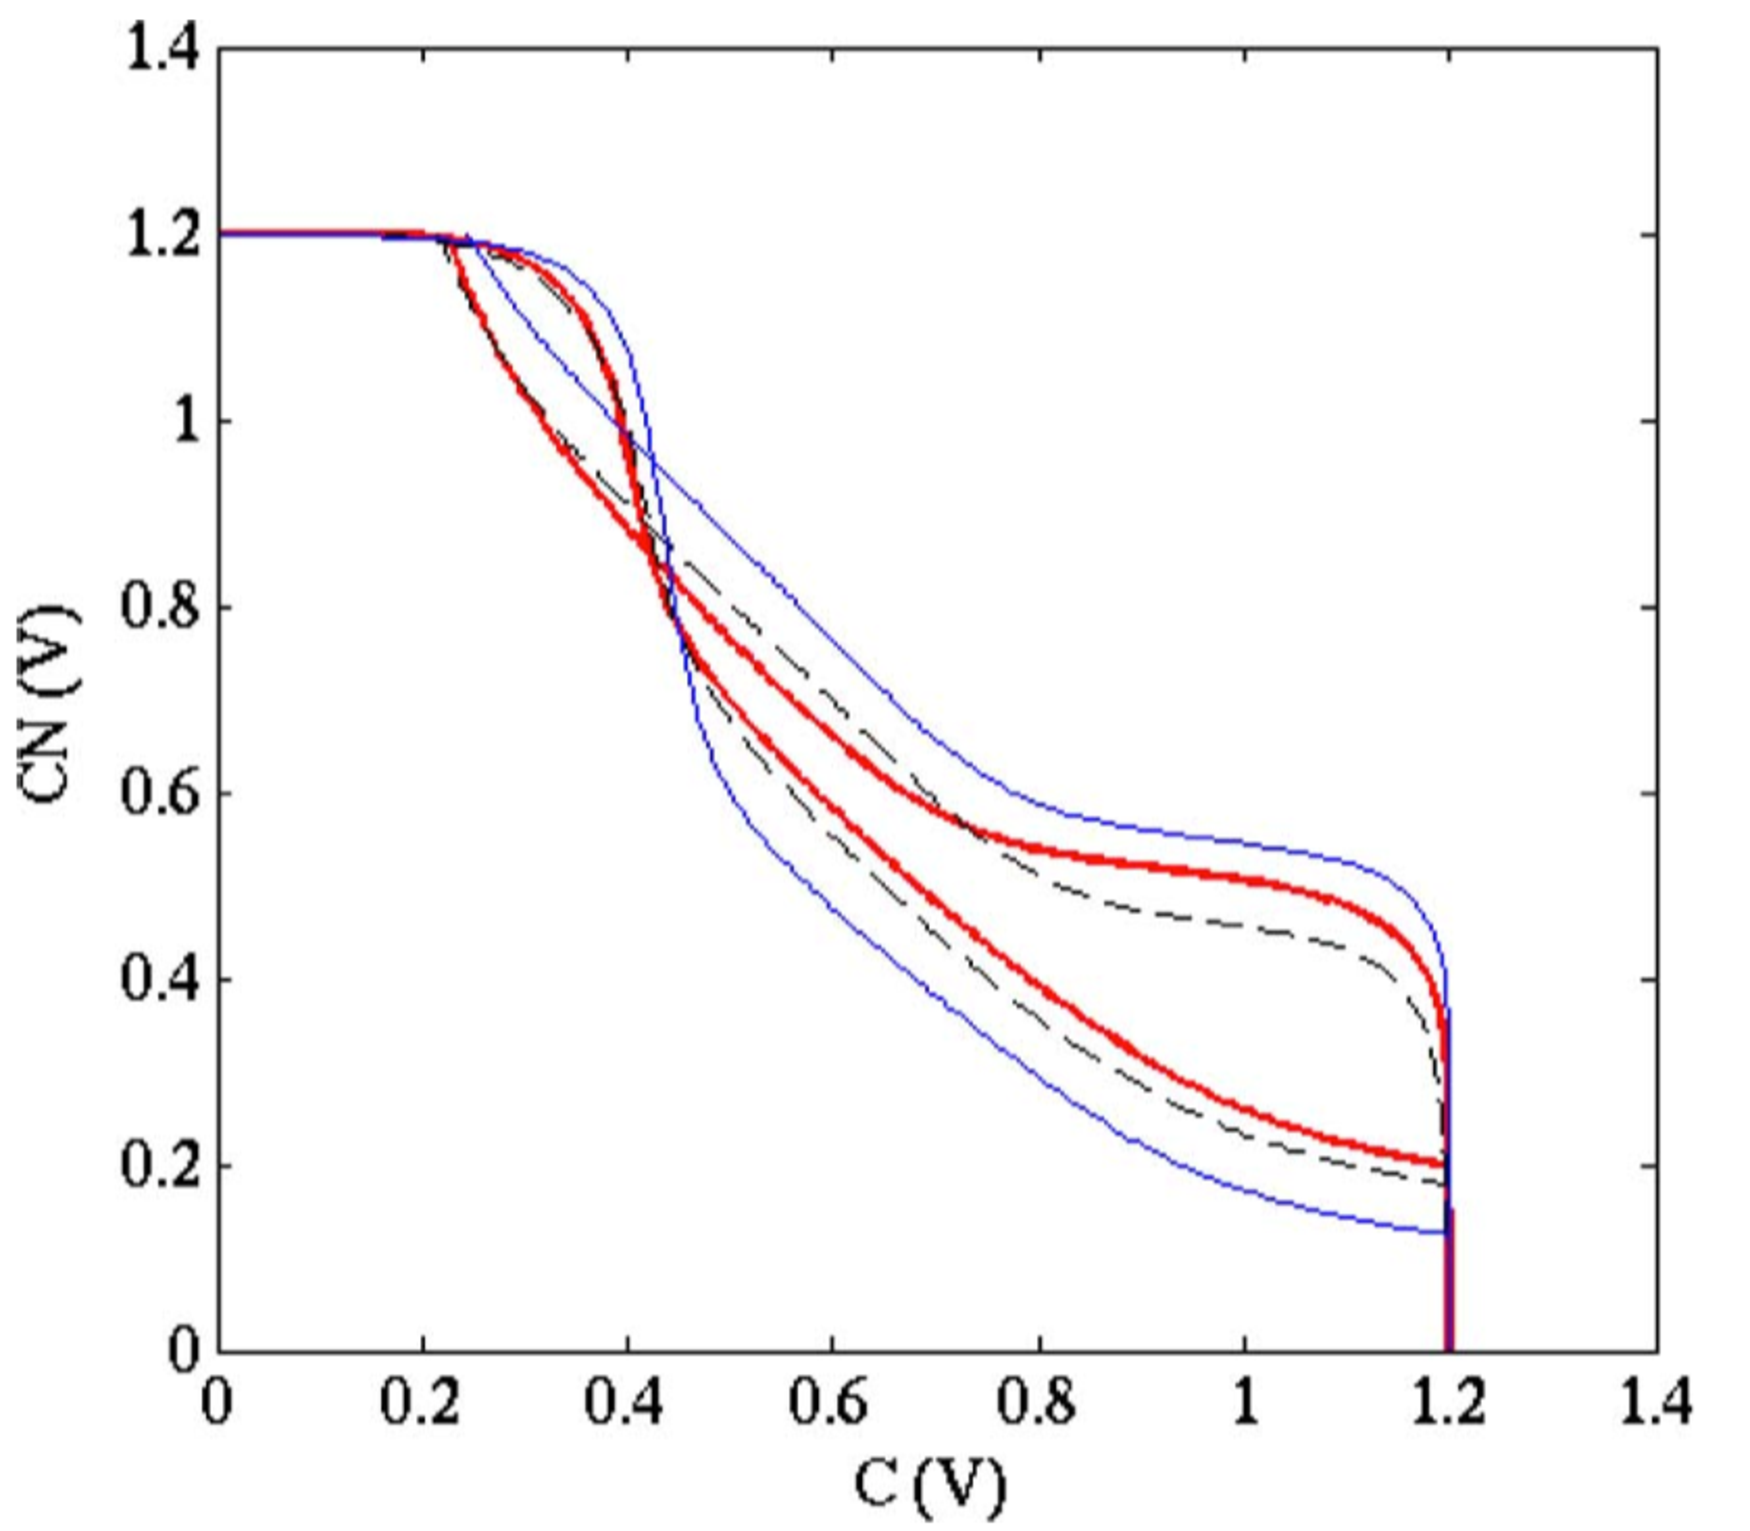
\includegraphics[width=5in]{snm_shift_postrad_yao_etal.pdf}
    \end{center}
    \caption[Worst-case Monte Carlo derived read SNM pre- and post-irradiation. The thin blue and dashed green lines show the post-irradiation SNM, while the thick red lines show the pre-irradiation response. The worst-case, i.e., the smallest box that fits within the ``eyes'' is improved after irradiation.]{Worst-case Monte Carlo derived read SNM pre- and post-irradiation. The thin blue and dashed green lines show the post-irradiation SNM, while the thick red lines show the pre-irradiation response. The worst-case, i.e., the smallest box that fits within the ``eyes'' is improved after irradiation \cite{Yao:2008ce}.}
    \label{fig:snm_shift_tid_yao}
\end{figure}

As a consequence of degraded speed, timing, threshold voltage imbalances, and increased leakage, irradiated SRAMs exhibit reduced SNMs and have been reported to have increased sensitivity to SEU from heavy-ion and transient irradiation \cite{Fleetwood:1987cfa,Bhuva:1987tq,Brucker:1986fb,Yao:2008ce,Felix:2006jl}.
In \cite{Yao:2008ce}, the 90~nm technology node did not exhibit a significant increase in supply current until approximately 300~krad(Si).
This is also the point at which ``imprinting'' began to become significant across the entire test chip.
Despite a dramatic increase in supply current, the devices were reported to remain completely functional while maintaining the programmed state to a total dose of 1~Mrad(Si).

\begin{figure}[htbp]
    \begin{center}
        \subfigure[]{
            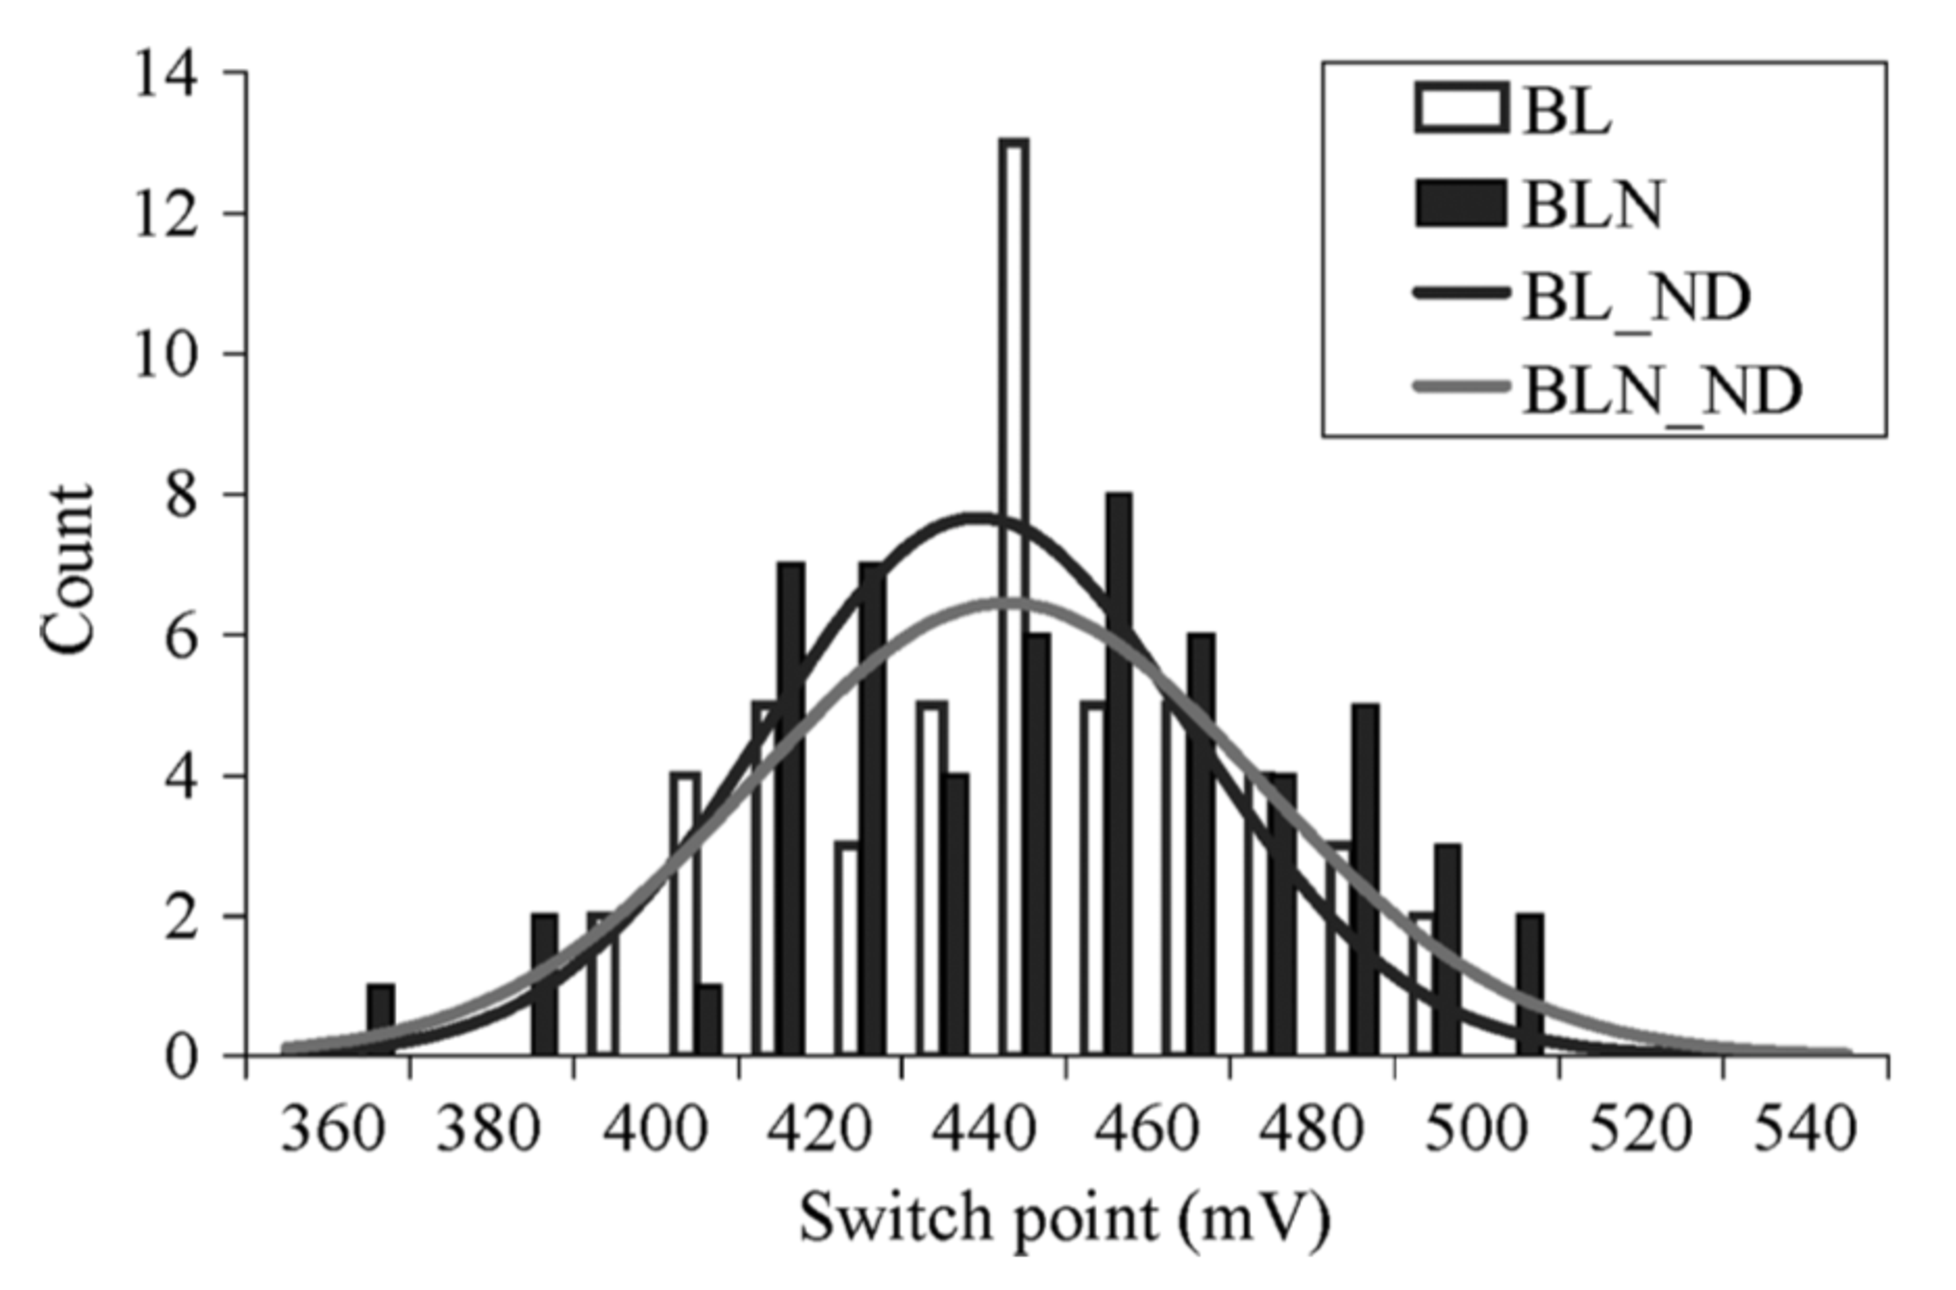
\includegraphics[width=4in]{sram_switch_pnt_yao_etal.pdf}
            \label{fig:prerad_swt_pnt_yao}
            }
        %\newline
        \subfigure[]{
            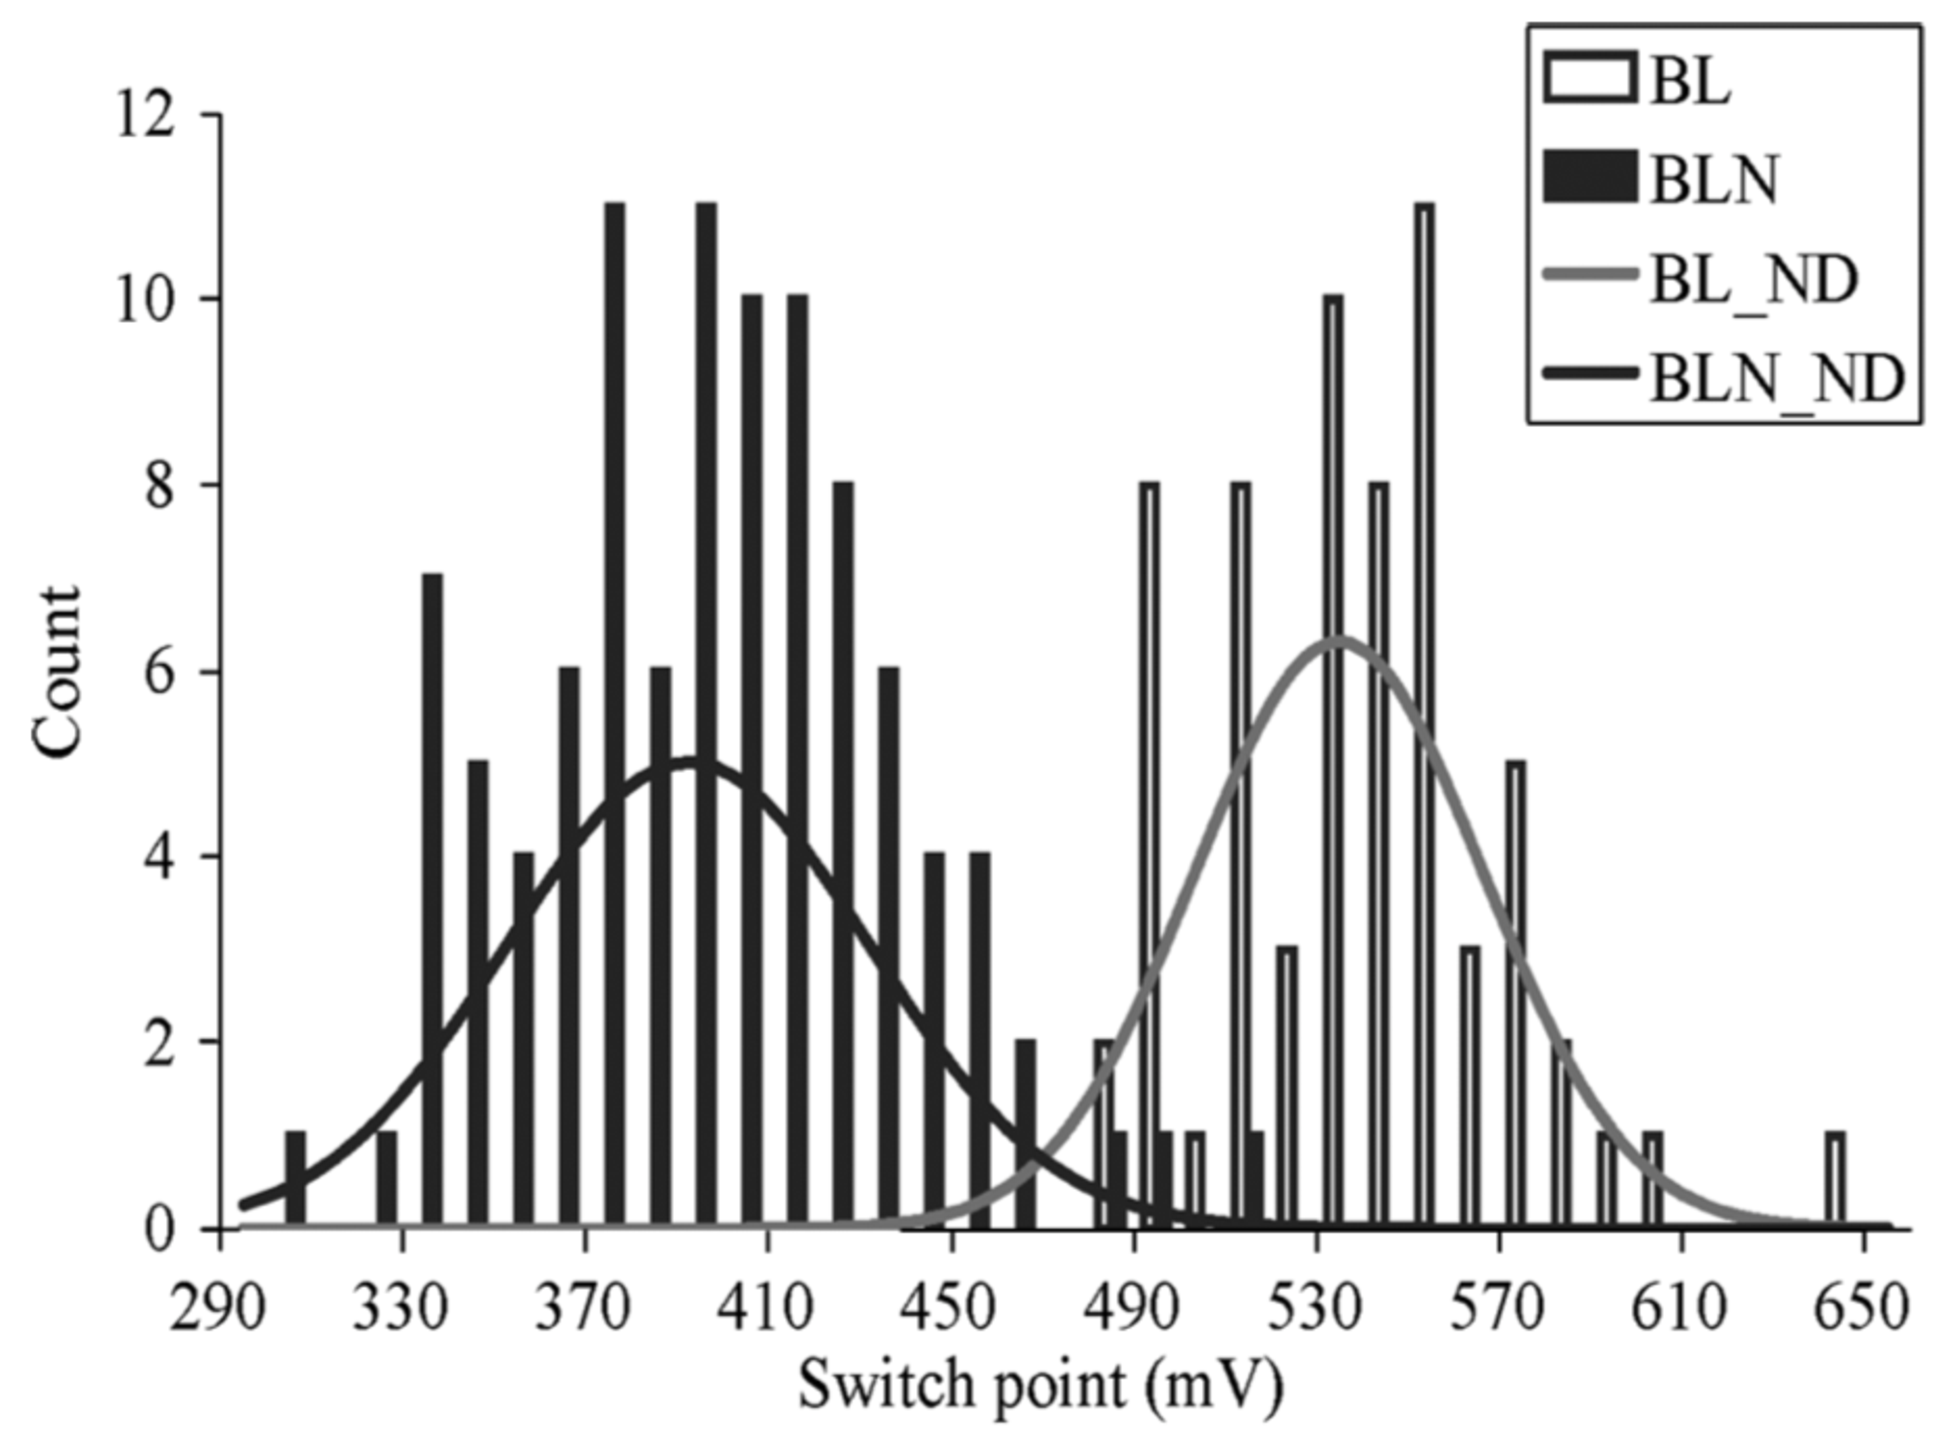
\includegraphics[width=4in]{sram_switch_pnt_postrad_yao_etal.pdf}
            \label{fig:postrad_swt_pnt_yao}
            }
    \end{center}
    \caption[Pre-irradiation SRAM cell trip points measured driving the $BL$ and $\overline{BL}$, shown in (a). $BL_{ND}$ and $\overline{BL}_{ND}$ are normal distribution curves for the SRAM DC switch point. In (b), measured SRAM cell node trip points after irradiation to 1.5 Mrad(Si). The $BL$ trip points are shifted up, i.e., the write margin is increased (easier write) and the $\overline{BL}$ write margin is reduced (it becomes more difficult to write).]{Pre-irradiation SRAM cell trip points measured driving the $BL$ and $\overline{BL}$, shown in (a). $BL_{ND}$ and $\overline{BL}_{ND}$ are normal distribution curves for the SRAM DC switch point. In (b), measured SRAM cell node trip points after irradiation to 1.5 Mrad(Si). The $BL$ trip points are shifted up, i.e., the write margin is increased (easier write) and the $\overline{BL}$ write margin is reduced (it becomes more difficult to write). After \cite{Yao:2008ce}.}
    \label{fig:sram_swt_pnts_yao}
\end{figure}

Yao \emph{et al.} used Monte Carlo simulations to infer the change in inverter transfer characteristics as a result of TID in a 90~nm technology node, which can be seen in Fig.~\ref{fig:snm_shift_tid_yao}.
The thin blue and dashed green lines show the post-irradiation SNM, while the thick red lines show the pre-irradiation response. The worst-case, i.e., the smallest box that fits within the ``eyes'' is improved after irradiation
The transfer characteristics shown in Fig.~\ref{fig:snm_shift_tid_yao} are drastically different from the symmetric response discussed previously regarding the 22~nm node and shown in Fig.~\ref{fig:22nm_soi_sram_butterfly_curve_snm}. 
Fig.~\ref{fig:sram_swt_pnts_yao} shows the pre- and post-irradiation SRAM cell switching points for the bit-line and bit-line complement.
The pre-irradiation data show a very symmetric, balanced cell response, indicating that neither cell state is preferred by the SRAM cell.
After exposure to 1.5~Mrad(Si) the characteristics shift forcing the cell into an asymmetric state where the $BL$ is easier to write than the $\overline{BL}$.
Within some margin this effectively constitutes functional SRAM cell failure, where it becomes nearly impossible, or at least exceedingly difficult, to read or write an SRAM cell and maintain valid data in the standby mode.

% subsection sram_cell_imprinting (end)

\subsection{Impact of Transient Radiation on SRAMs} % (fold)
\label{sub:railspan_collapse}
When semiconductor materials are exposed to high-intensity, penetrating radiation, such as X-rays or $\gamma$-rays, \emph{e-h} pairs are generated that may be collected and contribute to the cumulative photocurrent.
Photocurrents arise from high-flux irradiation conditions, such as those obtained from flash X-ray and pulsed reactor sources, and are ``global'' currents resulting from irradiation across an entire chip.
Because generated photocurrents are ``global'', every device on a common substrate will contribute to the collection of generated \emph{e-h} pairs during irradiation.

In 1964, Wirth and Rogers developed a mathematical model based on the continuity and diffusion equations that describes the transient currents generated as a result of high-intensity irradiation \cite{Wirth:1964kp}.
The model presented by Wirth and Rogers was refined and applied to the case of bipolar transistors by Long \emph{et al.} in \cite{Long:1983fg}, which accounted for differences in diffusion length and carrier lifetimes associated with an epitaxial layer on a highly doped substrate.
The conditions evaluated in \cite{Long:1983fg} are analogous to the case of  SRAM cell well junction photocurrents when exposed to a transient radiation environment.

Massengill \emph{et al.} applied the models and analysis presented in \cite{Long:1983fg} to the case of transient radiation upsets in CMOS SRAMs in \cite{Massengill:1984hn,Massengill:1985gd,Massengill:1986kp}. 
\begin{figure}[htbp]
    \begin{center}
        \subfigure[]{
            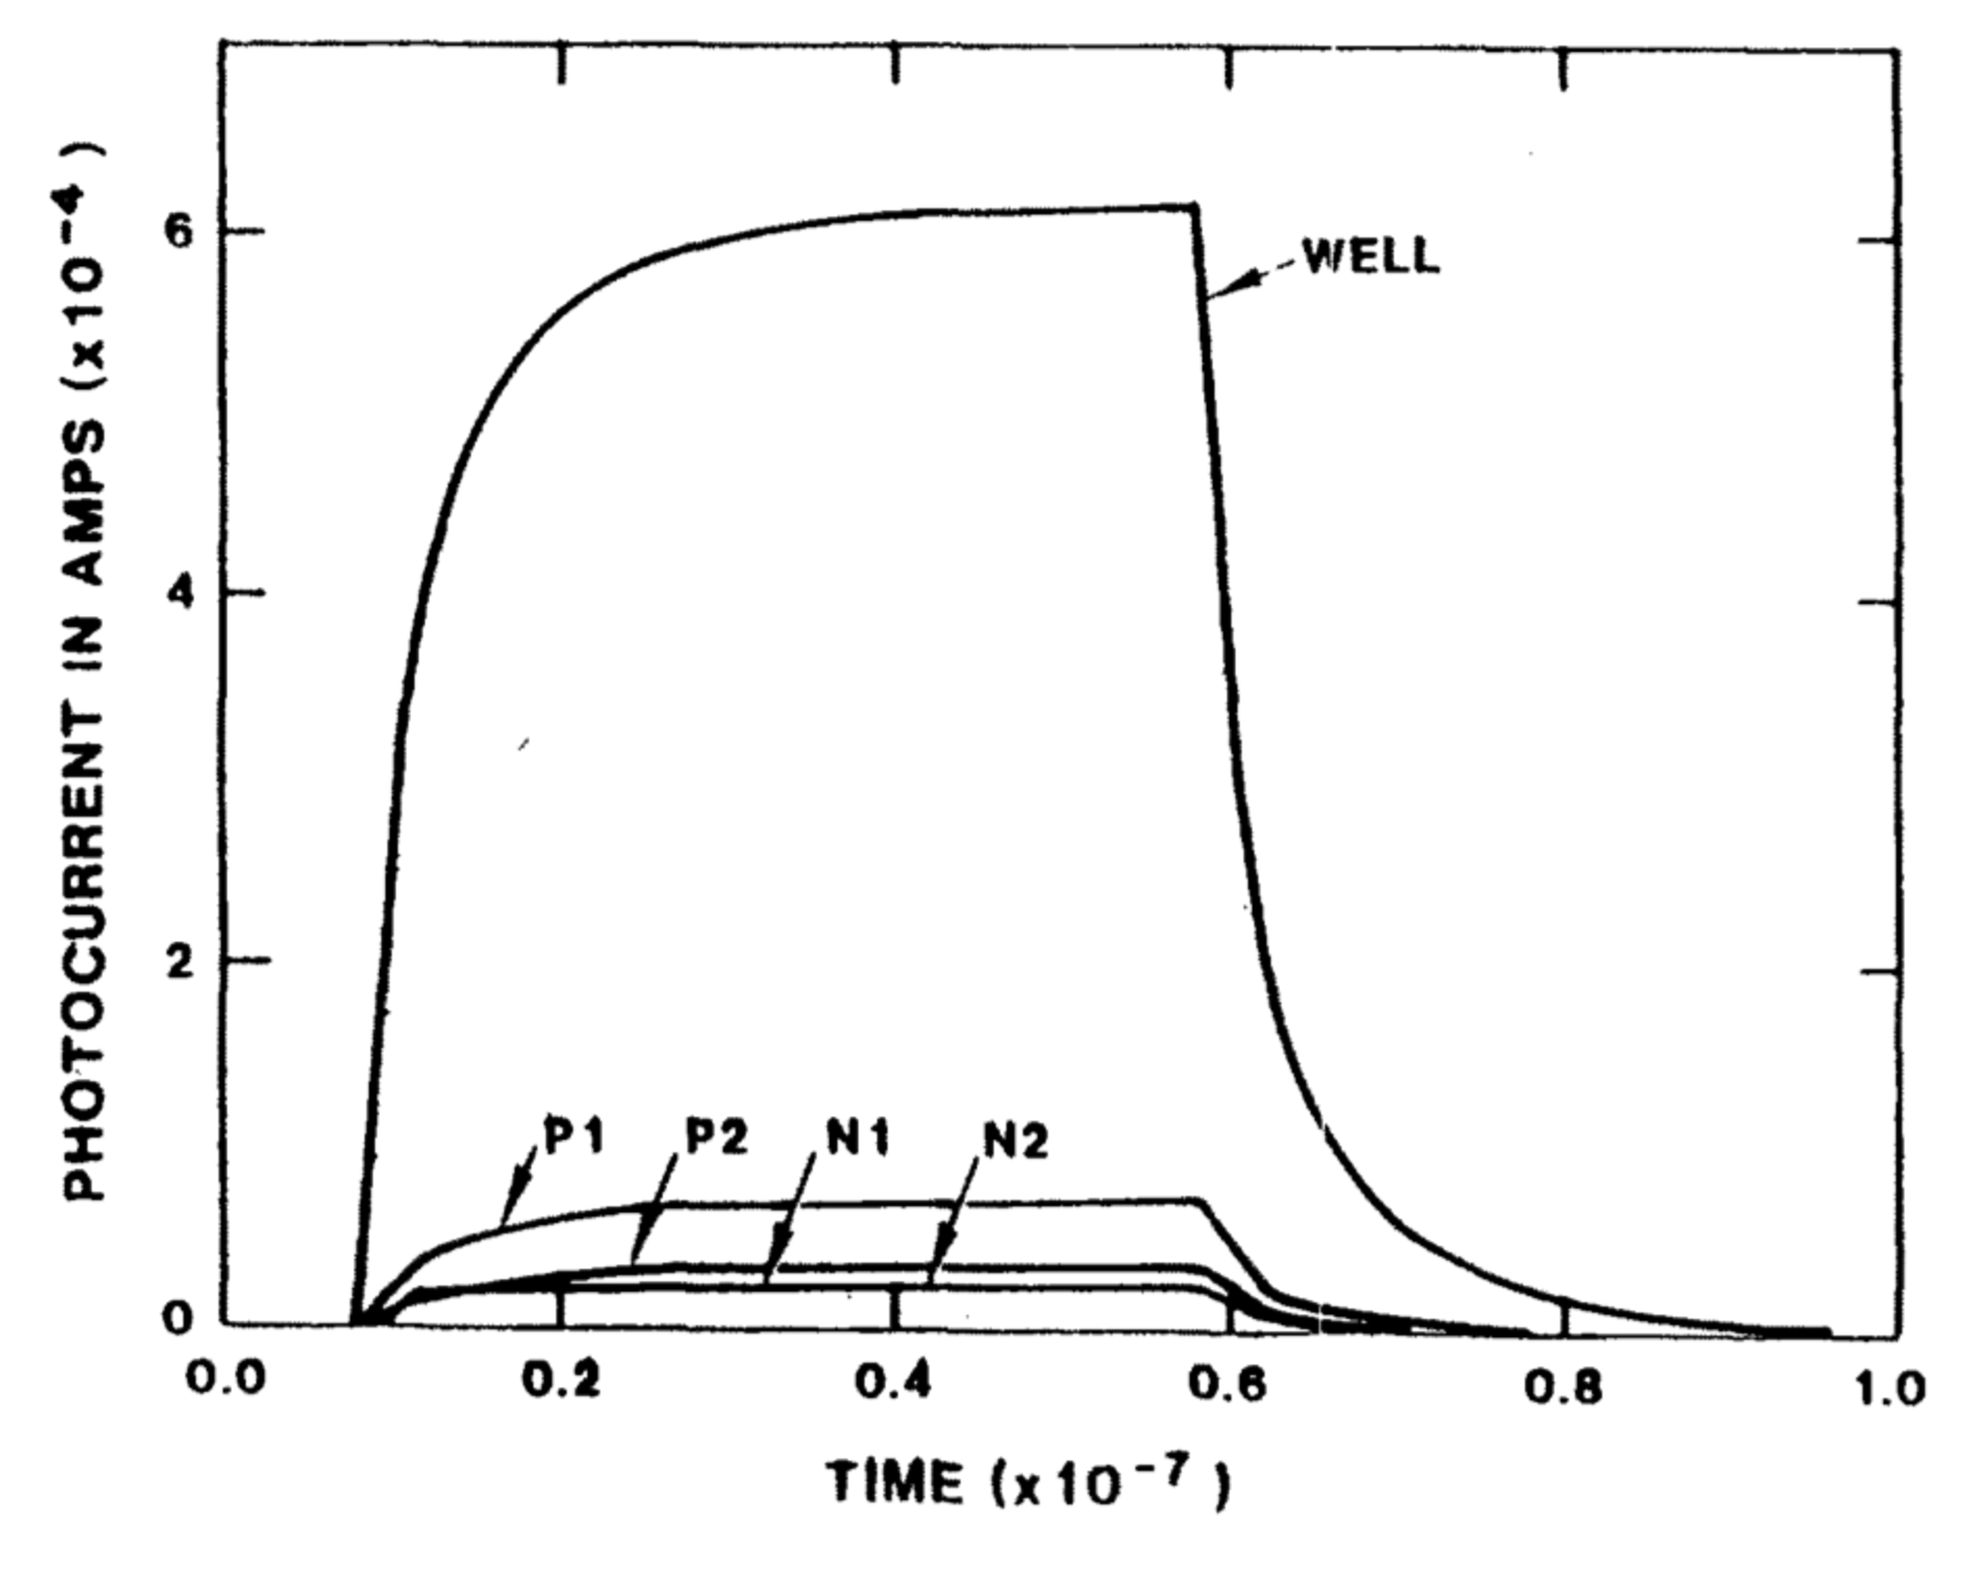
\includegraphics[width=4in]{photocurrents_local_well_bulk.pdf}
            \label{fig:photocurrents_sram_bulk}
            }
        \subfigure[]{
            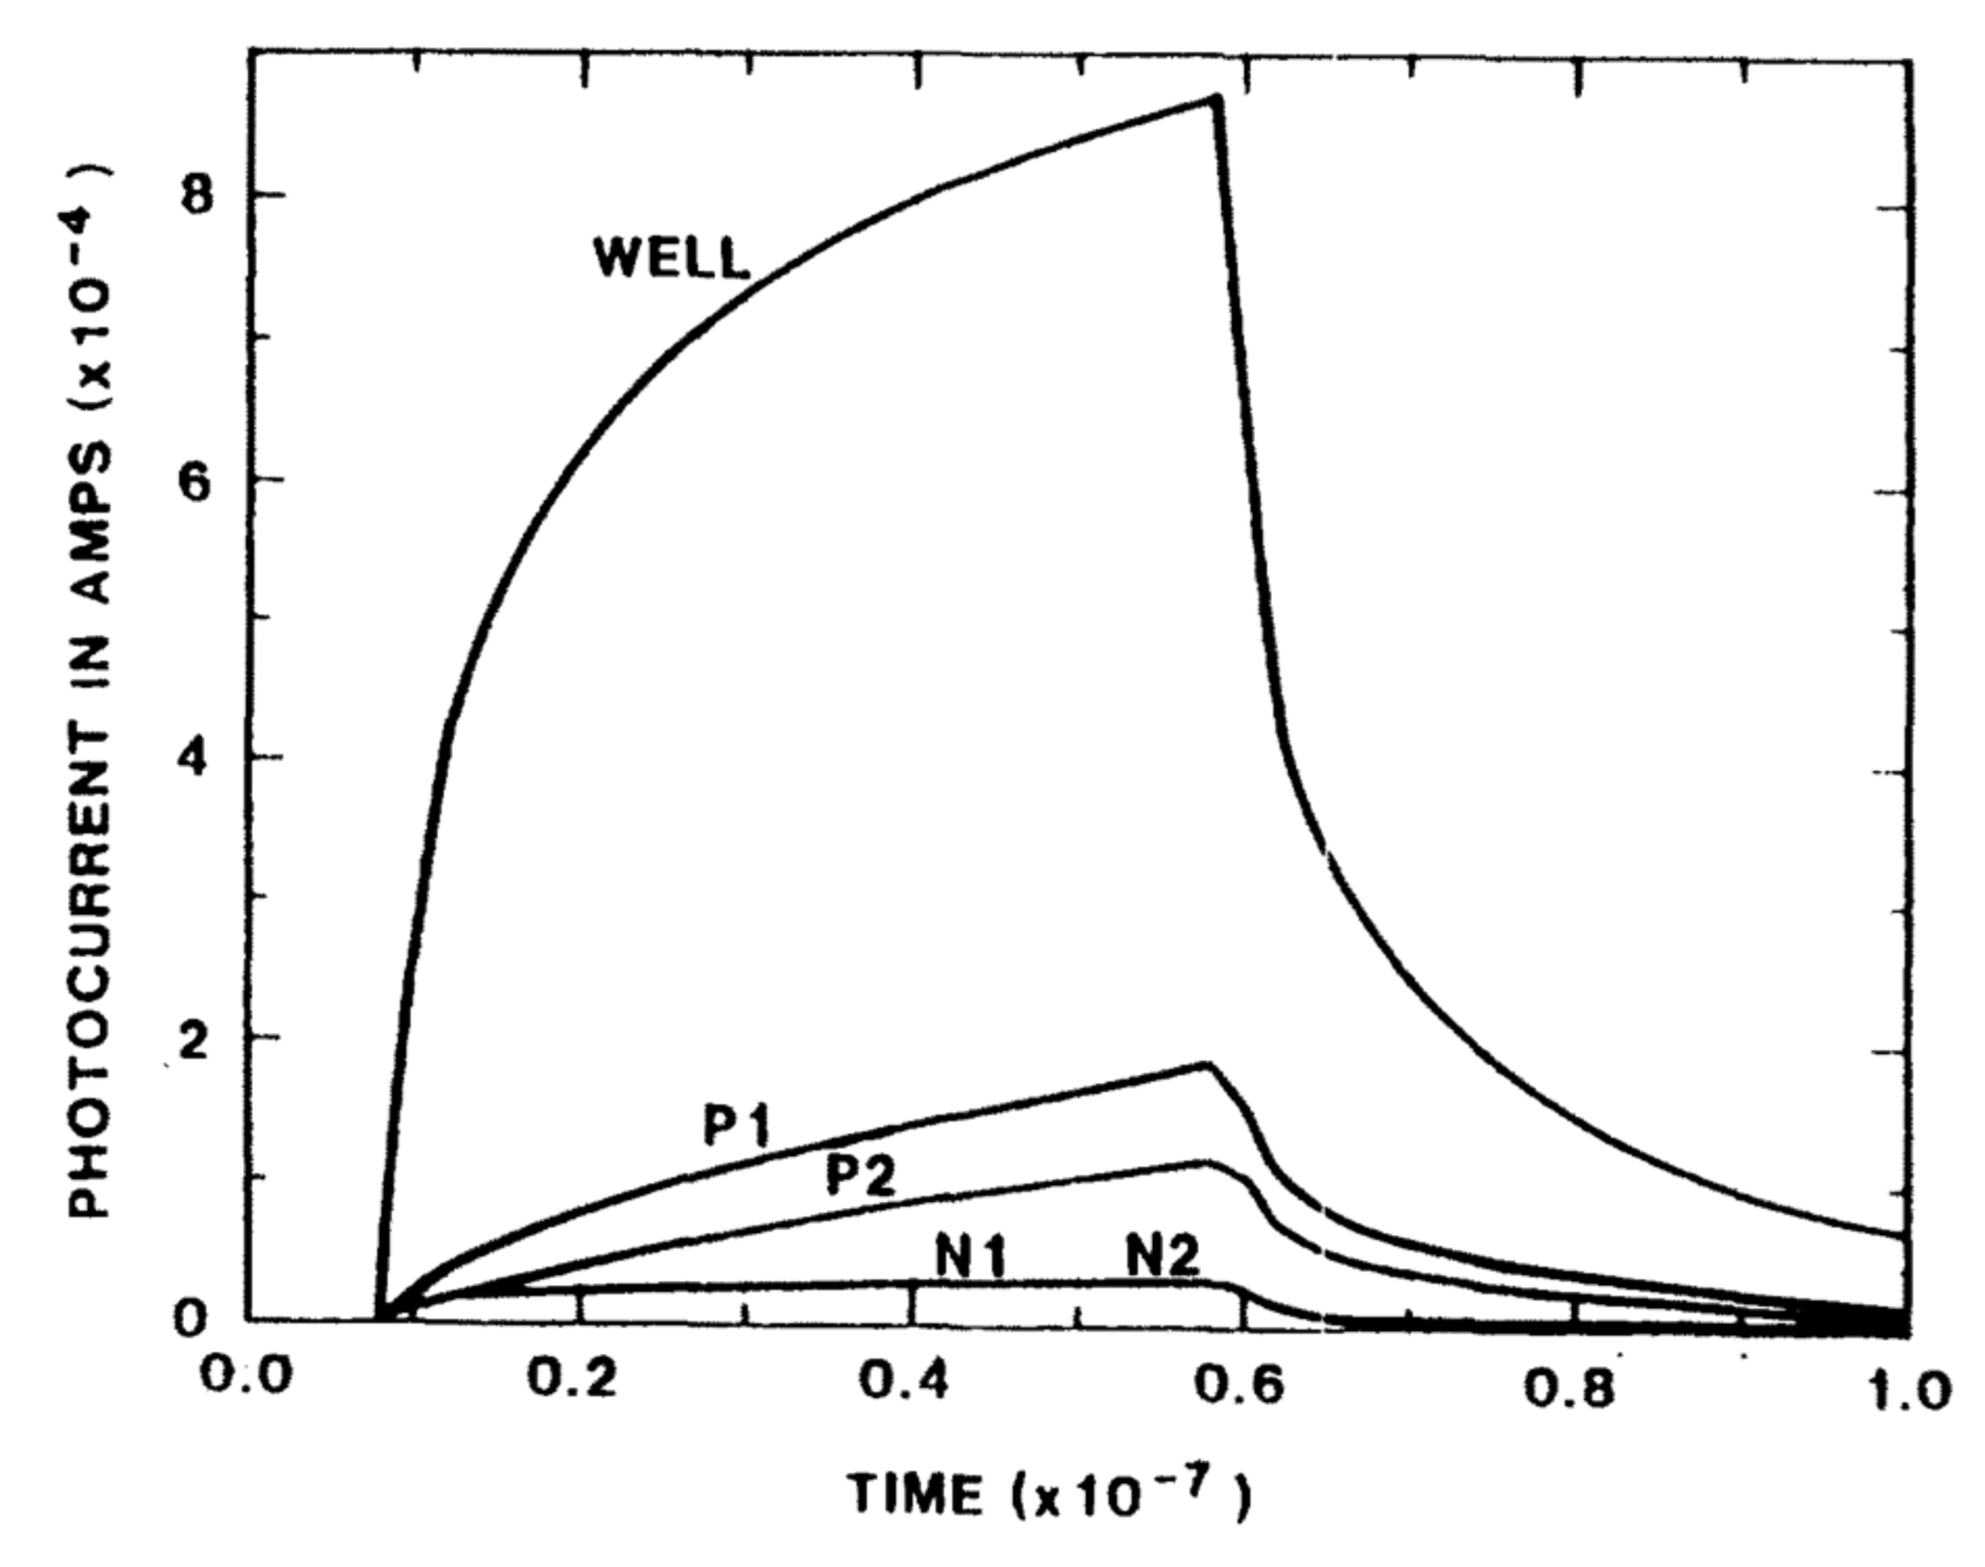
\includegraphics[width=4in]{photocurrents_local_well.pdf}
            \label{fig:photocurrents_sram_epi}
            }
    \end{center}
    \caption[Photocurrent waveforms, at a dose rate of 5$\times$10$^9$ rad(Si)/sec for the (a) bulk and (b) epi cases.]{Photocurrent waveforms, at a dose rate of 5$\times$10$^9$ rad(Si)/sec for the (a) bulk and (b) epi cases \cite{Massengill:1984hn}.}
    \label{fig:photocurrents_sram}
\end{figure}
Fig.~\ref{fig:photocurrents_sram} plots the photocurrent produced at the drain nodes and \emph{p}-well within an SRAM cell resulting from transient irradiation corresponding to a dose-rate of 5~Grad(Si)/sec.
The largest photocurrents clearly correspond to the \emph{p}-well contact in both the bulk~(\ref{fig:photocurrents_sram_bulk}) and epitaxial~(\ref{fig:photocurrents_sram_epi}) cases.
These photocurrents, which occur in every device across the entire chip, contribute to a non-negligible increase in power supply current.

Fig.~\ref{fig:photocurrents_sram} shows that errors occuring in a single SRAM cell are unlikely to be a local effect, since the magnitude of transients corresponding to the drain nodes within the SRAM cell are significantly smaller than the well photocurrent.
Instead, the onset of upsets resulting from transient irradiation of an SRAM test chip are related to the collective photocurrent of each well contact on the test chip \cite{Massengill:1984hn}.
This is due to the finite resistance of metal interconnects, the resulting photocurrents cause a voltage drop in $V_{DD}$ and an increase in $V_{SS}$ across the entire test chip. 
The resulting decrease in rail voltage ($V_{DD}$-$V_{SS}$) results in a higher than expected SRAM sensitivity to errors during transient irradiation \cite{Massengill:1984hn}.
\begin{figure}[htbp]
    \begin{center}
        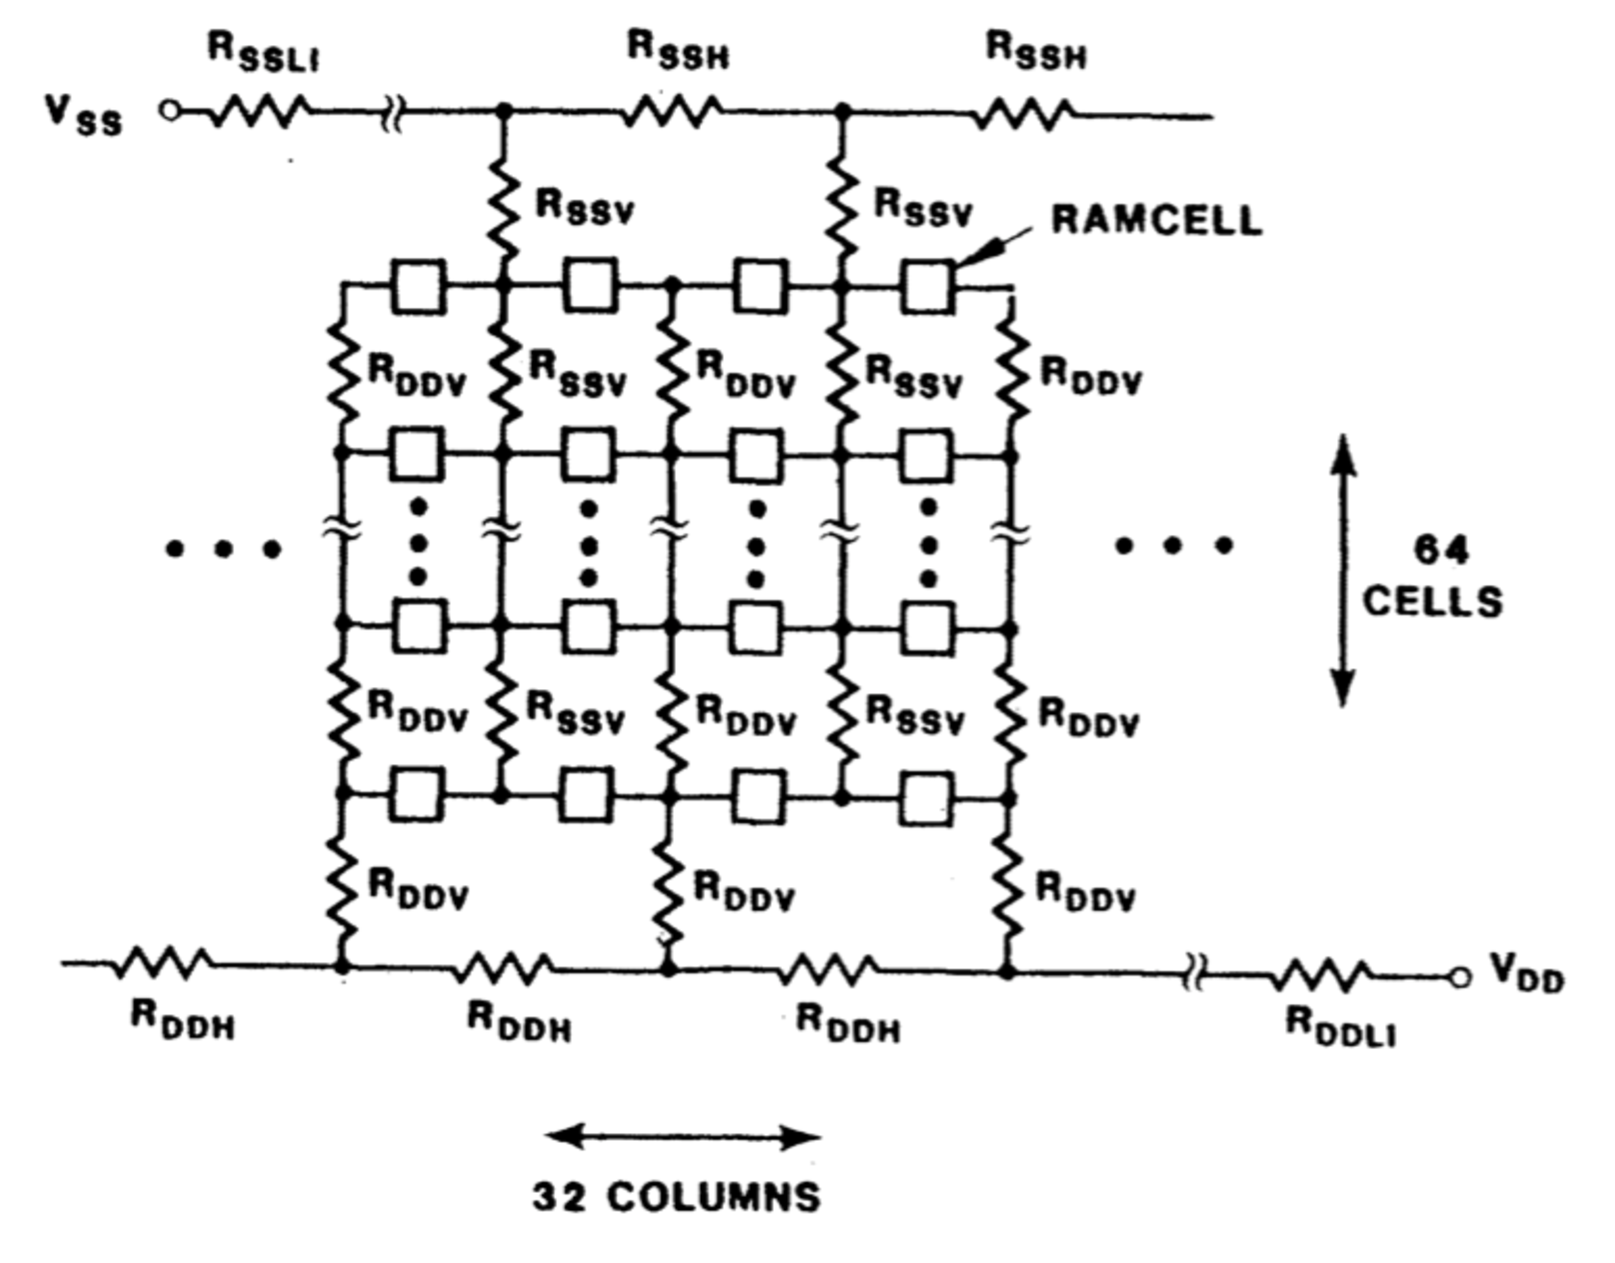
\includegraphics[width=4.5in]{SRAM_array_interconnect_resistance.pdf}
    \end{center}
    \caption[Schematic representation of the power distribution with the SRAM cells shown as ``black boxes''.]{Schematic representation of the power distribution with the SRAM cells shown as ``black boxes'' \cite{Massengill:1984hn}.}
    \label{fig:array_inter_resist}
\end{figure}
An example of the equivalent circuit diagram of an SRAM cell including interconnect resistances for $V_{DD}$ and $V_{SS}$ is shown in Fig.~\ref{fig:array_inter_resist}.
The resistances shown in parallel are labeled $R_{DDV}$ and $R_{SSV}$ corresponding to the finite resistance drop between individual SRAM cells on the high and low voltage rails, respectively.
Because the highest photocurrents are associated with charge collection on the \emph{p}-well node of an SRAM cell, the largest change in supply voltage occurs for SRAM cells furthest from the $V_{SS}$ supply lines \cite{Massengill:1984hn,Massengill:1985gd,Massengill:1986kp}.

Ultimately, it is the SRAM cells furthest from the $V_{SS}$ supply lines that are most sensitive under transient irradiation conditions.
\begin{figure}[htbp]
    \begin{center}
        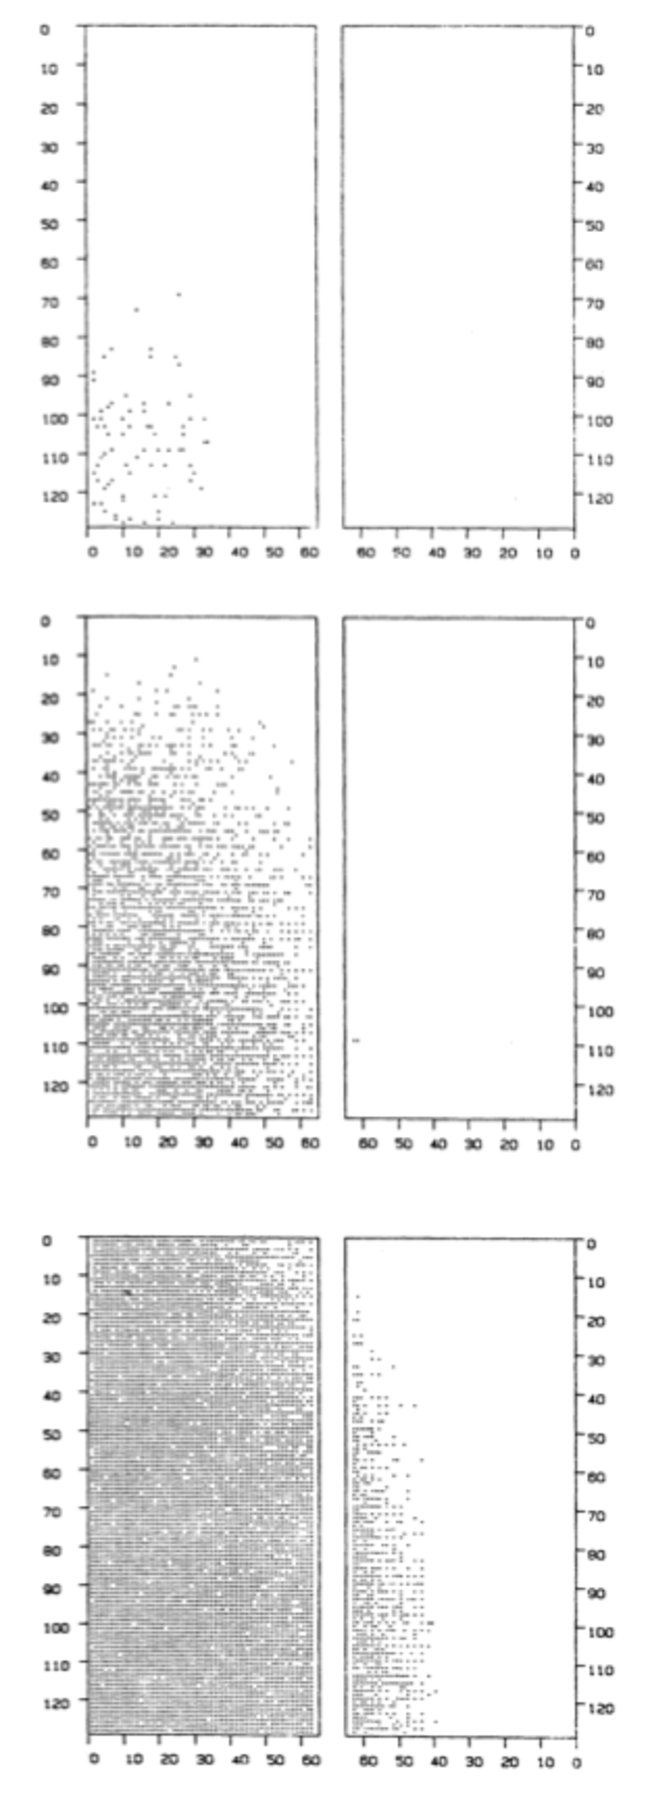
\includegraphics[height=6in]{mass_vss_railspan_collapse_bitmap.pdf}
    \end{center}
    \caption{Upset bit-map with no pre-test total dose for (a) 1.02$\times$10$^9$,(b)1.08$\times$10$^9$ and (c)1.16$\times$10$^9$ rad(Si)/sec.}
    \label{fig:railspan_coll_bit_map}
\end{figure}
This can be seen in Fig.~\ref{fig:railspan_coll_bit_map} where the lower left corner of the presented bit-map corresponds to SRAM bit locations furtherest from the the $V_{SS}$ supply line.
The SRAM test chips were exposed to dose-rates of 1.02$\times$10$^9$, 1.08$\times$10$^9$, and 1.16$\times$10$^9$ rad(Si)/sec.
The increased density of bit-errors near the lower-left corner of the test chip indicates that railspan collapse is the dominant mechanism contributing to upsets under these experimental conditions.
It is important to note that the dose-rates used in transient radiation experiments (on the order of Grad(Si)/sec) are \emph{extremely} high and do not represent typical dose-rates in either the space radiation or terrestrial environments (outside of the specific environments mentioned previously).
The signature of errors corresponding to railspan collapse, clusters of errors far from the $V_{SS}$ supply line, is useful for easily identifying the physical mechanism contributing to errors in SRAM experiments.
% subsection railspan_collapse (end)

% section radiation_effects_on_sram (end)

\section{Radiation Environments} % (fold)
\label{sec:radiation_environments}
Understanding the sources of ionizing radiation and modeling fluctuations in the concentration and flux of particle species is essential for accurately predicting error rates in modern electronics in the space radiation environment.
Table~\ref{table:rad_env} shows some important characteristics for the predominant particle species present in some of the common space radiation environments.
Each of these environments has unique signature in terms of the species, the energy, and the flux of those particles present.
Consequently, the presence of radiation in each environment has specific implications for electronics unique to those environments.
The CREME96 \cite{tylka1997creme96} and CR\`EME-MC \cite{keys2008review,sierawski2010creme} codes exist as a means to provide critical information regarding the environments shown in Table~\ref{table:rad_env}.
The use of these codes provides a rudimentary framework for evaluating the potential risk of flying certain types of microelectronics in the different environments.
The following section addresses the particle species present in each environment and their impact on electronic systems.
\begin{table}[htbp]
    \caption[Particle Radiations in Near-Earth Orbit and Some Properties]{Particle Radiations in Near-Earth Orbit and Some Properties \cite{Xapsos:2013cu}}
    \centering
        \begin{tabular}{C{0.75in}|C{1.1in}C{1.1in}C{1.1in}C{1.1in}}
        \hline\hline
        Radiation & Maximum Energy & Maximum Flux & Radiation Effects & Shielding Effectiveness \\
        \hline\hline
        Earth Trapped Protons & 500~MeV & 10$^5$ cm$^{-2}$ s$^{-1}$ & TID, DD, SEE & Moderate \\
        \hline
        Earth Trapped Electrons & 10~MeV & 10$^6$ cm$^{-2}$ s$^{-1}$ & TID, DD, ESD & High\\ \hline
        Jovian Trapped Electrons & 100~MeV & 10$^9$ cm$^{-2}$ s$^{-1}$ & TID, DD, ESD & High\\ \hline
        Galactic Cosmic Rays & 10$^{11}$ GeV & 10 cm$^{-2}$ s$^{-1}$ & SEE & Low \\ \hline
        Solar Particle Events & 10 GeV/n & 10$^5$ cm$^{-2}$ s$^{-1}$ & TID, DD, SEE & Moderate \\\hline\hline
        \end{tabular}
        \label{table:rad_env}
    %\end{centering}
\end{table}

\subsection{Solar Particle Environment} % (fold)
\label{sub:solar_wind}
Solar particle events result in the ejection of large quantity of relatively low energy charged emitted from the sun into interplanetary space.
There are two types of solar particle events, solar flares and coronal mass ejections (CME), each of which have distinct signatures and release energetic particles.
Solar flares occur when energy stored in the coronal magnetic field becomes too large and releases a burst of energy, which in turn accelerates charged particles away from the sun.
Such events tend to last for hours and emit a large measure of charged particles.
The particle species present are frequently electron rich, though protons and helium ions are also present in solar flares \cite{xapsos:2006}.
A CME is a release of plasma, consisting of free electrons and ions, the shock wave accelerates particles outward into interplanetary space.
CMEs tend to be proton rich and last for several days.
The dominant interaction mechanisms of electronics with particles in the solar particle environment are TID, displacement damage, and SEEs.
Of the two types of solar particle events, CMEs are responsible for major disruptions in interplanetary space and large scale geomagnetic disturbances on earth that can in turn result in disruption of communications and electronics.

\begin{figure}[htbp]
    \begin{center}
        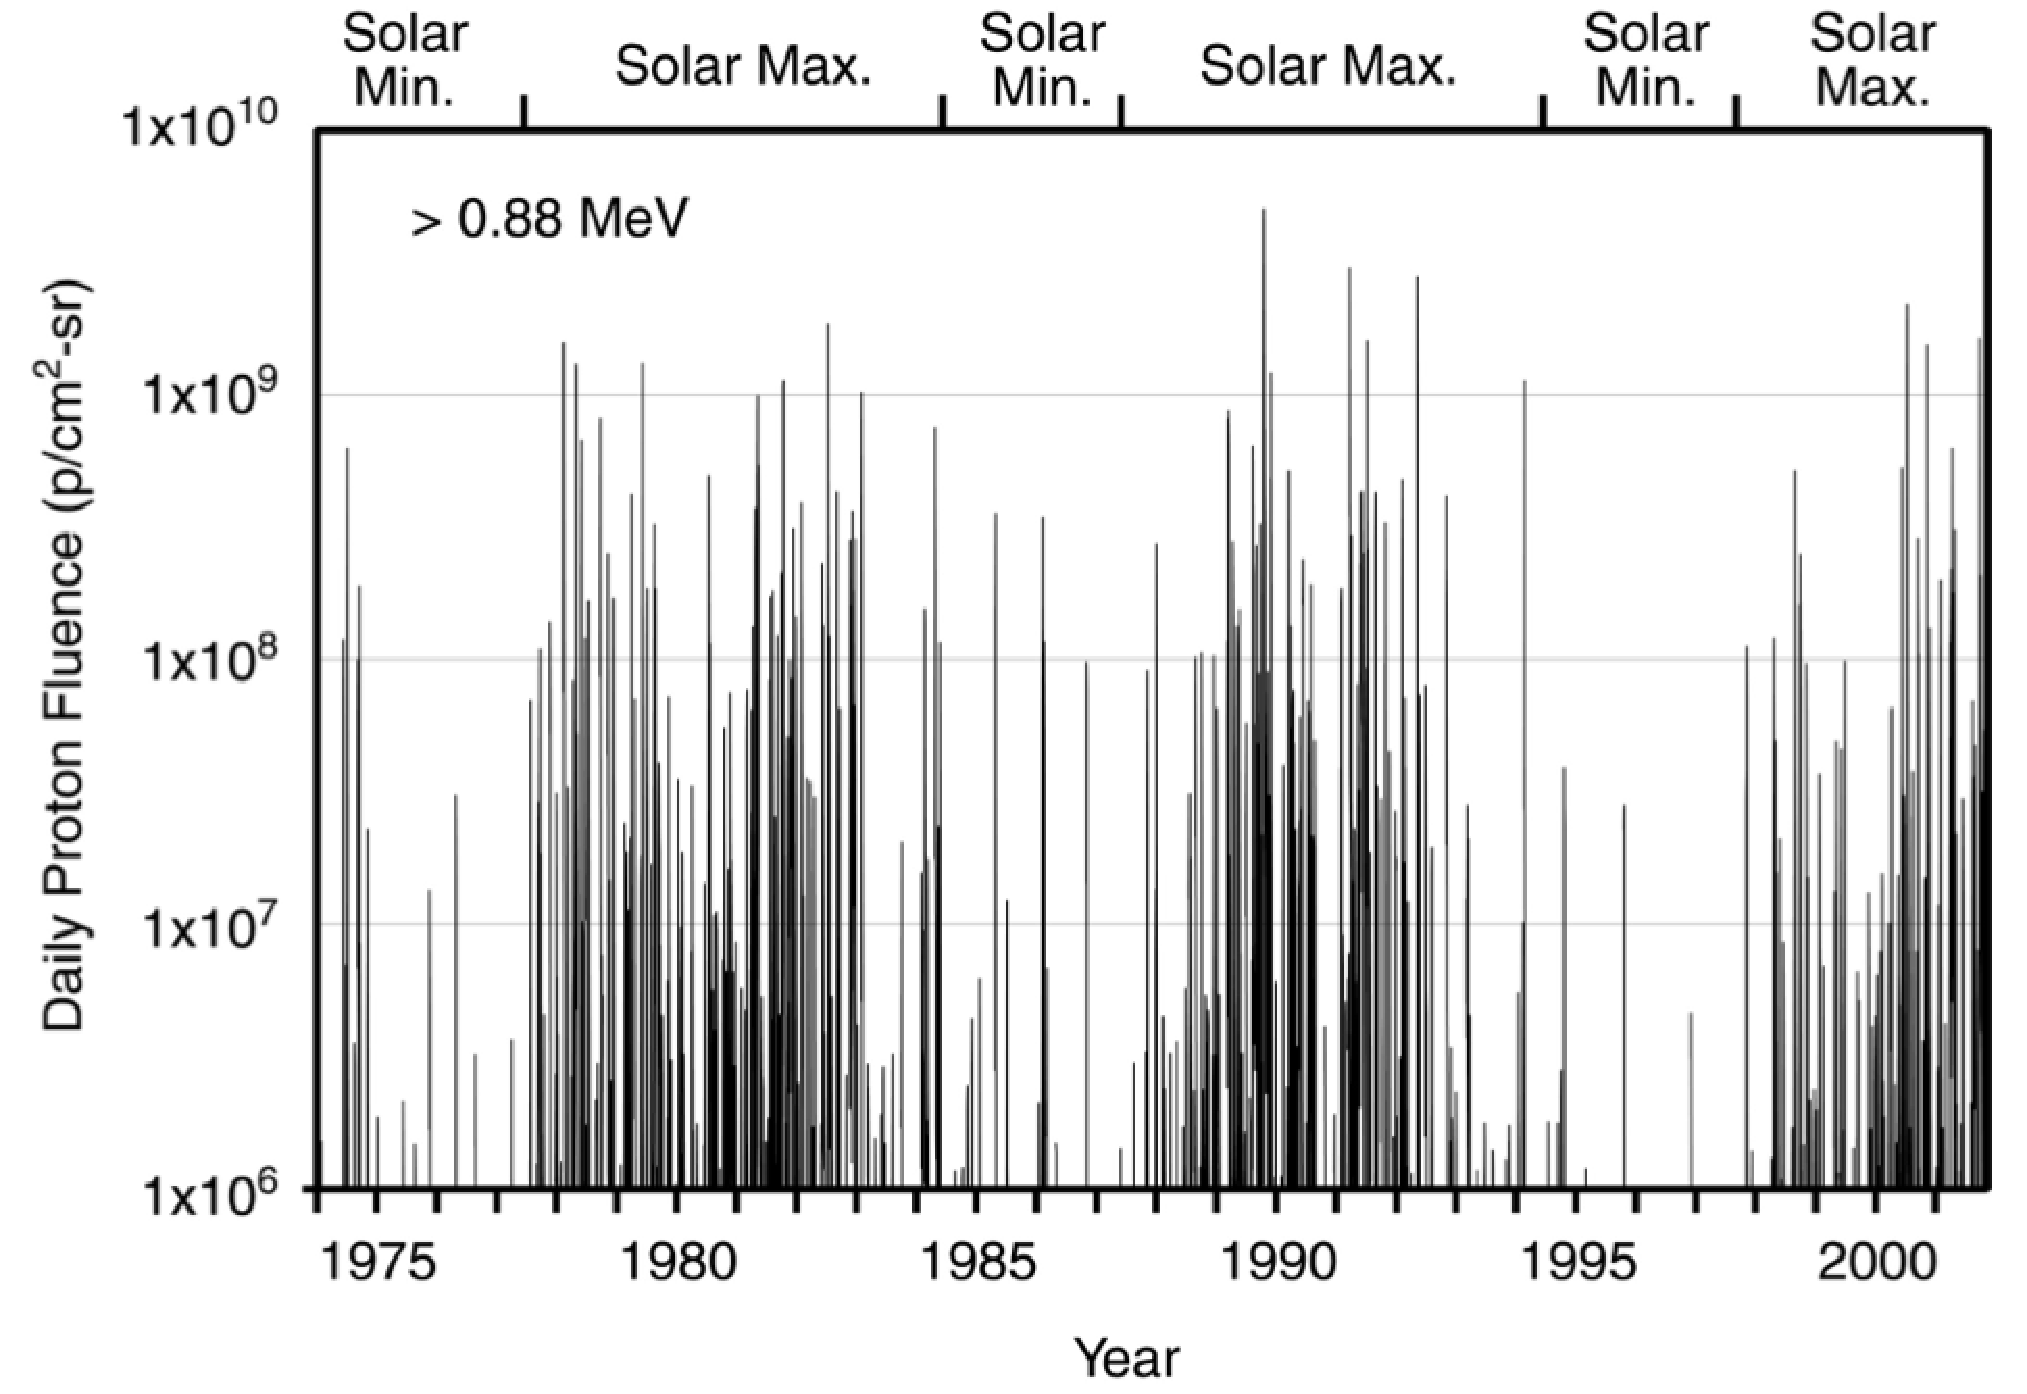
\includegraphics[width=5in]{xapsos_proton_fluence_vs_year_SPE.pdf}
    \end{center}
    \caption[Daily fluences of $>$ 0.88 MeV protons due to solar particle events between approximately 1974 and 2002.]{Daily fluences of $>$ 0.88 MeV protons due to solar particle events between approximately 1974 and 2002 \cite{xapsos:2006}.}
    \label{fig:proton_fluence_vs_year}
\end{figure}

All naturally occuring elements are present in solar particle events at some detectable level of concentration, although they consist primarily ($>$ 99.9\%) of solar protons, helium, and electrons.
Despite the small composition the presence of heavy ions in the solar particle environment is a non-negligible population of particle species, particularly when evaluating the impact of radiation on electronics.
Solar particle events have been observed to vary over time with fairly predictable intervals where activity levels are at a minimum and maximum.
A plot of daily solar proton fluence can be seen in Fig.~\ref{fig:proton_fluence_vs_year}.
The CREME96 models were adapted to account for variations in solar activity and provide accurate representation of particle fluxes present in the near-earth environment.
Fig.~\ref{fig:spe-geo-worst-day-100-mils} shows the particle flux spectra from CREME96 for a geosynchronous orbit during ``worst-day'' conditions with 100~mils of aluminum shielding \cite{tylka1997creme96}.
Particle energies in solar flares and CME events may approach 1~GeV/u with peak fluxes higher than 10$^5$~cm$^{-2}$~s$^{-1}$.
\begin{figure}[htbp]
    \begin{center}
        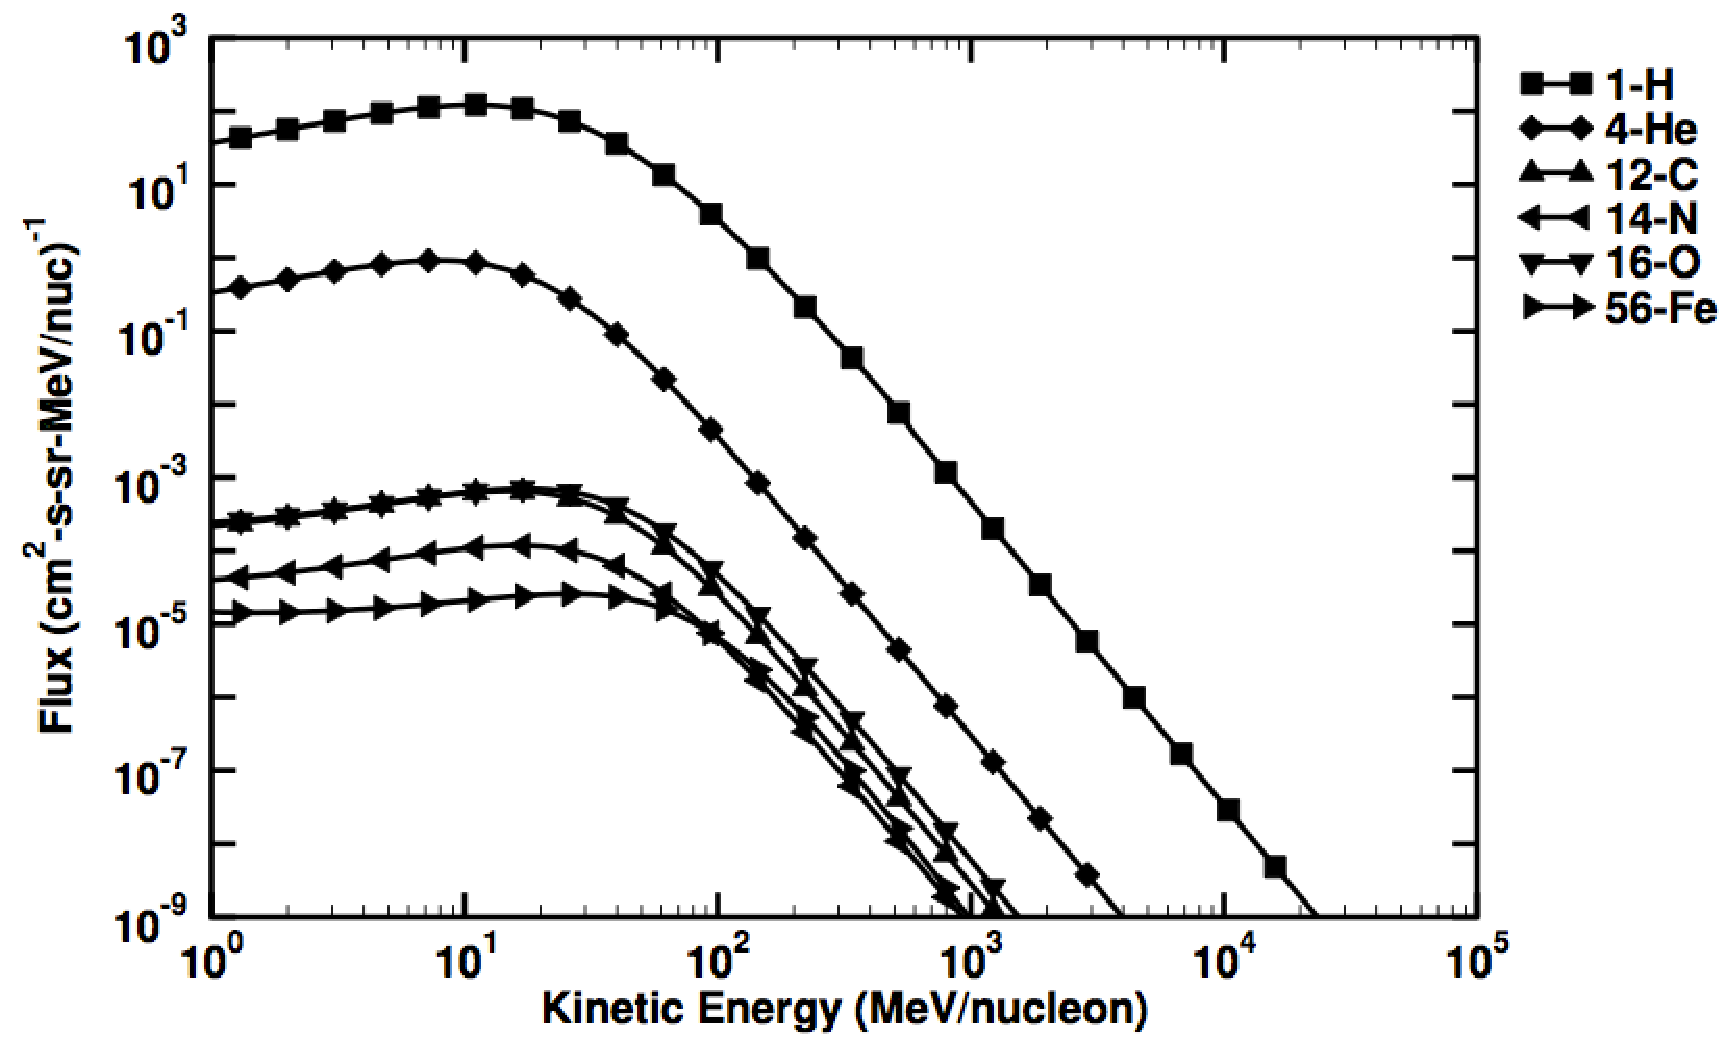
\includegraphics[width=5in]{sierawski_spe_geo_worst_day_100_mils.pdf}
    \end{center}
    \caption[The particle flux spectra computed by CREME96 for a Near-Earth Interplanetary or Geosynchronous orbit during the worst day scenario with 100 mils of aluminum shielding. Common species shown, all others omitted.]{The particle flux spectra computed by CREME96 for a Near-Earth Interplanetary or Geosynchronous orbit during the worst day scenario with 100 mils of aluminum shielding. Common species shown, all others omitted \cite{Sierawski:2011tc}.}
    \label{fig:spe-geo-worst-day-100-mils}
\end{figure}
% subsection solar_wind (end)

\subsection{Galactic Cosmic Rays} % (fold)
\label{sub:galactic_cosmic_rays}
Galactic cosmic rays (GCR) are high-energy particles, primarily hadrons, that originate from outside our solar system.
These energetic, charged particles are stripped of electrons by the interstellar medium and accelerated to high energies.
The primary concern for microelectronic systems exposed to the GCR environment are SEEs.

A basic description of the GCR environment is given in Table~\ref{table:rad_env}.
All naturally occurring elements are present in the GCR environment up to uranium.
The particle spectrum is represented by approximately 90\% protons, 9\% helium, while heavier elements from lithium through iron and nickel make up the remaining 1\% of particle species.
A large decrease in abundance occurs for atomic numbers higher than iron, this feature of the GCR spectrum is known as the ``iron knee''.
The relative abundance of elements through Z=28 is shown in Fig.~\ref{fig:gcr-abundance-vs-atomic-num}.
\begin{figure}[htbp]
    \begin{center}
        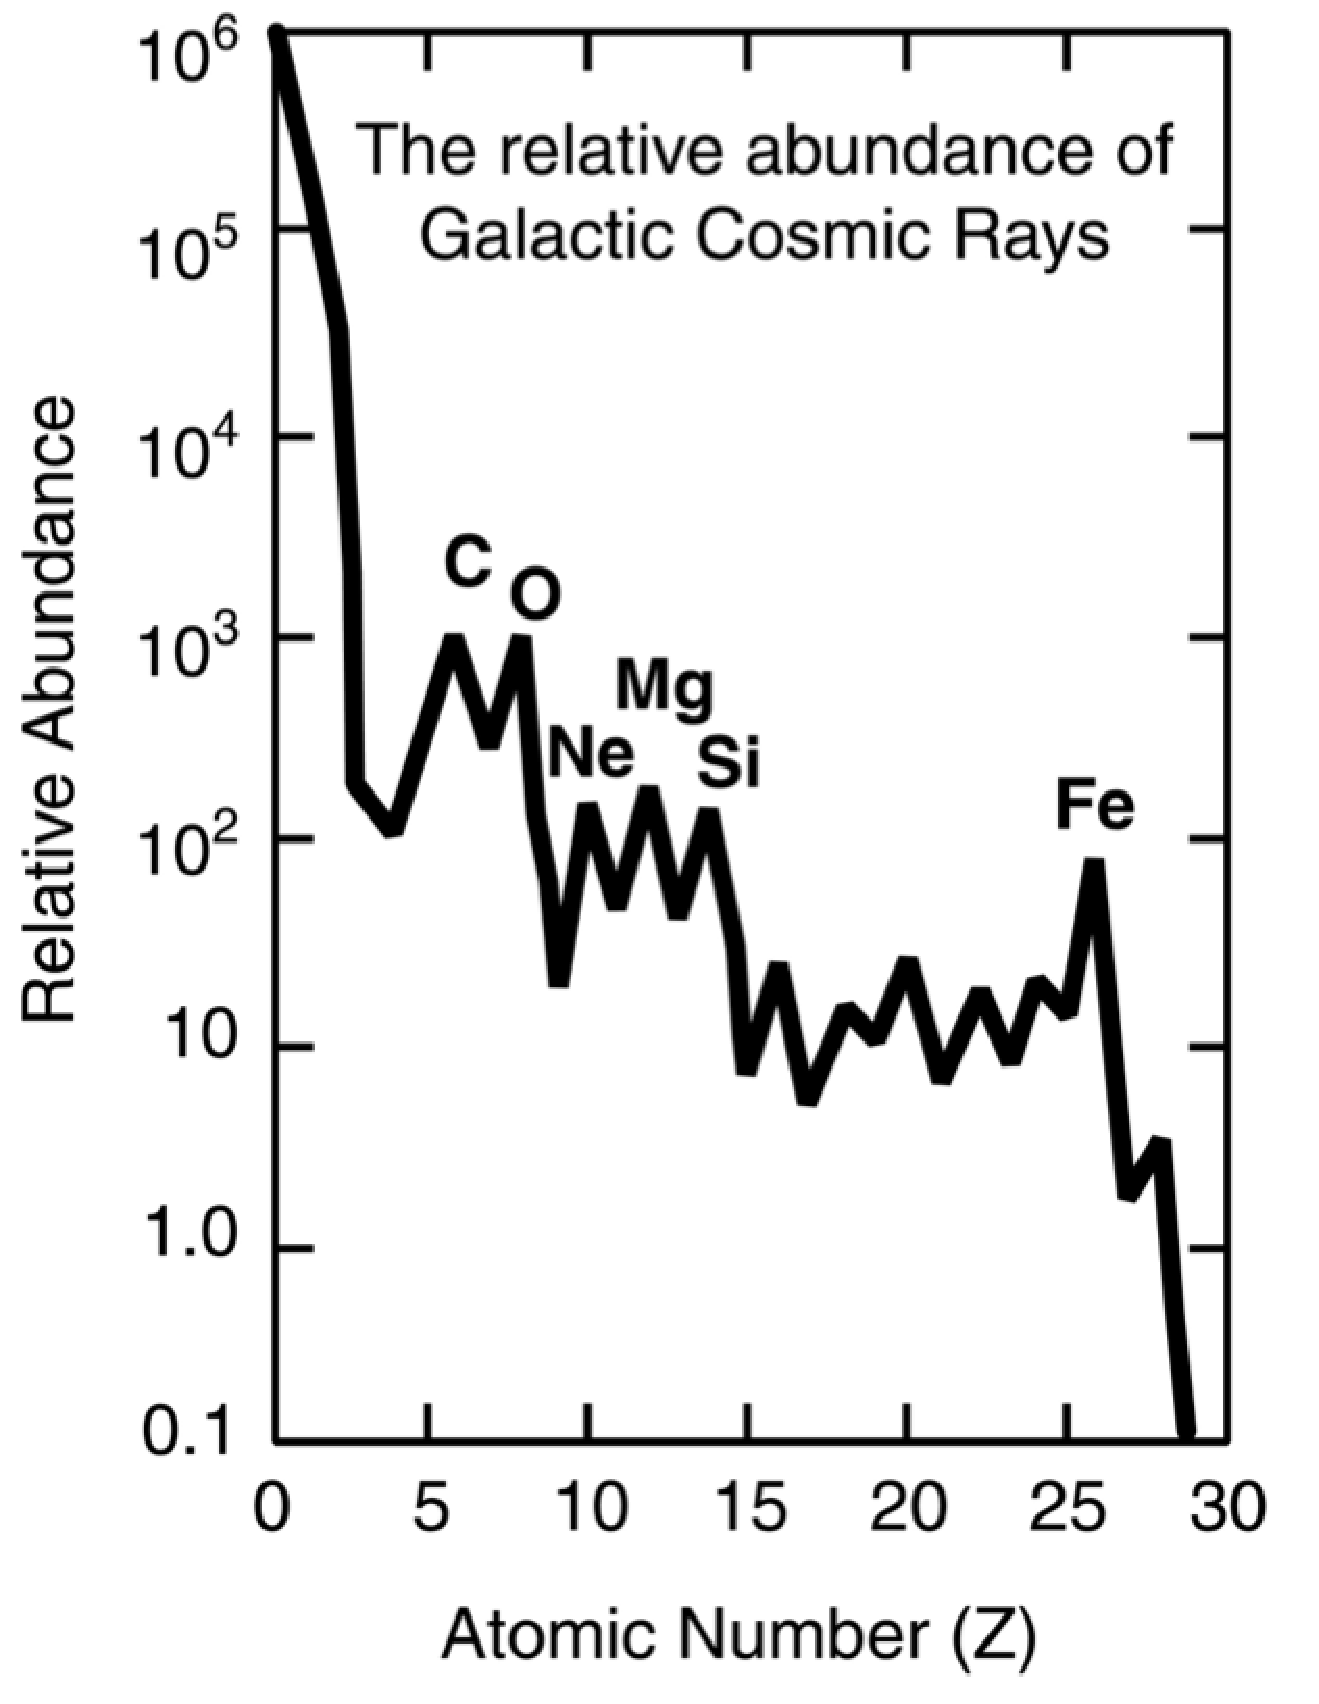
\includegraphics[height=6in]{xapsos-gcr-abundance-vs-atomic-num.pdf}
    \end{center}
    \caption[Abundances of particles species in the GCR spectrum up through Z = 28.]{Abundances of particles species in the GCR spectrum up through Z = 28 \cite{xapsos:2006}.}
    \label{fig:gcr-abundance-vs-atomic-num}
\end{figure}

The local interstellar medium is a relativity constant, isotropic flux at the heliosphere boundary.
The presence of a magnetic field from the sun impedes the flux of low-energy ($<$20~MeV/u) particles in the GCR spectrum entering the solar system.
Additionally, the solar wind modulates the flux of particles from the GCR in regions of interplanetary space.
Consequently, increased solar activity levels result in a lower flux of particles emanating from the GCR environment and lower solar activity levels result in an increase in the GCR flux in interplanetary space \cite{parker1965passage,badhwar1992improved}.
The impact of solar activity on the differential energy spectra of common elements in the GCR environment is shown in Fig.~\ref{fig:gcr-fluence-vs-energy}.
Together, the combination of solar particles and the GCR environment make up the interplanetary radiation environment.
The region of consideration for particles originating from these sources ranges from geosynchronous orbits to the free space between planets.

\begin{figure}[tb]
    \begin{center}
        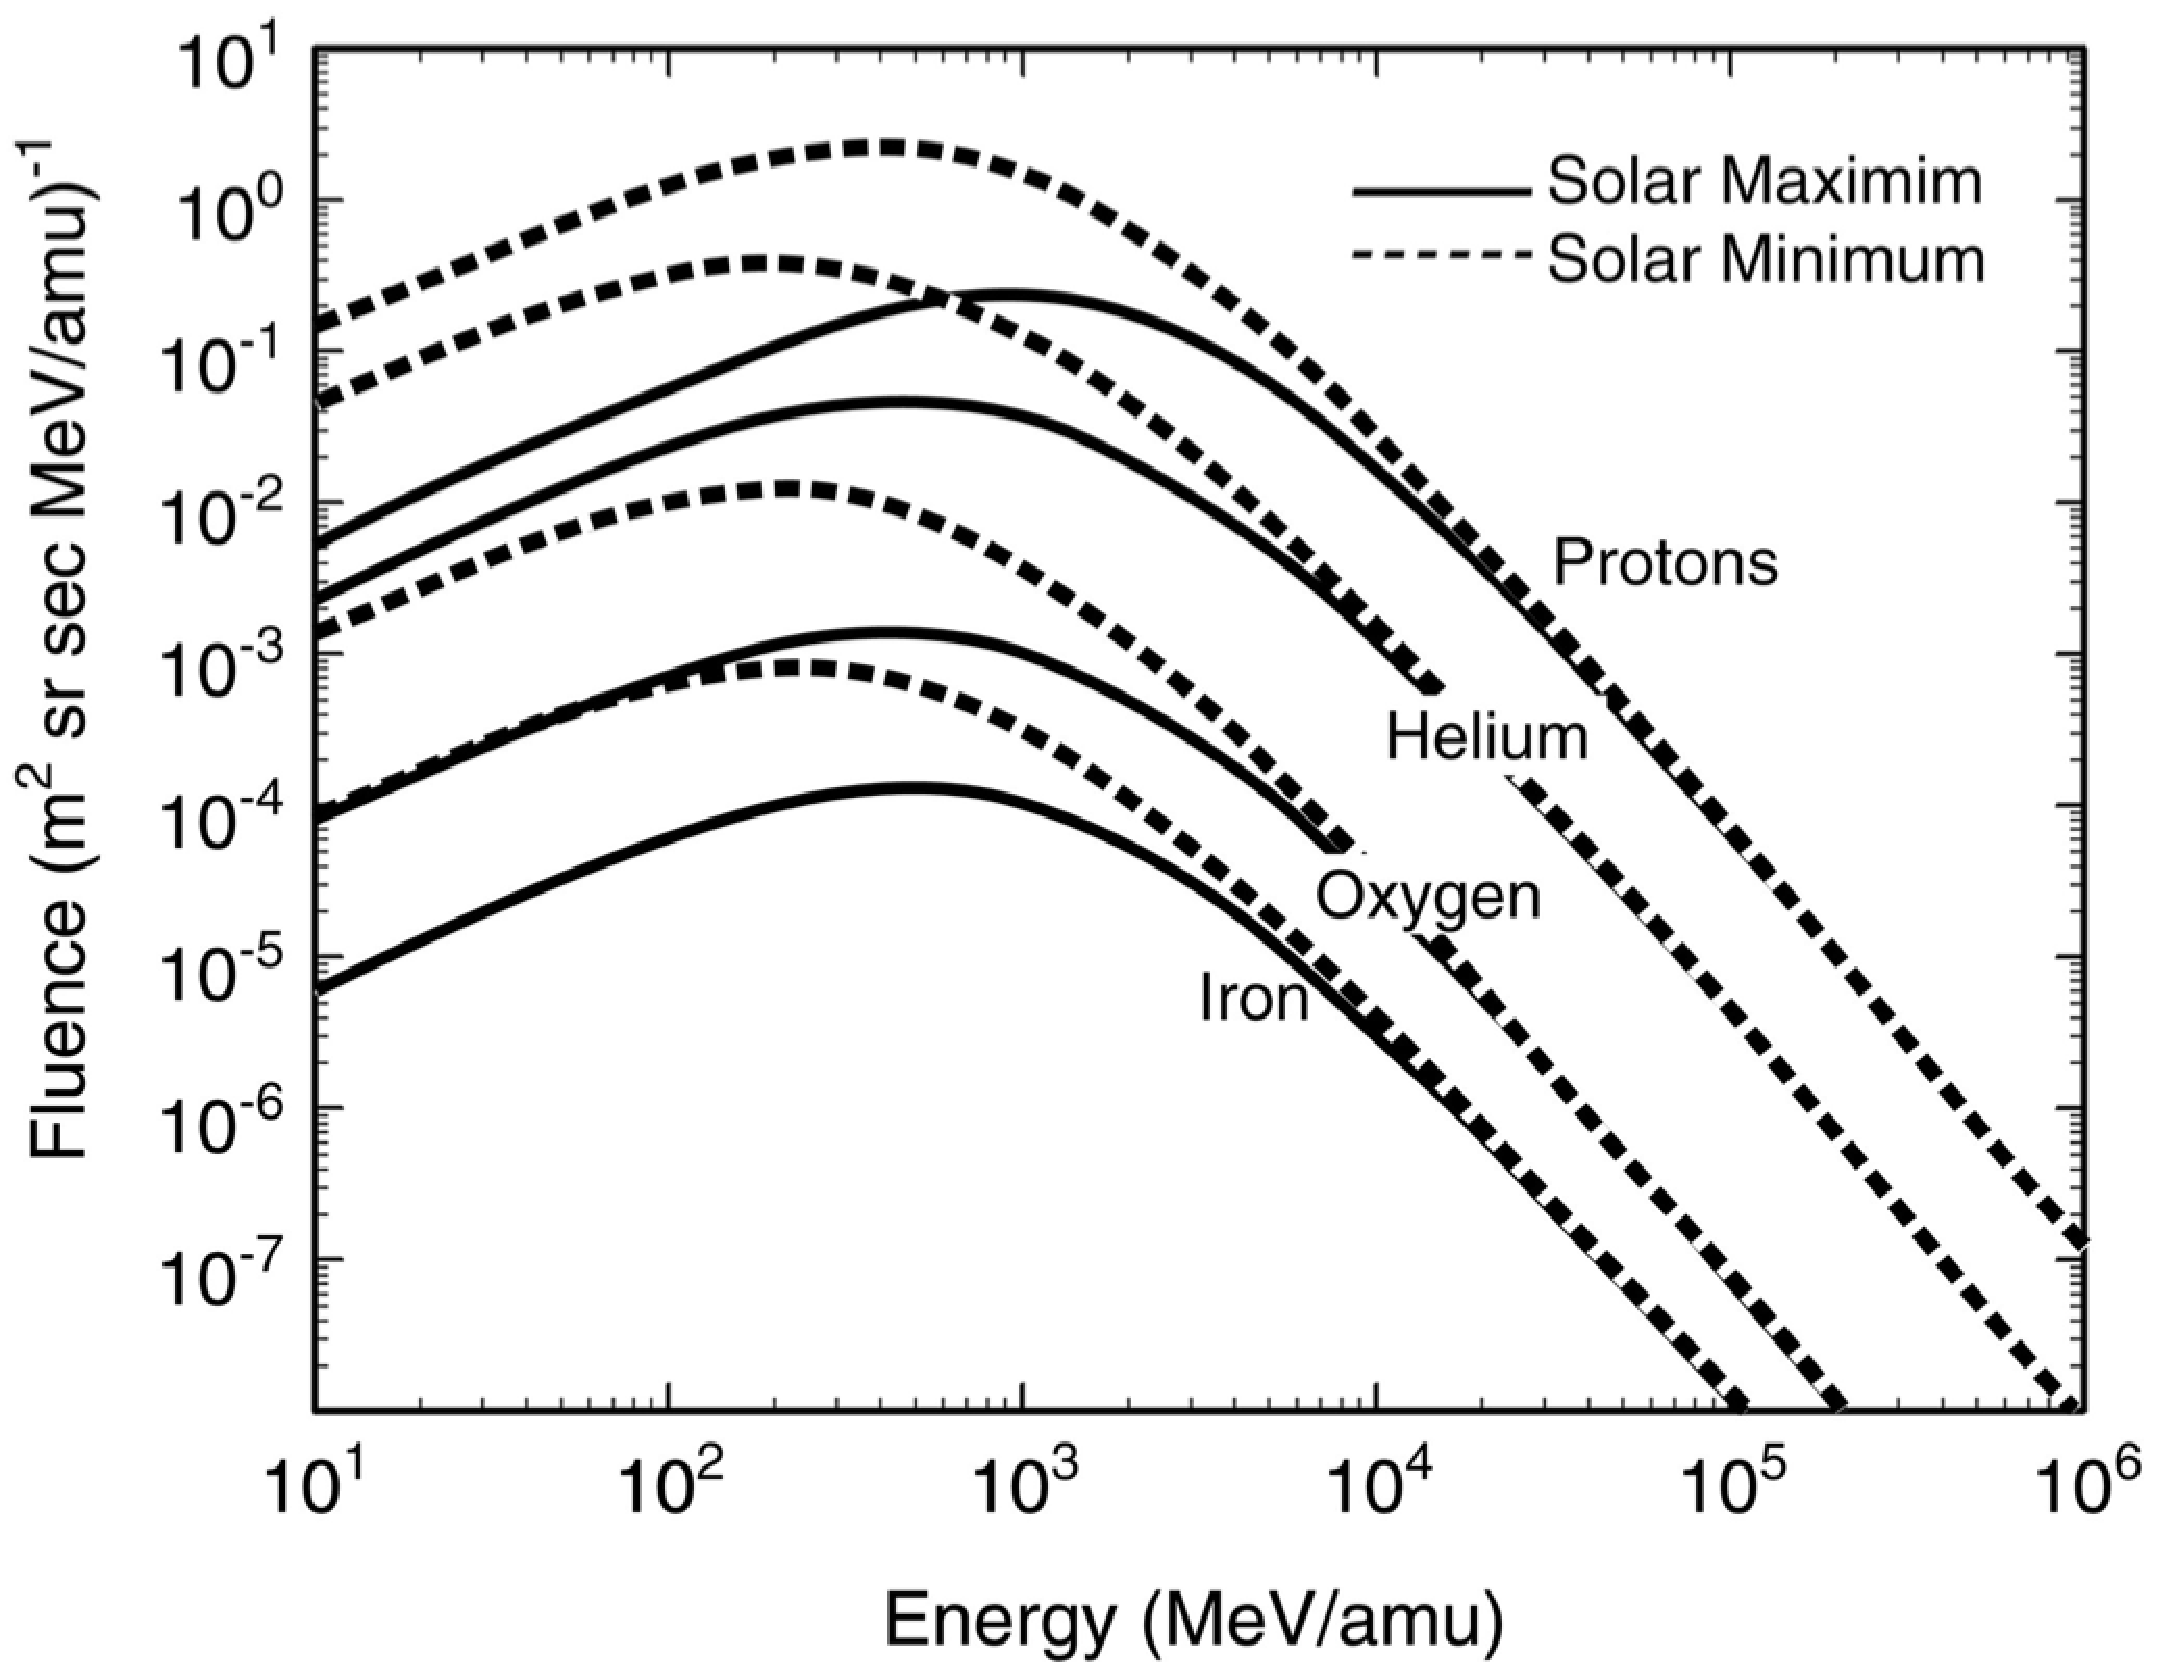
\includegraphics[width=5in]{xapsos_gcr_fluence_vs_energy.pdf}
    \end{center}
    \caption[GCR energy spectra for protons, helium, oxygen and iron during solar maximum and solar minimum conditions.]{GCR energy spectra for protons, helium, oxygen and iron during solar maximum and solar minimum conditions \cite{badhwar1996galactic}.}
    \label{fig:gcr-fluence-vs-energy}
\end{figure}

The CREME96 and CR\`EME-MC tools represent efforts attempting to provide a reliable framework for analyzing the susceptibility of modern electronics to particles from the GCR environment.
These codes provide a consistent metric for analyzing the flux and LET of particles exposed to the GCR environment and provide a means of analysis for estimating error/event rates.
% subsection galactic_cosmic_rays (end)

\subsection{Trapped Particle Environments} % (fold)
\label{sub:trapped_particle_environment}
Energetic charged particles are captured by and present around planets with significant magnetic fields.
Orbiting satellites, manned, and robotic space exploration missions encounter the trapped particle environment for the extent of the mission lifetime.
The near-Earth radiation environment is of primary importance for orbiting communications, weather, GPS, defense, and scientific satellites.
The near-Earth environment also has significance due to the presence of the international space station where mission criteria must additionally consider the biological and electronic impact of radiation on systems and the human presence on the ISS.

The Jovian environment is of interest to scientists and researchers interested in looking at geological processes on several of the moons.
To date, NASA has planned several future missions that send remote sensing satellite probes to the Jovian environment to investigate its moons, Io and Europa, in addition to studies of Jupiter itself.
The trapped particle environment around Jupiter is particularly difficult from a mission reliability perspective due to the presence of high-flux, high-energy charged particles trapped in the planets magnetosphere.

The following discussion will focus exclusively on the near-Earth environment and Jovian environment.

\subsubsection{Earth Radiation Belts} % (fold)
\label{ssub:van_allen_radiation_belts}
The Earth's magnetic field acts as a barrier to electromagnetic radiation but also acts to trap charged particles in stable orbits around the planet.
The regions where charged particles can be found around the planet are known as radiation belts.
The particles populating the radiation fields surrounding the Earth originate from solar particle events and the GCR environment, although for some time an ill-conceived high altitude nuclear weapons test referred to as operation Starfish Prime did introduce and modify the particle species and structure of the radiation belts.
The discovery of the radiation belts surrounding Earth is credited to Van Allen who performed the initial analysis of data identifying the particle populations and mapping their intensities \cite{van1959radiation}.
Since their discovery, additional studies of the trapped particle environments surrounding Earth have been performed, identifying the particle species present, flux, and variation in particle population based on solar and military activities \cite{sawyer1976ap,vette1991ae}.
The initial AE-8 and AP-8 models allowed designers to account for TID, SEE, displacement damage, and spacecraft charging effects.
As electronics have become increasingly sensitive to ionizing particle events it has become increasingly difficult to utilize the AE-8 and AP-8 models accurately.
Efforts continue to refine the trapped particle environment models to account for sources of error and uncertainty and much progress has been made for the AE-9 and AP-9 models \cite{barth2003space,Xapsos:2013cu,Bourdarie:kj}.

A basic description of common particles found in the trapped particle environment can be seen in Table~\ref{table:rad_env}.
Trapped electrons, protons, and alpha particles are the majority particle populations, making up greater than 99.9\% of particle species \cite{xapsos:2006}. 
These particles are separated into two regions, an inner and outer radiation belt, with a ``lower'' flux slot region between.
Contour plots of the particle populations for electrons and protons can be seen in Figs.~\ref{fig:earth-trapped-electrons} and \ref{fig:earth-trapped-protons}, respectively.
\begin{figure}[htbp]
    \begin{center}
        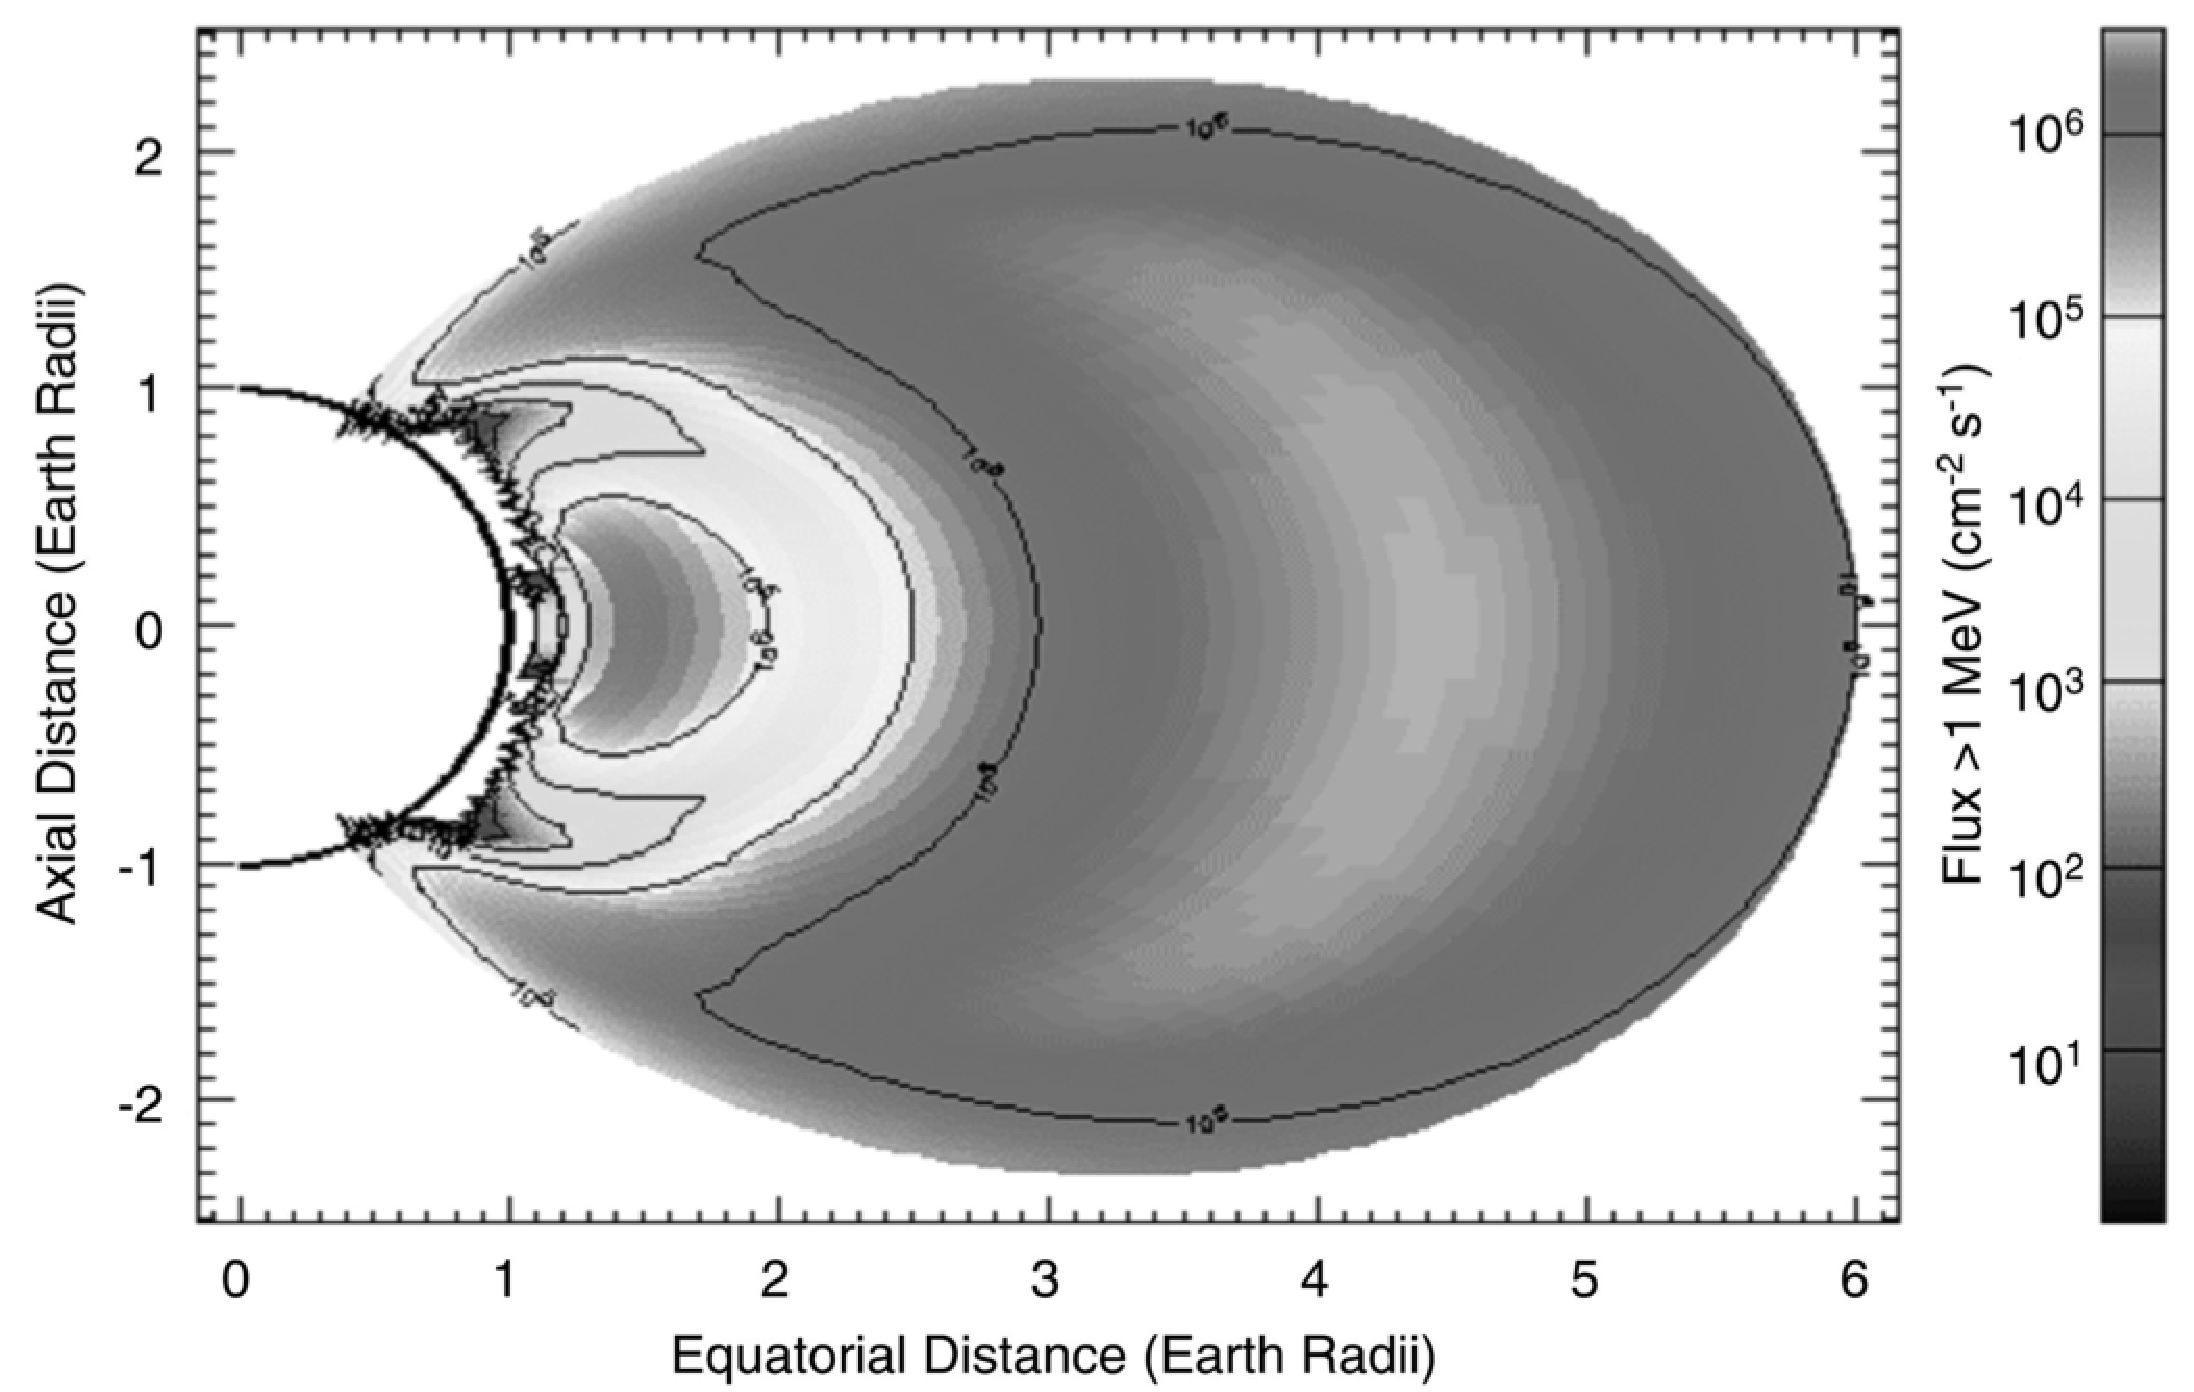
\includegraphics[width=5in]{xapsos_elec_spec_earth.pdf}
    \end{center}
    \caption[The electron population with energies $>$ 1 MeV as predicted by the AE-8 model for solar maximum conditions.]{The electron population with energies $>$ 1 MeV as predicted by the AE-8 model for solar maximum conditions \cite{xapsos:2006}.}
    \label{fig:earth-trapped-electrons}
\end{figure}
\begin{figure}[htbp]
    \begin{center}
        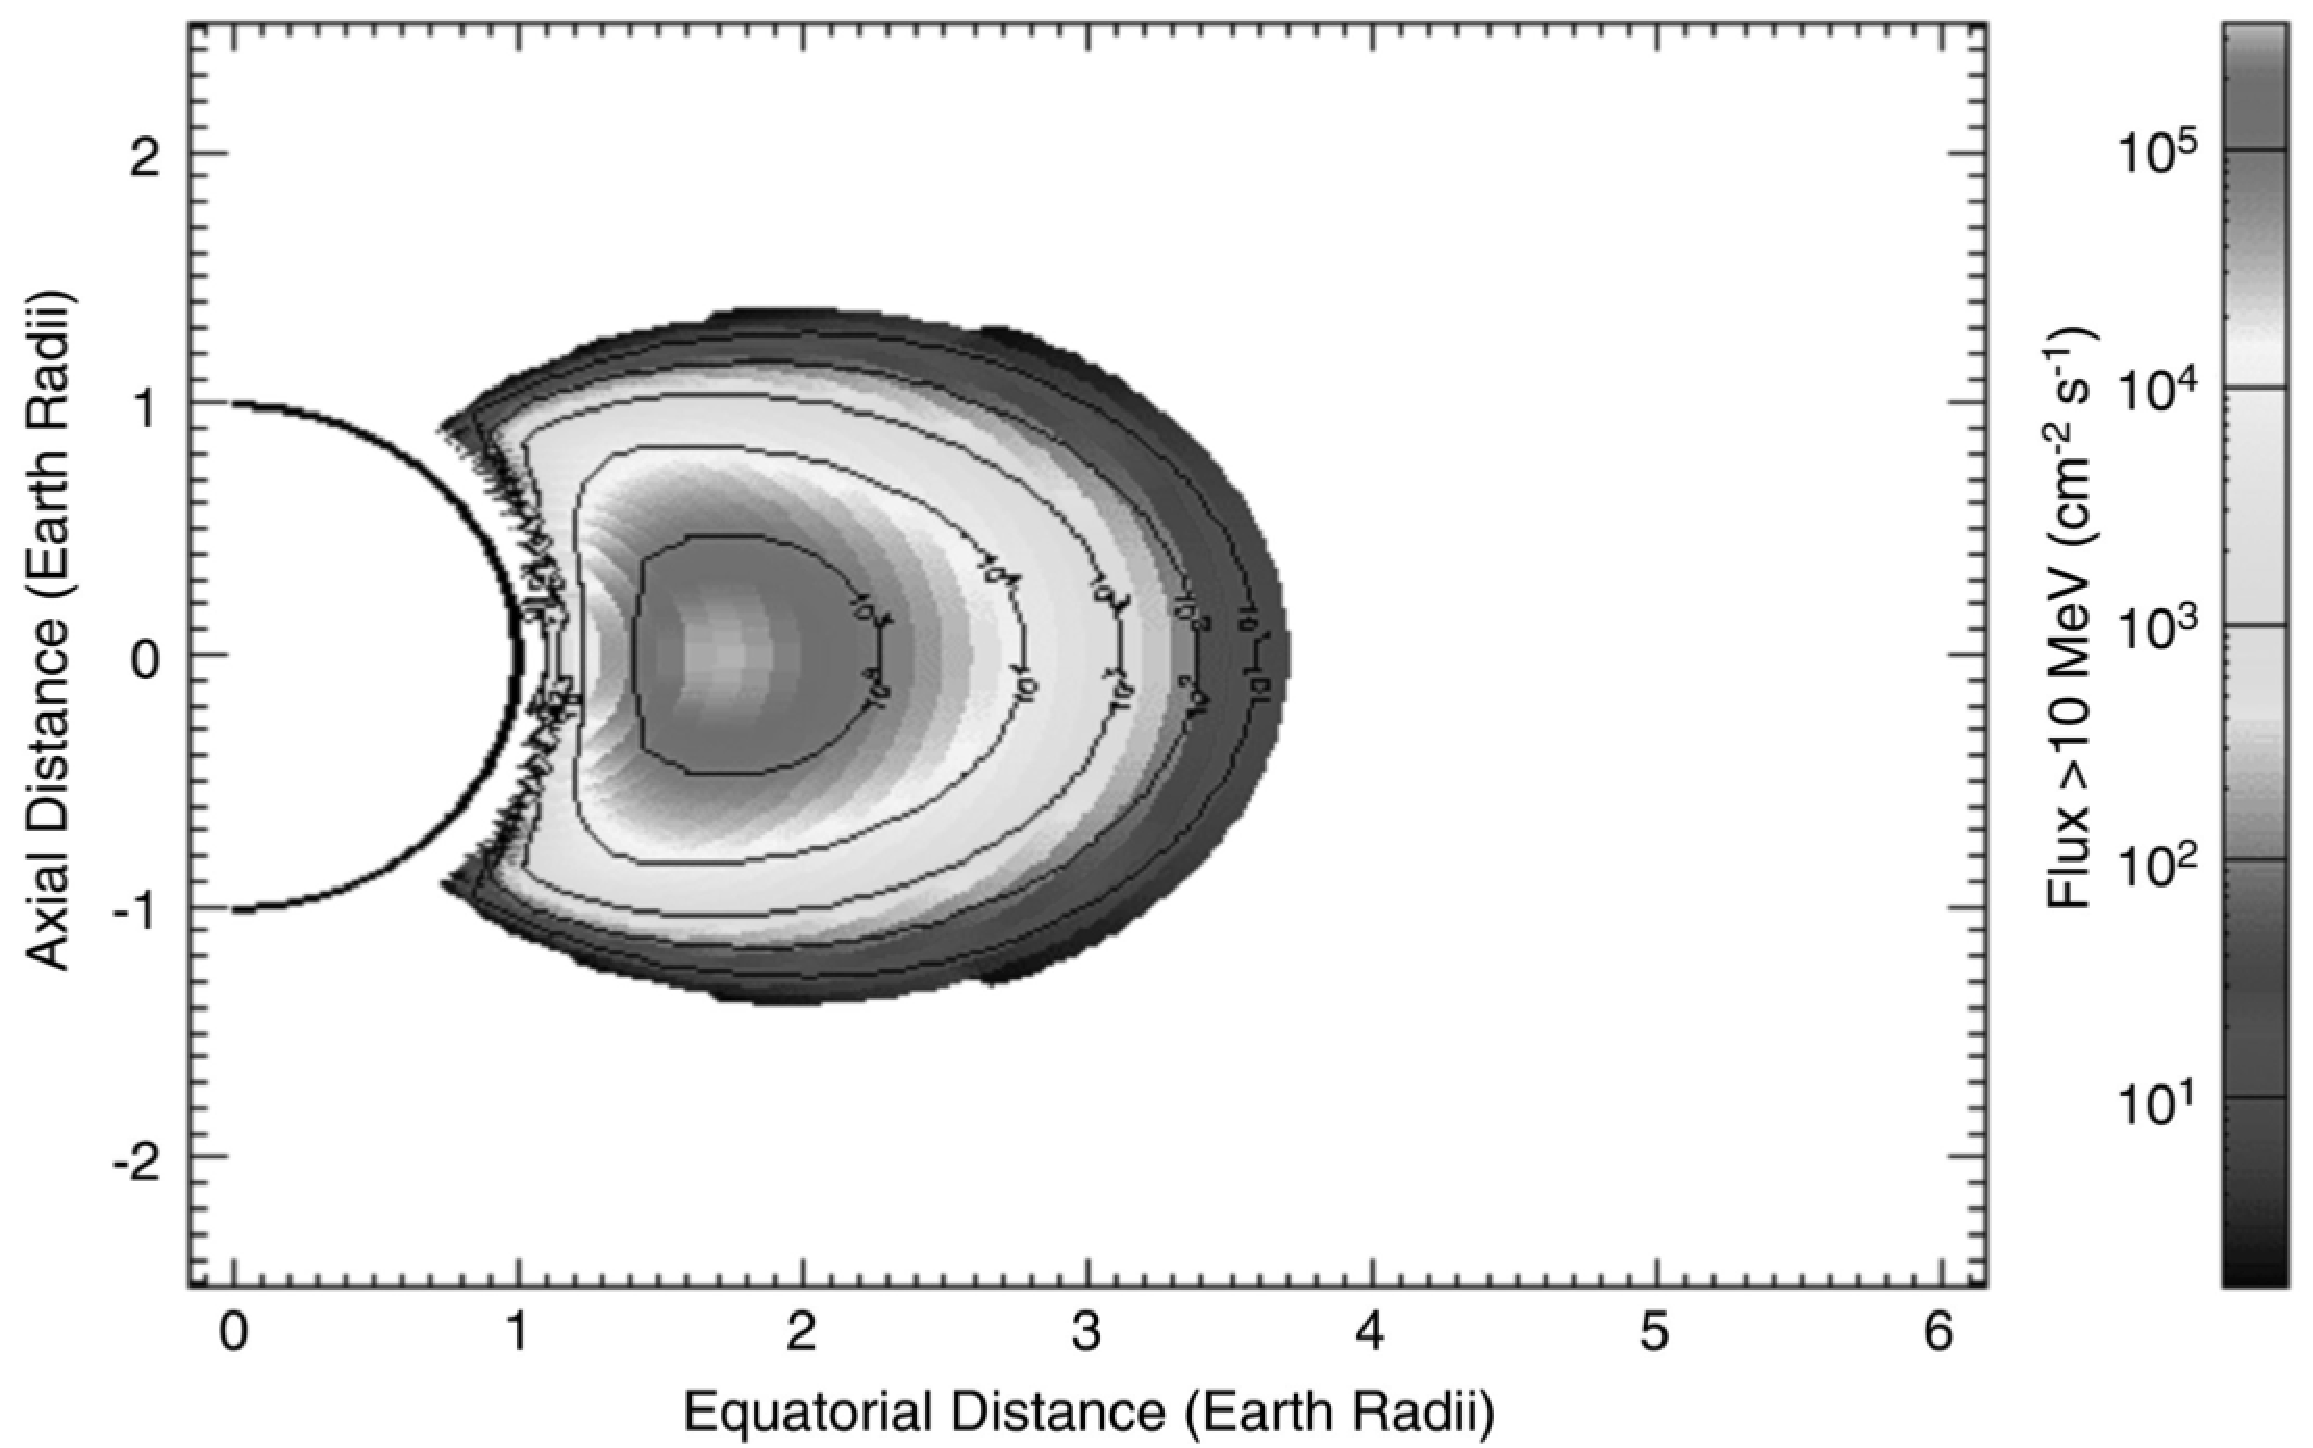
\includegraphics[width=5in]{xapsos_trapped_proton_env_earth.pdf}
    \end{center}
    \caption[The trapped proton population with energies $>$ 10 MeV as predicted by the AP-8 model for solar maximum conditions.]{The trapped proton population with energies $>$ 10 MeV as predicted by the AP-8 model for solar maximum conditions \cite{xapsos:2006}.}
    \label{fig:earth-trapped-protons}
\end{figure}
\begin{figure}[tb]
    \begin{center}
        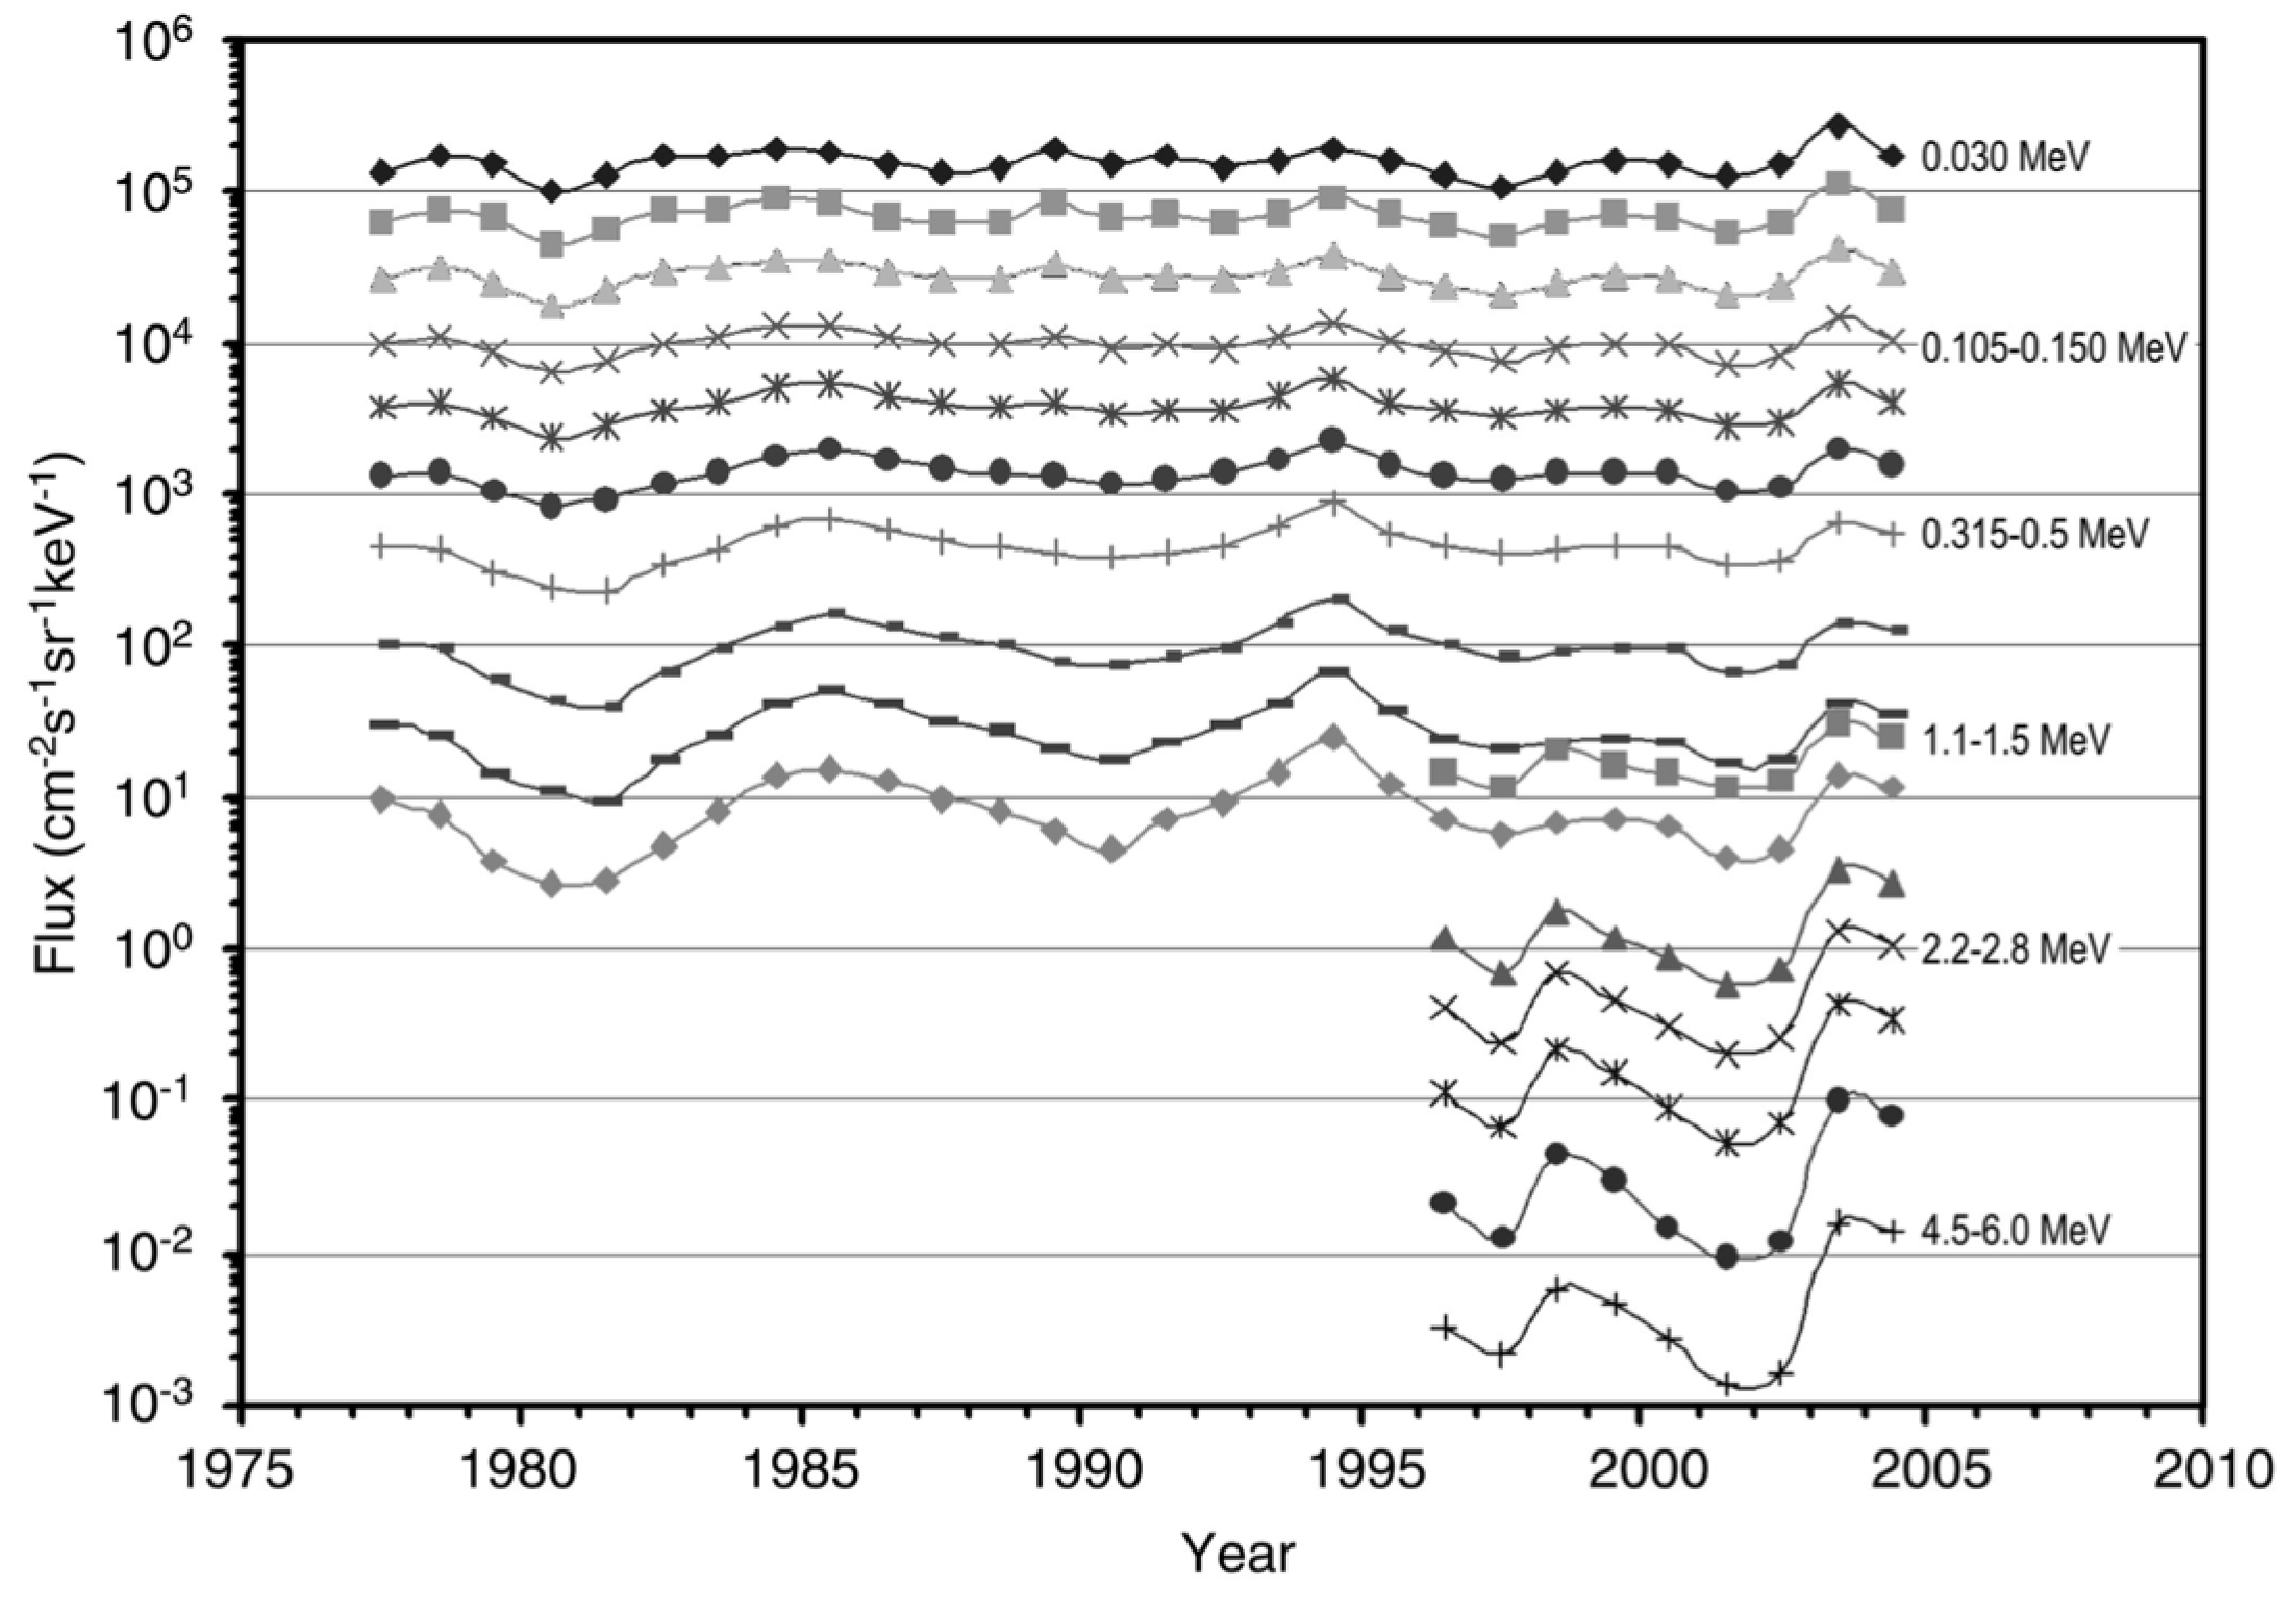
\includegraphics[width=5in]{xapsos_elec_geo_flux_vs_year_energy_curves.pdf}
    \end{center}
    \caption[Time and energy dependence of the mean electron flux at geostationary altitudes over about 2.5 solar cycles.]{Time and energy dependence of the mean electron flux at geostationary altitudes over about 2.5 solar cycles \cite{piet2006model}.}
    \label{fig:elec-geo-flux-vs-year}
\end{figure}


Trapped electrons around the Earth vary in energy from 10~keV to 10~MeV and are usually associated with TID, DD, and ESD/charging effects in electronic systems.
The differential flux of electrons as a function of time is shown in Fig.~\ref{fig:elec-geo-flux-vs-year}.
Fig.~\ref{fig:elec-geo-flux-vs-year} shows that for low-energy electrons ($<$1~MeV) electron flux at geostationary orbits have been relatively constant over time and do not vary significantly with solar activity.
This is not the case for high-energy($>$1~MeV) electrons, which vary as a function of time and solar activity.
Trapped electrons and protons exhibit regions of high flux in two distinct regions separated by the reduced flux slot region.
The inner radiation belts, for both electrons and protons, remain relatively stable and do not vary significantly with increased solar activity.
These inner regions contain the low to intermediate energy spectrum of electrons and protons.
This is not true for the slot regions, where variation in solar activity may  modulate the flux of particles by several orders of magnitude hour to hour and day to day.
The outer radiation belts exhibit a more significant dependence on solar activity varying in energy both flux by several orders of magnitude day to day.

Shielding has been used to great effect for electron environments near earth and in interplanetary space.
Only electrons with energy greater than 1~MeV are capable of transporting through 100~mils of aluminum and interacting with microelectronic systems.
In geostationary orbits, this amount of shielding provides fairly complete protection for electronic systems against TID and DD as very little of the trapped electron environment is capable of transporting through the shielding and impacting nominal system operation.
% subsubsection van_allen_radiation_belts (end)

\subsubsection{Jovian Electron Environment} % (fold)
\label{sub:jovian_environment}
Similar to that of Earth, Jupiter also exhibits a strong magnetic field surrounding the planet and has stable charged particle populations.
The energy associated with trapped electrons surrounding Jupiter is much greater than that of Earth \cite{divine1983charged,garrett2012galileo}.
The Jovian electron environment has been well studied by the galileo interim radiation electron (GIRE) model published by NASA-JPL \cite{divine1983charged}.
Additional efforts have extended the original GIRE model to a maximum energy of several hundred MeV and a maximum radius of 50 Jovian radii \cite{garrett2003galileo,garrett2005revised}.
The current version of the model, denoted as GIRE2, describes the omnidirectional flux of energetic electrons in the Jovian equatorial plane at distances large enough to extrapolate information for planned NASA missions to study the Jovian moons.

\begin{figure}[tb]
    \begin{center}
        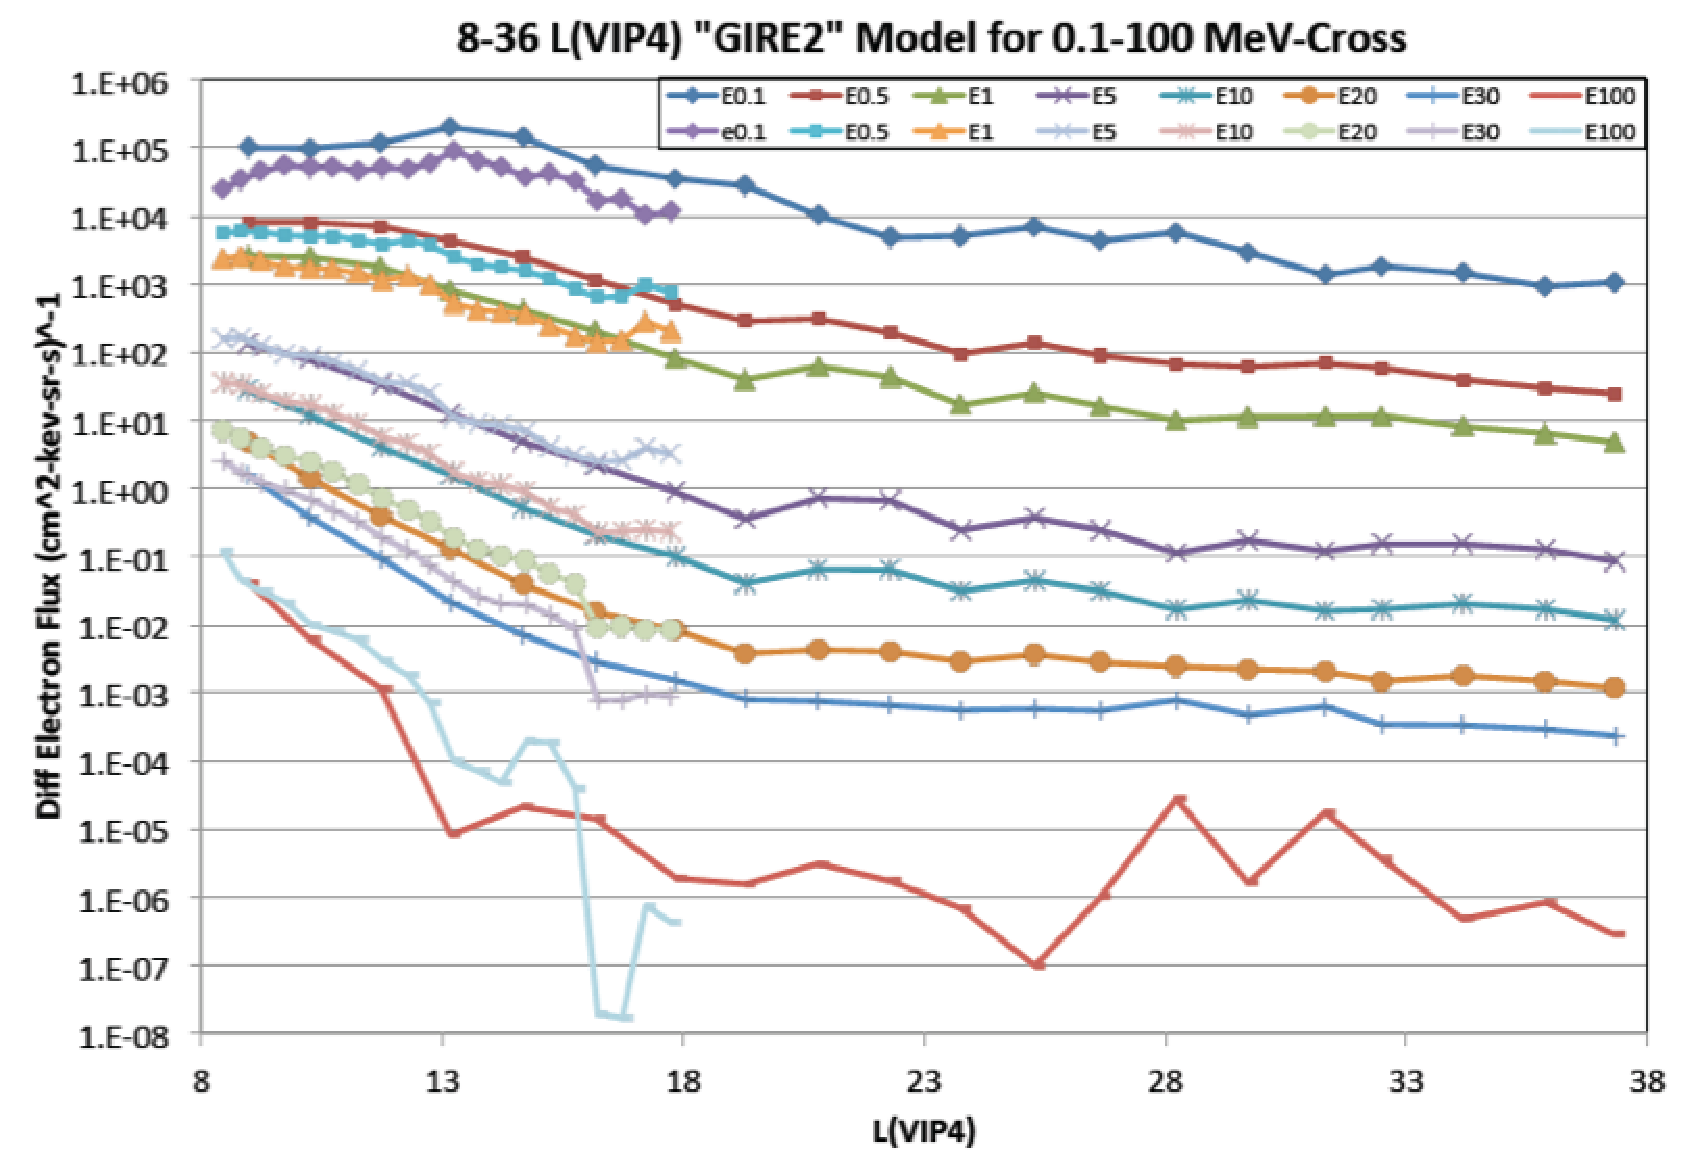
\includegraphics[width=5in]{gire2-line-plots-diffflux-jovianradii.pdf}
    \end{center}
    \caption[Line plots of the differential electron fluxes as predicted by the inner region GIRE and GIRE2 models.]{Line plots of the differential electron fluxes as predicted by the inner region GIRE and GIRE2 models \cite{garrett2012galileo}.}
    \label{fig:gire2-diff-flux}
\end{figure}
\begin{figure}[tb]
    \begin{center}
        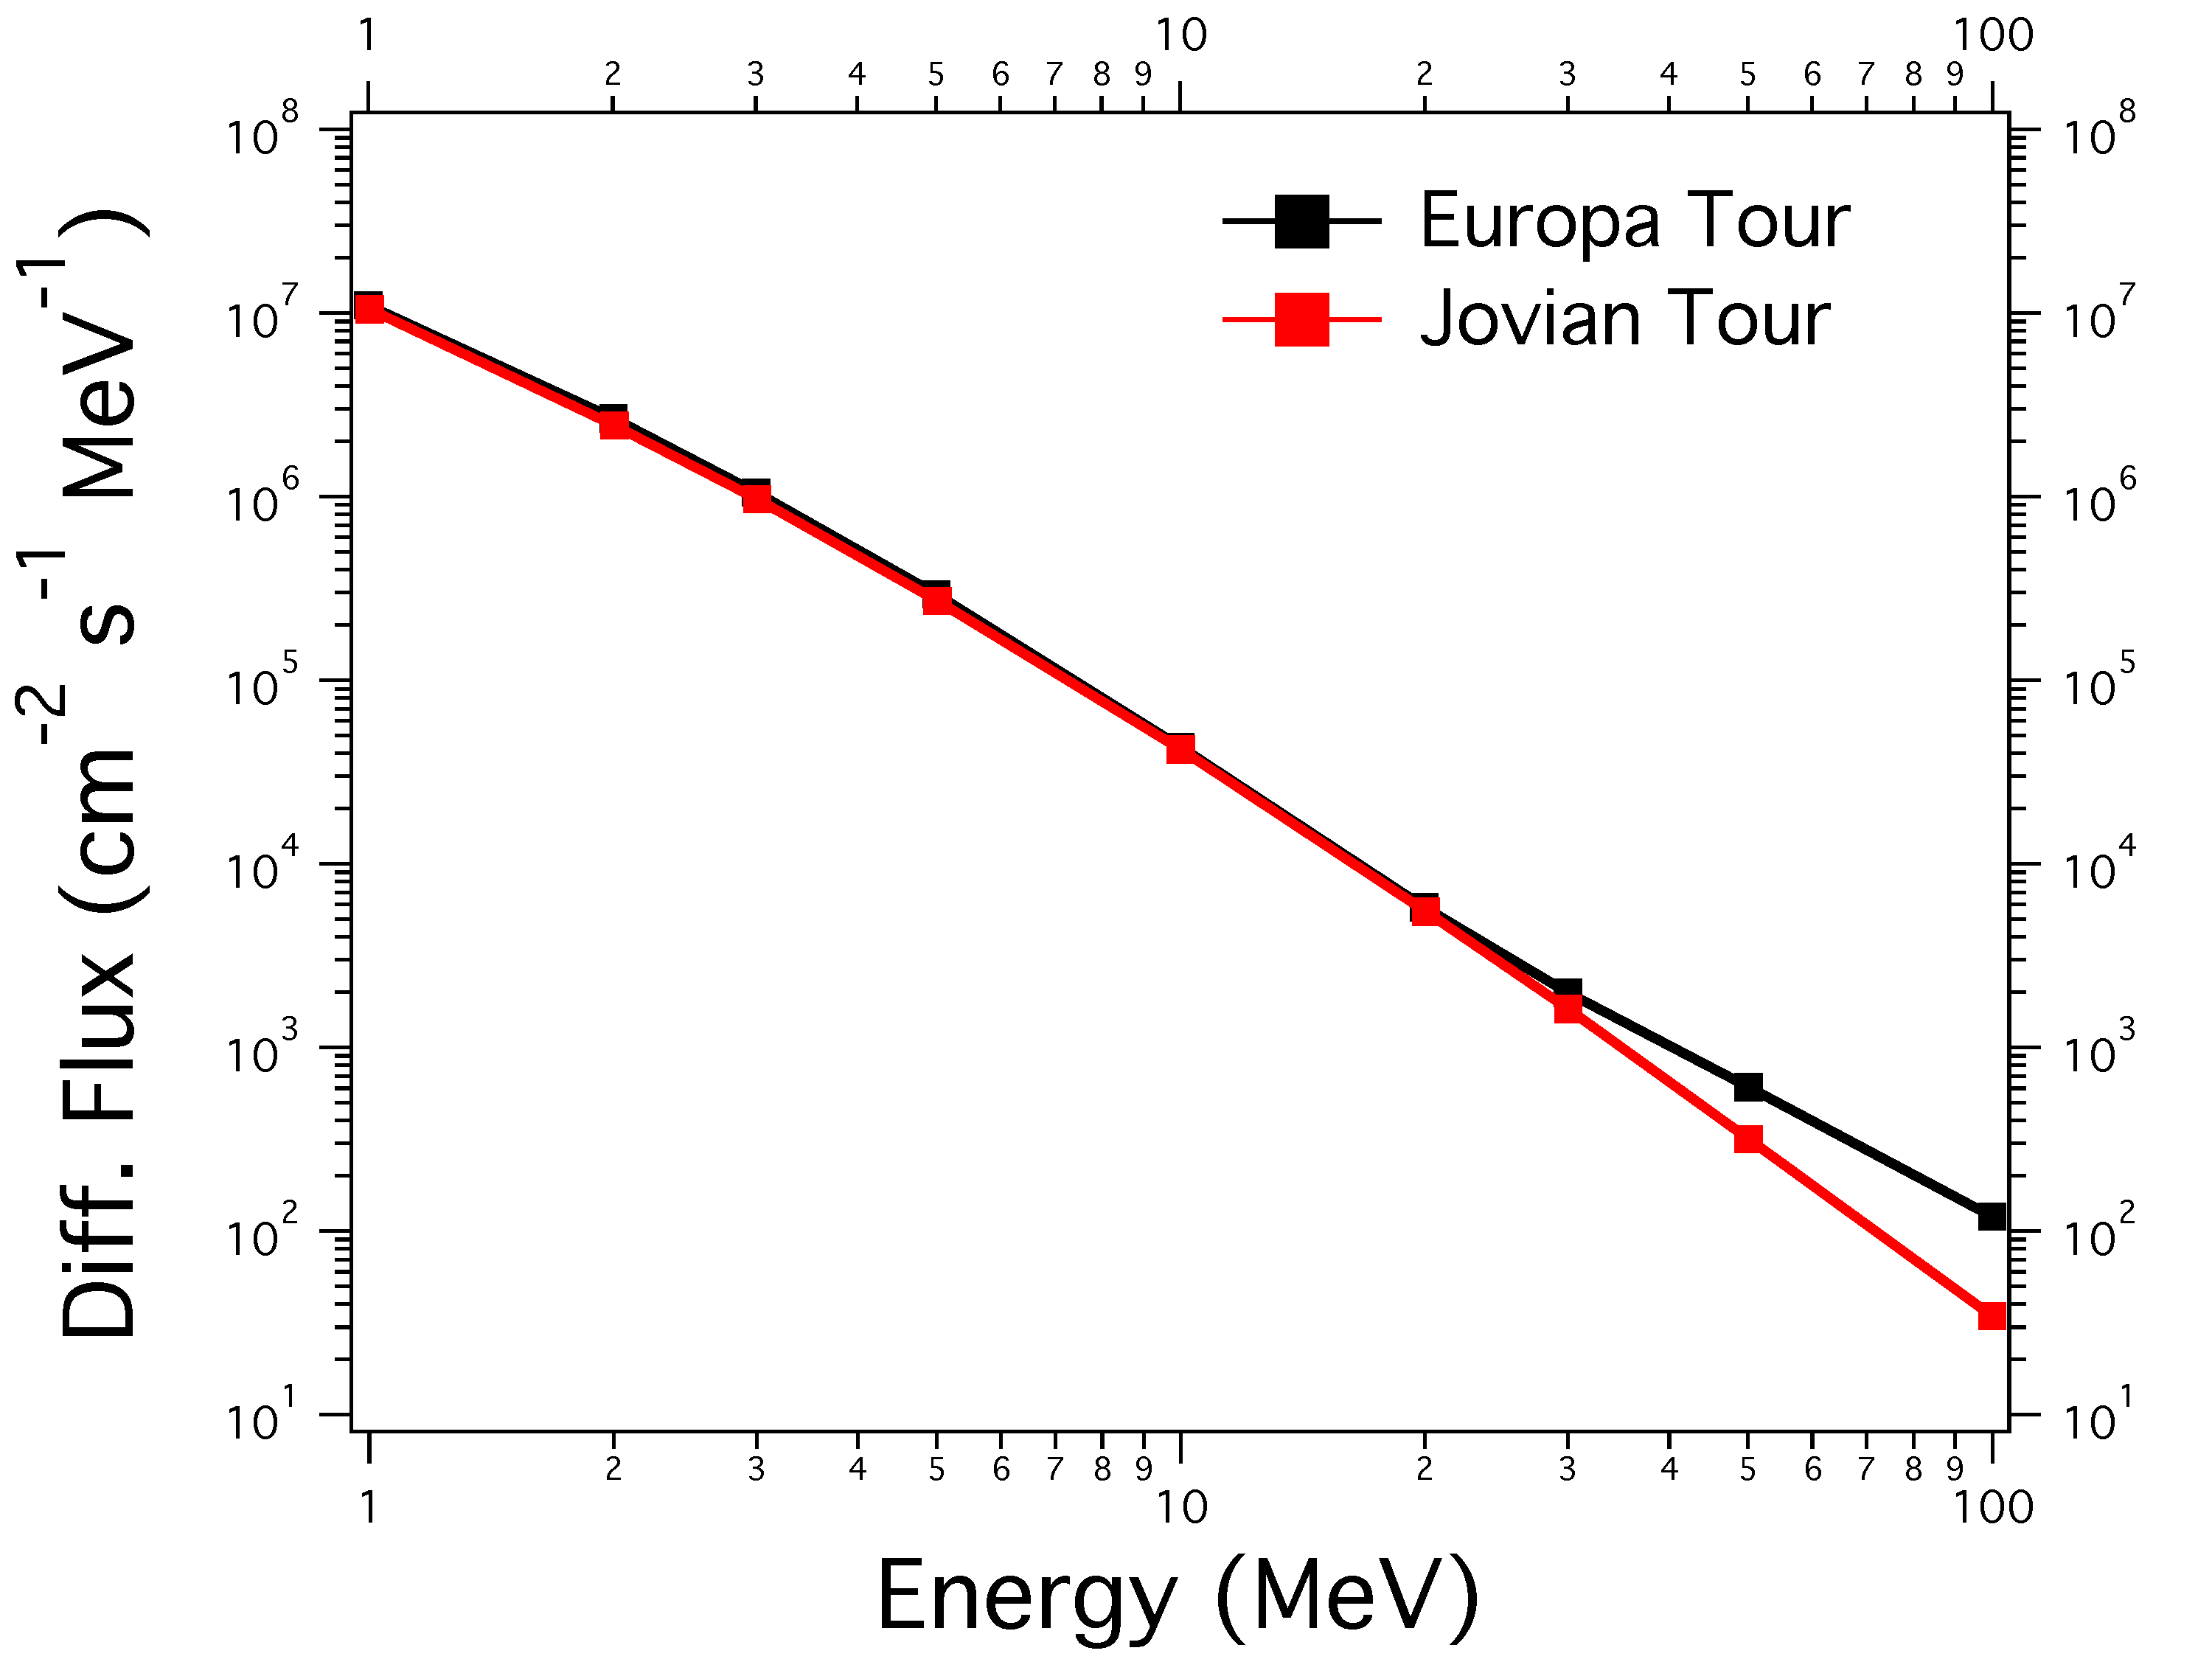
\includegraphics[width=5in]{nasa-jovian-missions-elec-env.pdf}
    \end{center}
    \caption{Differential flux spectrum for electrons in the Jovian and Europa environment phase of the Juno spacecraft mission to the Jupiter planetary system.}
    \label{fig:jovian-int-flux-spectrum}
\end{figure}

The differential flux spectrum as a function of distance, given in Jovian radii, is shown in Fig.~\ref{fig:gire2-diff-flux} with line plots indicating the flux of electrons of a given energy.
The energy spectrum of trapped electrons electrons in the Jovian environment ranges from approximately 10~keV to 100~MeV.
Similar to the trapped electron environment around Earth, there is significant variation in the estimated electron flux for high-energy ($>$10~MeV) with increasing distance.
Differences in the inner and outer radiation belts are due to distinct characteristics of the magnetic field surrounding Jupiter and are influenced heavily by fluctuations in solar activity \cite{garrett2012galileo}. 
Differential flux spectrum for electrons in the Jovian and Europa environment phase of the Juno spacecraft mission to the Jupiter planetary system can be seen in Fig.~\ref{fig:jovian-int-flux-spectrum}.
In the different phases of the Juno spacecraft tour of the Jupiter planetary system, onboard electronics will be exposed to a range of extremely energetic, high-flux electrons.
The 120~day tour of Europa alone results in a significant increase in the flux of electrons with energy higher than 20~MeV, which may have a significant impact on SEU event rates.
The use of 100~mils of aluminum shielding may provide protection for spacecraft electronic systems for the extremely high flux of electrons below 1~MeV. 
However, the flux of high-energy electrons is a non-negligible potentially serious threat for mission reliability. 
% subsubsection jovian_environment (end)

% subsection trapped_particle_environment (end)

% section radiation_environments (end)

\section{Ionizing Particle Track Structure} % (fold)
\label{sec:evaluating_track_structure}
Work by Kobetich \cite{Kobetich:1968im} and Katz \cite{Katz:1968fo} provided early understanding of ionization track structure in matter by modeling the range and stopping power of $\delta$-rays.
The Katz model represents the average energy deposited within a volume as a function of radial distance from an ion trajectory \cite{Chunxiang:1985uo, Fageeha:1994tc, Kobetich:1968im, Katz:1968fo}. 
Energy deposition occurs in regions surrounding an incident ion trajectory due to the scattering of $\delta$-rays, which results in spatially non-uniform, highly localized energy deposition events.

In \cite{Chunxiang:1985uo}, Zhang formulates an analytical expression of the dose deposited in the Katz model as a function of radial distance $t$,
\begin{equation}
    \label{eq:dose}
    D(t) = \frac{Ne^4Z^{*2}}{\alpha m_e c^2 \beta^2 t} \frac{(1-\frac{t-\theta}{T+\theta})^{1/\alpha}}{T+\theta}
\end{equation}
where $N$ is the electron density, $e$ is elementary charge, $m_e$ is the electron mass, $Z^*$ is the effective charge state of the incident particle with relative velocity $\beta$, $c$ is the speed of light in vacuum, $T$ is the range of $\delta$-rays with energy $W$, $\theta$ is the range of $\delta$-rays with kinetic energy equal to the ionization potential $I$, and $\alpha$ is a fitting parameter as defined in \cite{Chunxiang:1985uo, Fageeha:1994tc, Kobayashi:2004dg}.

\begin{figure}[htbp]
    \centering
        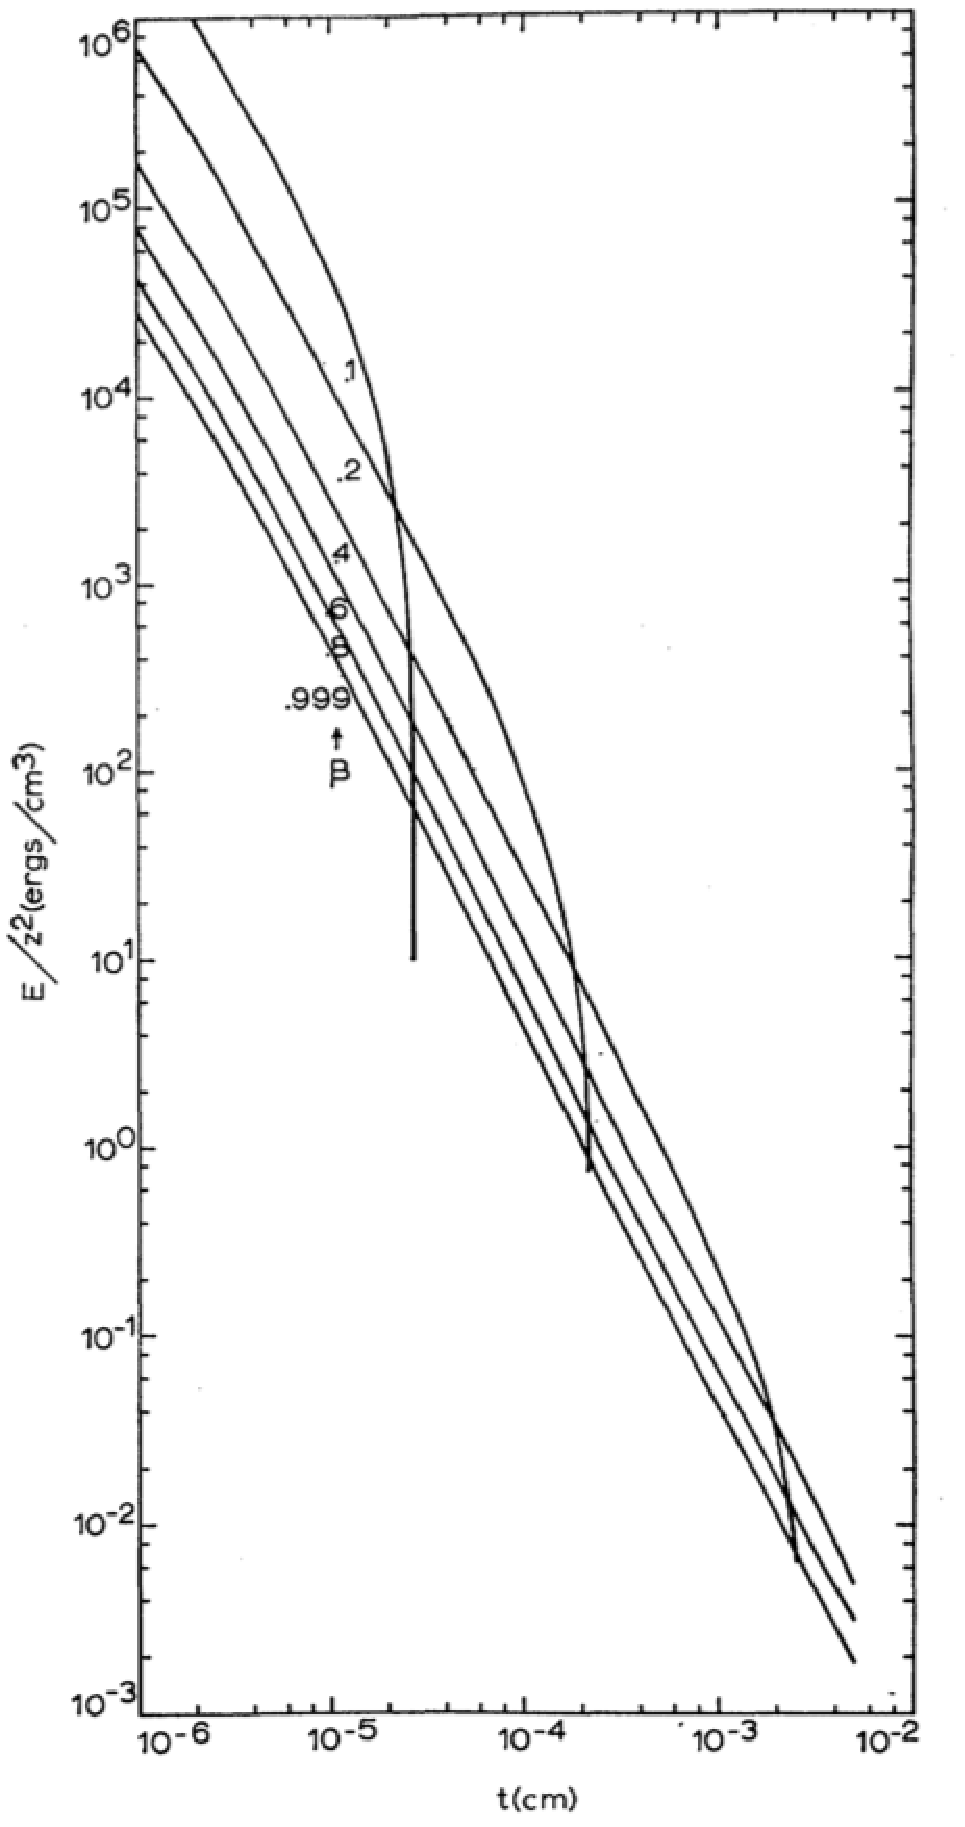
\includegraphics[height=7.5in]
        {katz_dose_in_emulsion.pdf}
    \caption[The spatial distribution of ionization energy in water for incident particles with differing relative velocity. These calculations, based on Katz theory, describe the average dose deposited as a function of radial distance, $t$, from the incident ion track.]{The spatial distribution of ionization energy in water for incident particles with differing relative velocity \cite{Kobetich:1968im,Katz:1968fo,Katz:1969uo}. These calculations, based on Katz theory, describe the average dose deposited as a function of radial distance, $t$, from the incident ion track.}
    \label{fig:katz_dose_in_water}
\end{figure}

Fig.~\ref{fig:katz_dose_in_water} shows the radial dose profile in emulsion for several incident ion energies \cite{Kobetich:1968im,Katz:1968fo,Katz:1969uo}. 
The radial extension of the ionization track structure depends on the energy of the incident ion due to the kinematics of $\delta$-ray generation and their range.
For small values of incident ion energy, Fig.~\ref{fig:katz_dose_in_water} shows the radial dose deposited is larger near the core of the ion track. 
As $\beta$ increases, Fig.~\ref{fig:katz_dose_in_water} shows that the dose near the ion track core decreases, while the corresponding maximum radial distance energy is deposited increases.

The kinematics of $\delta$-ray generation limit the maximum energy transferable in a collision between an incident ion and a single electron. 
This limitation on energy transfer restricts a $\delta$-ray's transport range within the target material. 
The expression for maximum energy transfer, $W$, is given by
\begin{equation}
    \label{eq:emax}
    W = 2m_{e}c^2\gamma^2\beta^2
\end{equation}
where $m_e$ is the rest mass of an electron, $c$ is the speed of light, $\beta$ is the relative velocity of the incident ion, and $\gamma$ is the Lorentz factor (defined as $(1-\beta^2)^{-1/2}$).
Equation~(\ref{eq:emax}) is valid for the case $\gamma m_e / M_{ion} \ll 1$, where $M_{ion}$ is the mass of the incident ion. 
Equation~(\ref{eq:emax}) scales monotonically with incident ion energy; this implies that for very energetic particles, generated $\delta$-rays may transport far from their point of generation.
As the incident ion loses energy, the track radius decreases, forming a conical shape as a function of distance into the target material \cite{Stapor:1988ws}.

In 1988, Stapor \emph{et al.} described how two particles with similar LETs would have vastly differing charge generation profiles, and therefore the possibility for differing SEU responses \cite{Stapor:1988ws}.
In Fig.~\ref{fig:1988_stapor_cu_ions}, \emph{e-h} pair density is plotted as a function of radial distance from the ion trajectory at a depth of 1~$\mu$m in silicon.
Fig.~\ref{fig:1988_stapor_cu_ions} illustrates the difference in the resulting charge generation profiles for two ions with similar LETs but differing energies \cite{Stapor:1988ws}. 
\begin{figure}[htbp]
    \centering
        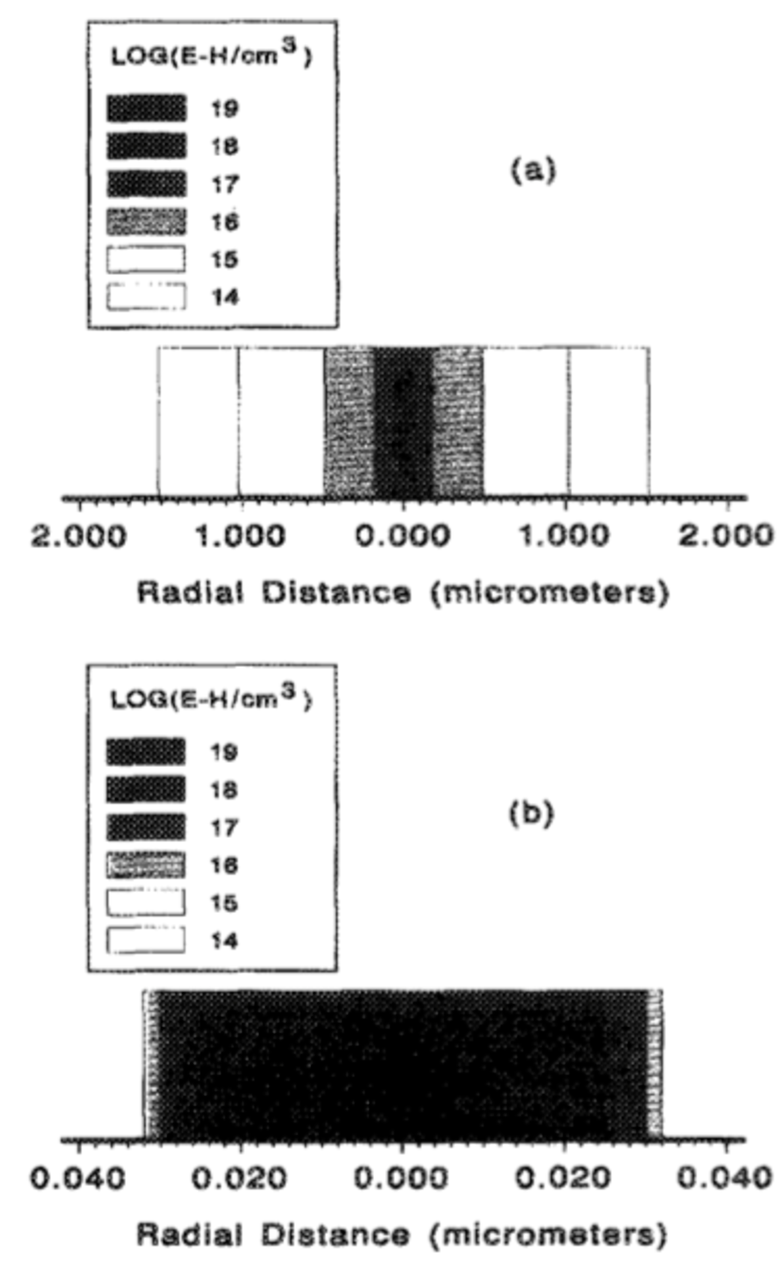
\includegraphics[width=4in]
        {stapor_1988_let_26_Cu_ions.pdf}
    \caption[Calculated \emph{e-h} pair density generation is shown as a function of radial distance from the ion track at a depth of 1 $\mu$m within a volume of silicon for (a) 395 MeV Cu and (b) 25 MeV Cu.]{Calculated \emph{e-h} pair density generation is shown as a function of radial distance from the ion track at a depth of 1 $\mu$m within a volume of silicon for (a) 395 MeV Cu and (b) 25 MeV Cu \cite{Stapor:1988ws}.}
    \label{fig:1988_stapor_cu_ions}
\end{figure}
While the LET of a 25~MeV and 395~MeV Cu ion is the same, the resulting charge generation profiles differ, with the less energetic particle having a very dense charge generation region around the core of the ion trajectory, and the more energetic ion having a greater radial extension from the incident ion trajectory.
As the incident particle loses energy, the maximum energy of generated $\delta$-rays also decreases, causing the ion track radius to decrease with increasing penetration depth into the material.

In 1992, Xapsos \cite{Xapsos:1992tc} outlined a statistical framework for the application of LET to microelectronics that considered the track structure of an incident ion. 
This firmly established a metric for determining the validity of LET for technology nodes with well-established sensitive volume geometries. 
Dodd \emph{et al.} \cite{Dodd:1998tn} published measurements six years later showing the LET metric was sufficient to characterize CMOS technology nodes larger than 250 nm.
In \cite{Dodd:1998tn}, Dodd effectively demonstrates that for older technology nodes that exhibit a critical charge greater than 10~fC the LET of the primary particle is sufficient to predict the device- and circuit-level response.

More recently, interest has reemerged in evaluating the potential contribution of electrons and $\delta$-rays to the SEU response of modern technology nodes.
Murat \emph{et al.} evaluated technology nodes with feature sizes less than 0.5~$\mu$m, determining that the energy of the incident ion does contribute to the SEU response \cite{Murat:kk}.
Later, King \emph{et al.} demonstrated the potential for contributions to the SEU cross section from individual $\delta$-rays depositing energy within the sensitive volume of a 22~nm SRAM \cite{King:2010cu}.
Raine \emph{et al.} published several papers utilizing the Katz model to evaluate energy deposition contributions from $\delta$-rays in a single ionizing particle event to the SEU rate. 
These studies concluded that the ionization profile of heavy ions does not contribute to multiple-bit upsets in the 32~nm SOI technology node \cite{Raine:gk}.
However, it has been shown that while the average energy deposition profile is modeled very well by the Katz model, variation between the average and individual $\delta$-ray energy deposition events can be quite significant \cite{King:2012cb}.

\begin{figure}[htbp]
    \centering
    \subfigure[]
    {
    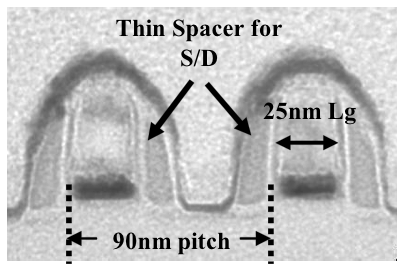
\includegraphics[width=2.5in]{haran-transistors.png}
    \label{fig:2008_22nm_trans_haran}
    }
    \subfigure[]
    {
    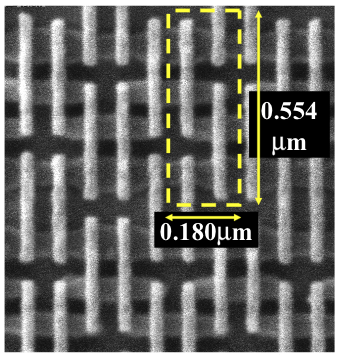
\includegraphics[width=2.5in]{haran-sram.png}
    \label{fig:2008_22nm_sram_haran}
    }
    \caption[\ref{fig:2008_22nm_trans_haran}~Cross-sectional TEM image showing thin composite oxide-nitride spacer on 25~nm wide gate at 90~nm pitch. \ref{fig:2008_22nm_sram_haran}~Top-down SEM image of the 0.1~$\mu$m$^2$ 6T-SRAM cell after STI fill and gate-first metal gate patterning, with cell dimensions of 0.18~$\mu$m and 0.554~$\mu$m.]{\ref{fig:2008_22nm_trans_haran}~Cross-sectional TEM image showing thin composite oxide-nitride spacer on 25~nm wide gate at 90~nm pitch. \ref{fig:2008_22nm_sram_haran}~Top-down SEM image of the 0.1~$\mu$m$^2$ 6T-SRAM cell after STI fill and gate-first metal gate patterning, with cell dimensions of 0.18~$\mu$m and 0.554~$\mu$m. After \cite{Haran:2008ta}.}
    \label{fig:ibm_22nm_trans_sram_spacing}
\end{figure}

The track radius of ionizing radiation events is large compared to the spacing of adjacent transistors and pitch of neighboring SRAM cells in a 22~nm technology node, shown in Fig.~\ref{fig:ibm_22nm_trans_sram_spacing}.
This implies that modern technology nodes have scaled to a point where electron/$\delta$-ray energy deposition events may be of sufficient magnitude and interact frequently enough to become a reliability concern.
This leads to the potential for contributions to the single- and multiple-bit upset event rate from the primary ion and $\delta$-rays generated in ionizing particle events.
Consequently, for technologies that exhibit critical charges lower than 0.2~fC, the role of $\delta$-rays must be reconsidered when evaluating the SEU response of SRAM fabricated in these technology nodes \cite{King:2010cu, King:2012cb}.
It is therefore necessary to have a thorough understanding of the potential implications of $\delta$-rays on these devices in order to understand the SEU response of SRAMs fabricated in that technology nodes that exhibit small critical charge.
These issues are discussed in detail in Chapter~\ref{sec:impact_of_delta_rays_on_microelectronics}, which focuses on the impact of incident ion species, energy, mass, and the implications of $\delta$-rays interactions on the SEU response of current- and next-generation technology nodes.
% section sec:evaluating_track_structure (end)

% chapter background (end)
